\newpage
\section{Inspection images}\label{ap:inspec_img}
 % \todo[inline]{Optical microscope images of mask}
\begin{figure*}[htb]
    \centering
    \begin{subfigure}[t]{0.24\linewidth}
        \resizebox{\linewidth}{!}{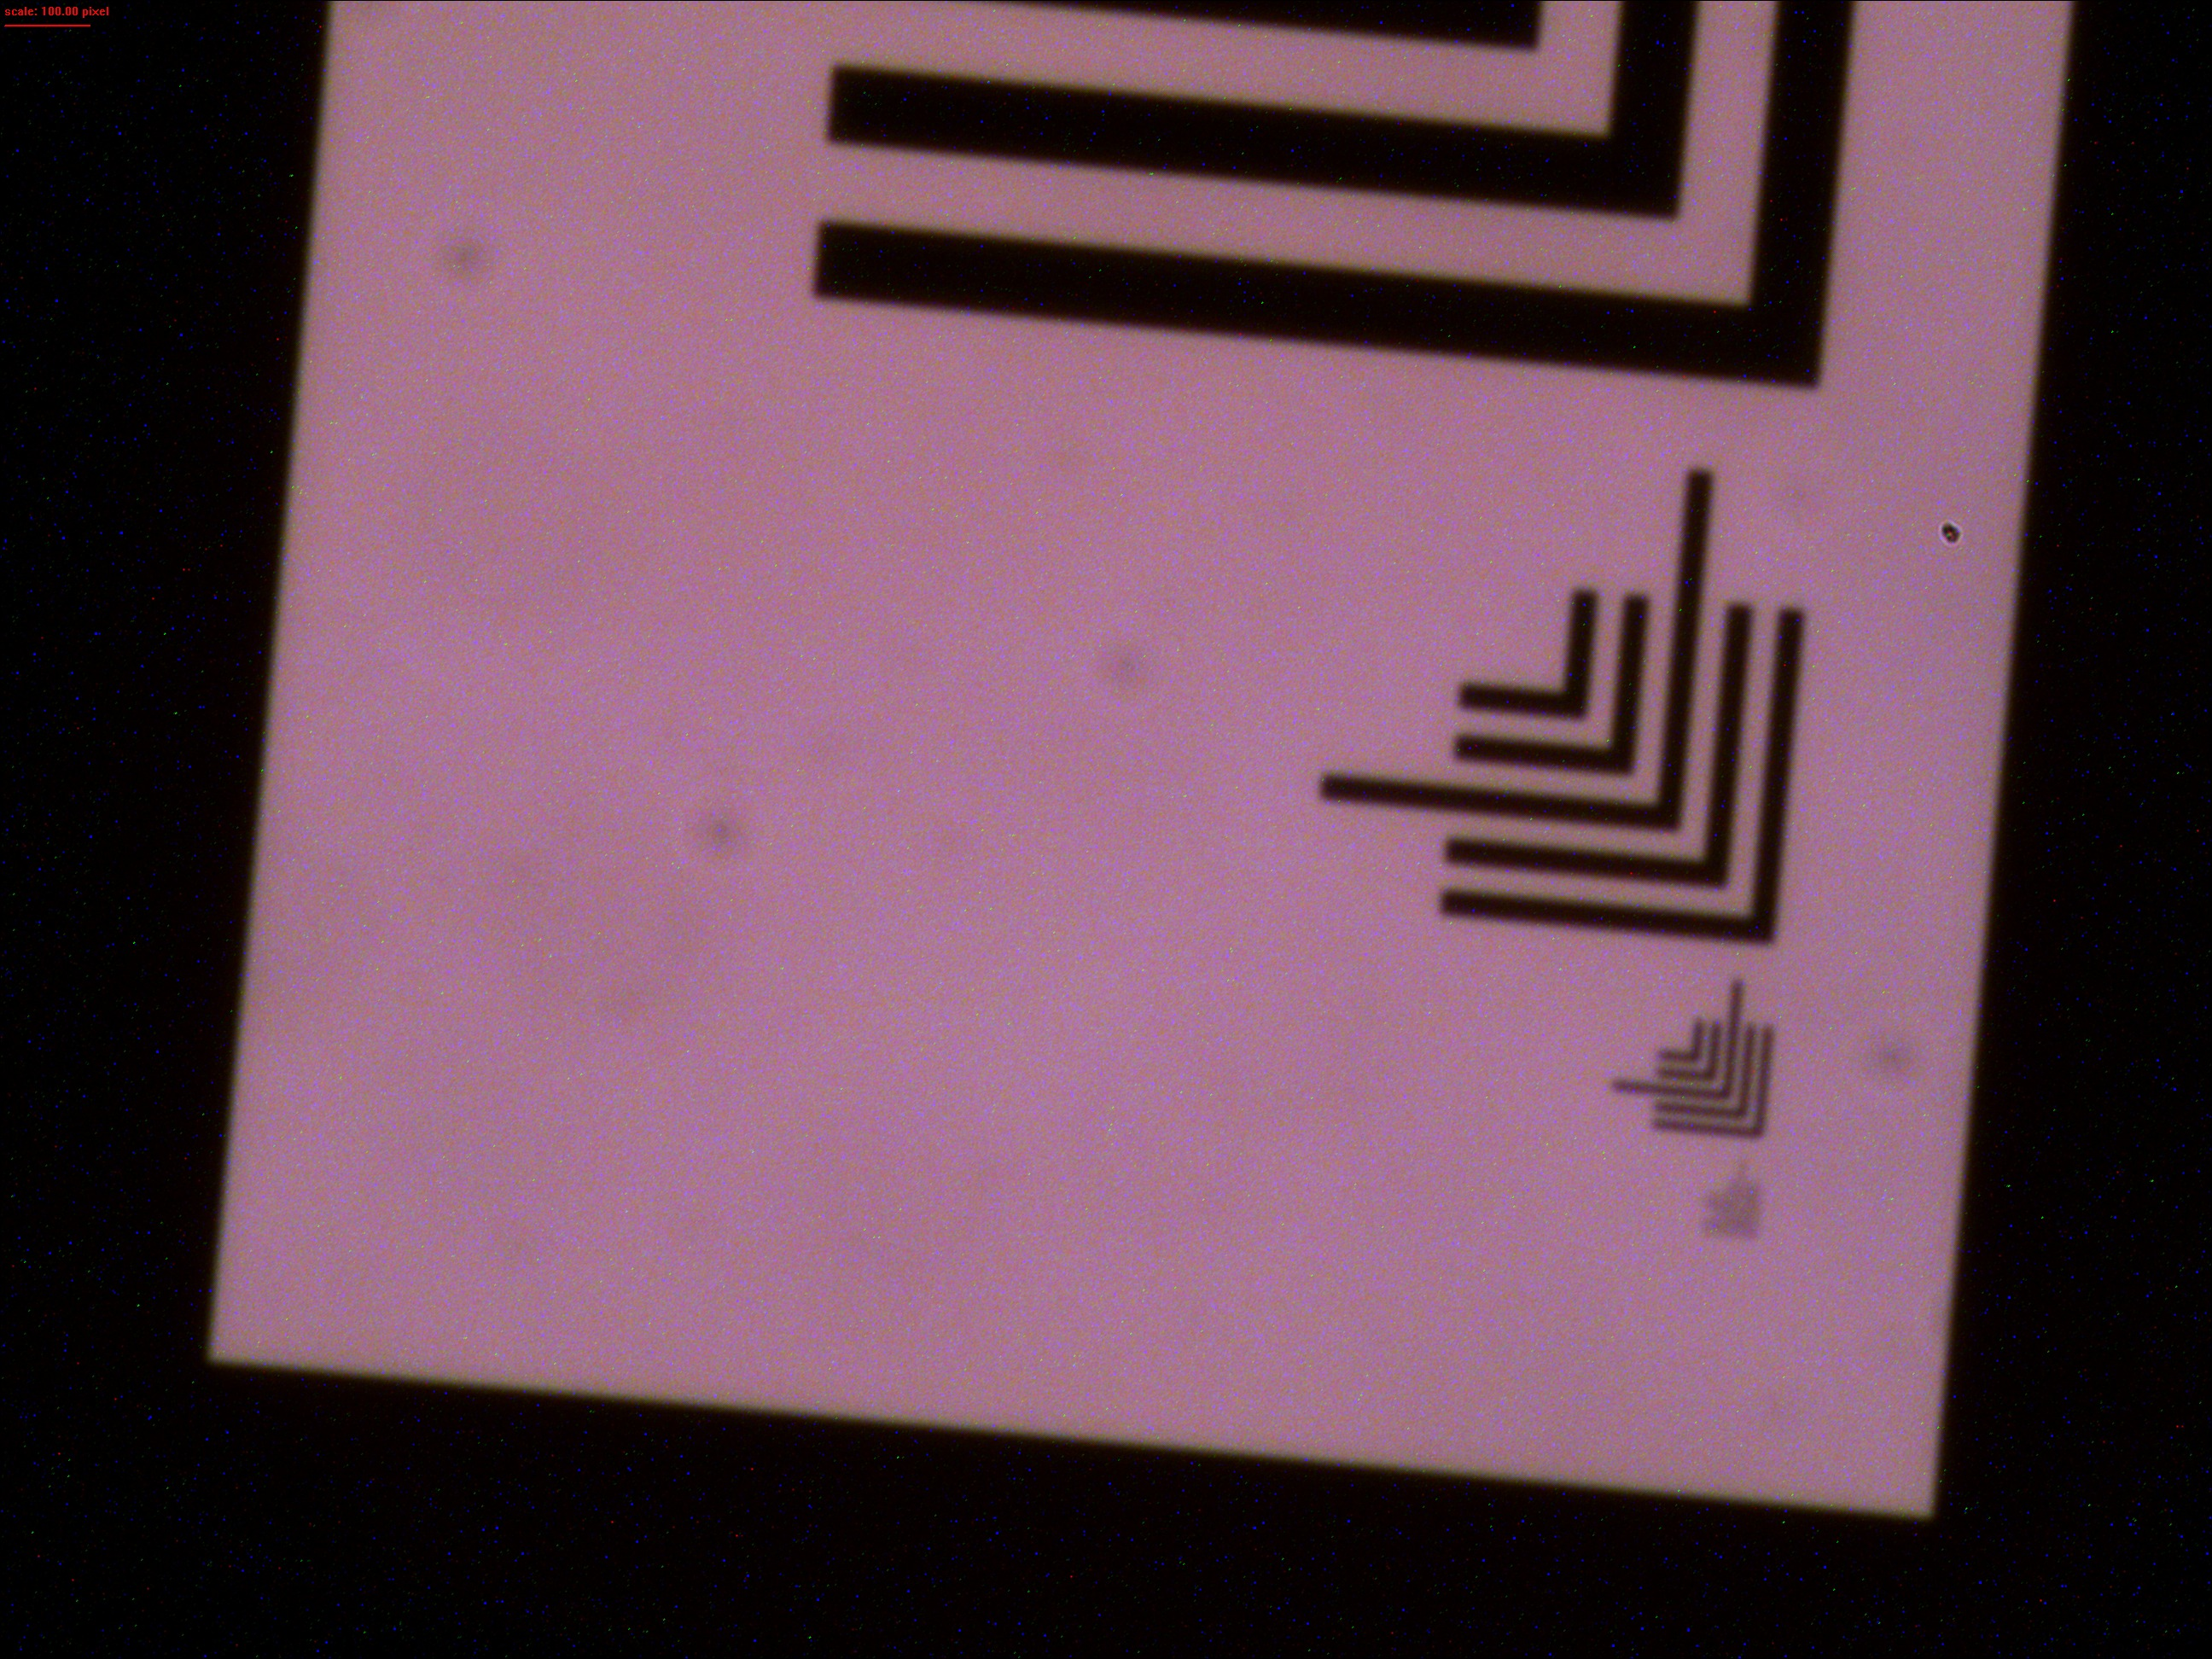
\includegraphics{data/mask/TS_05_20_13_50_44.jpg}}
      	\caption{Single line surrounded by multiple lines pattern at several length scales.}
      	\label{fig:TS_05_20_13_50_44}
    \end{subfigure}
    \hfill
    \begin{subfigure}[t]{0.24\linewidth}
      	\resizebox{\linewidth}{!}{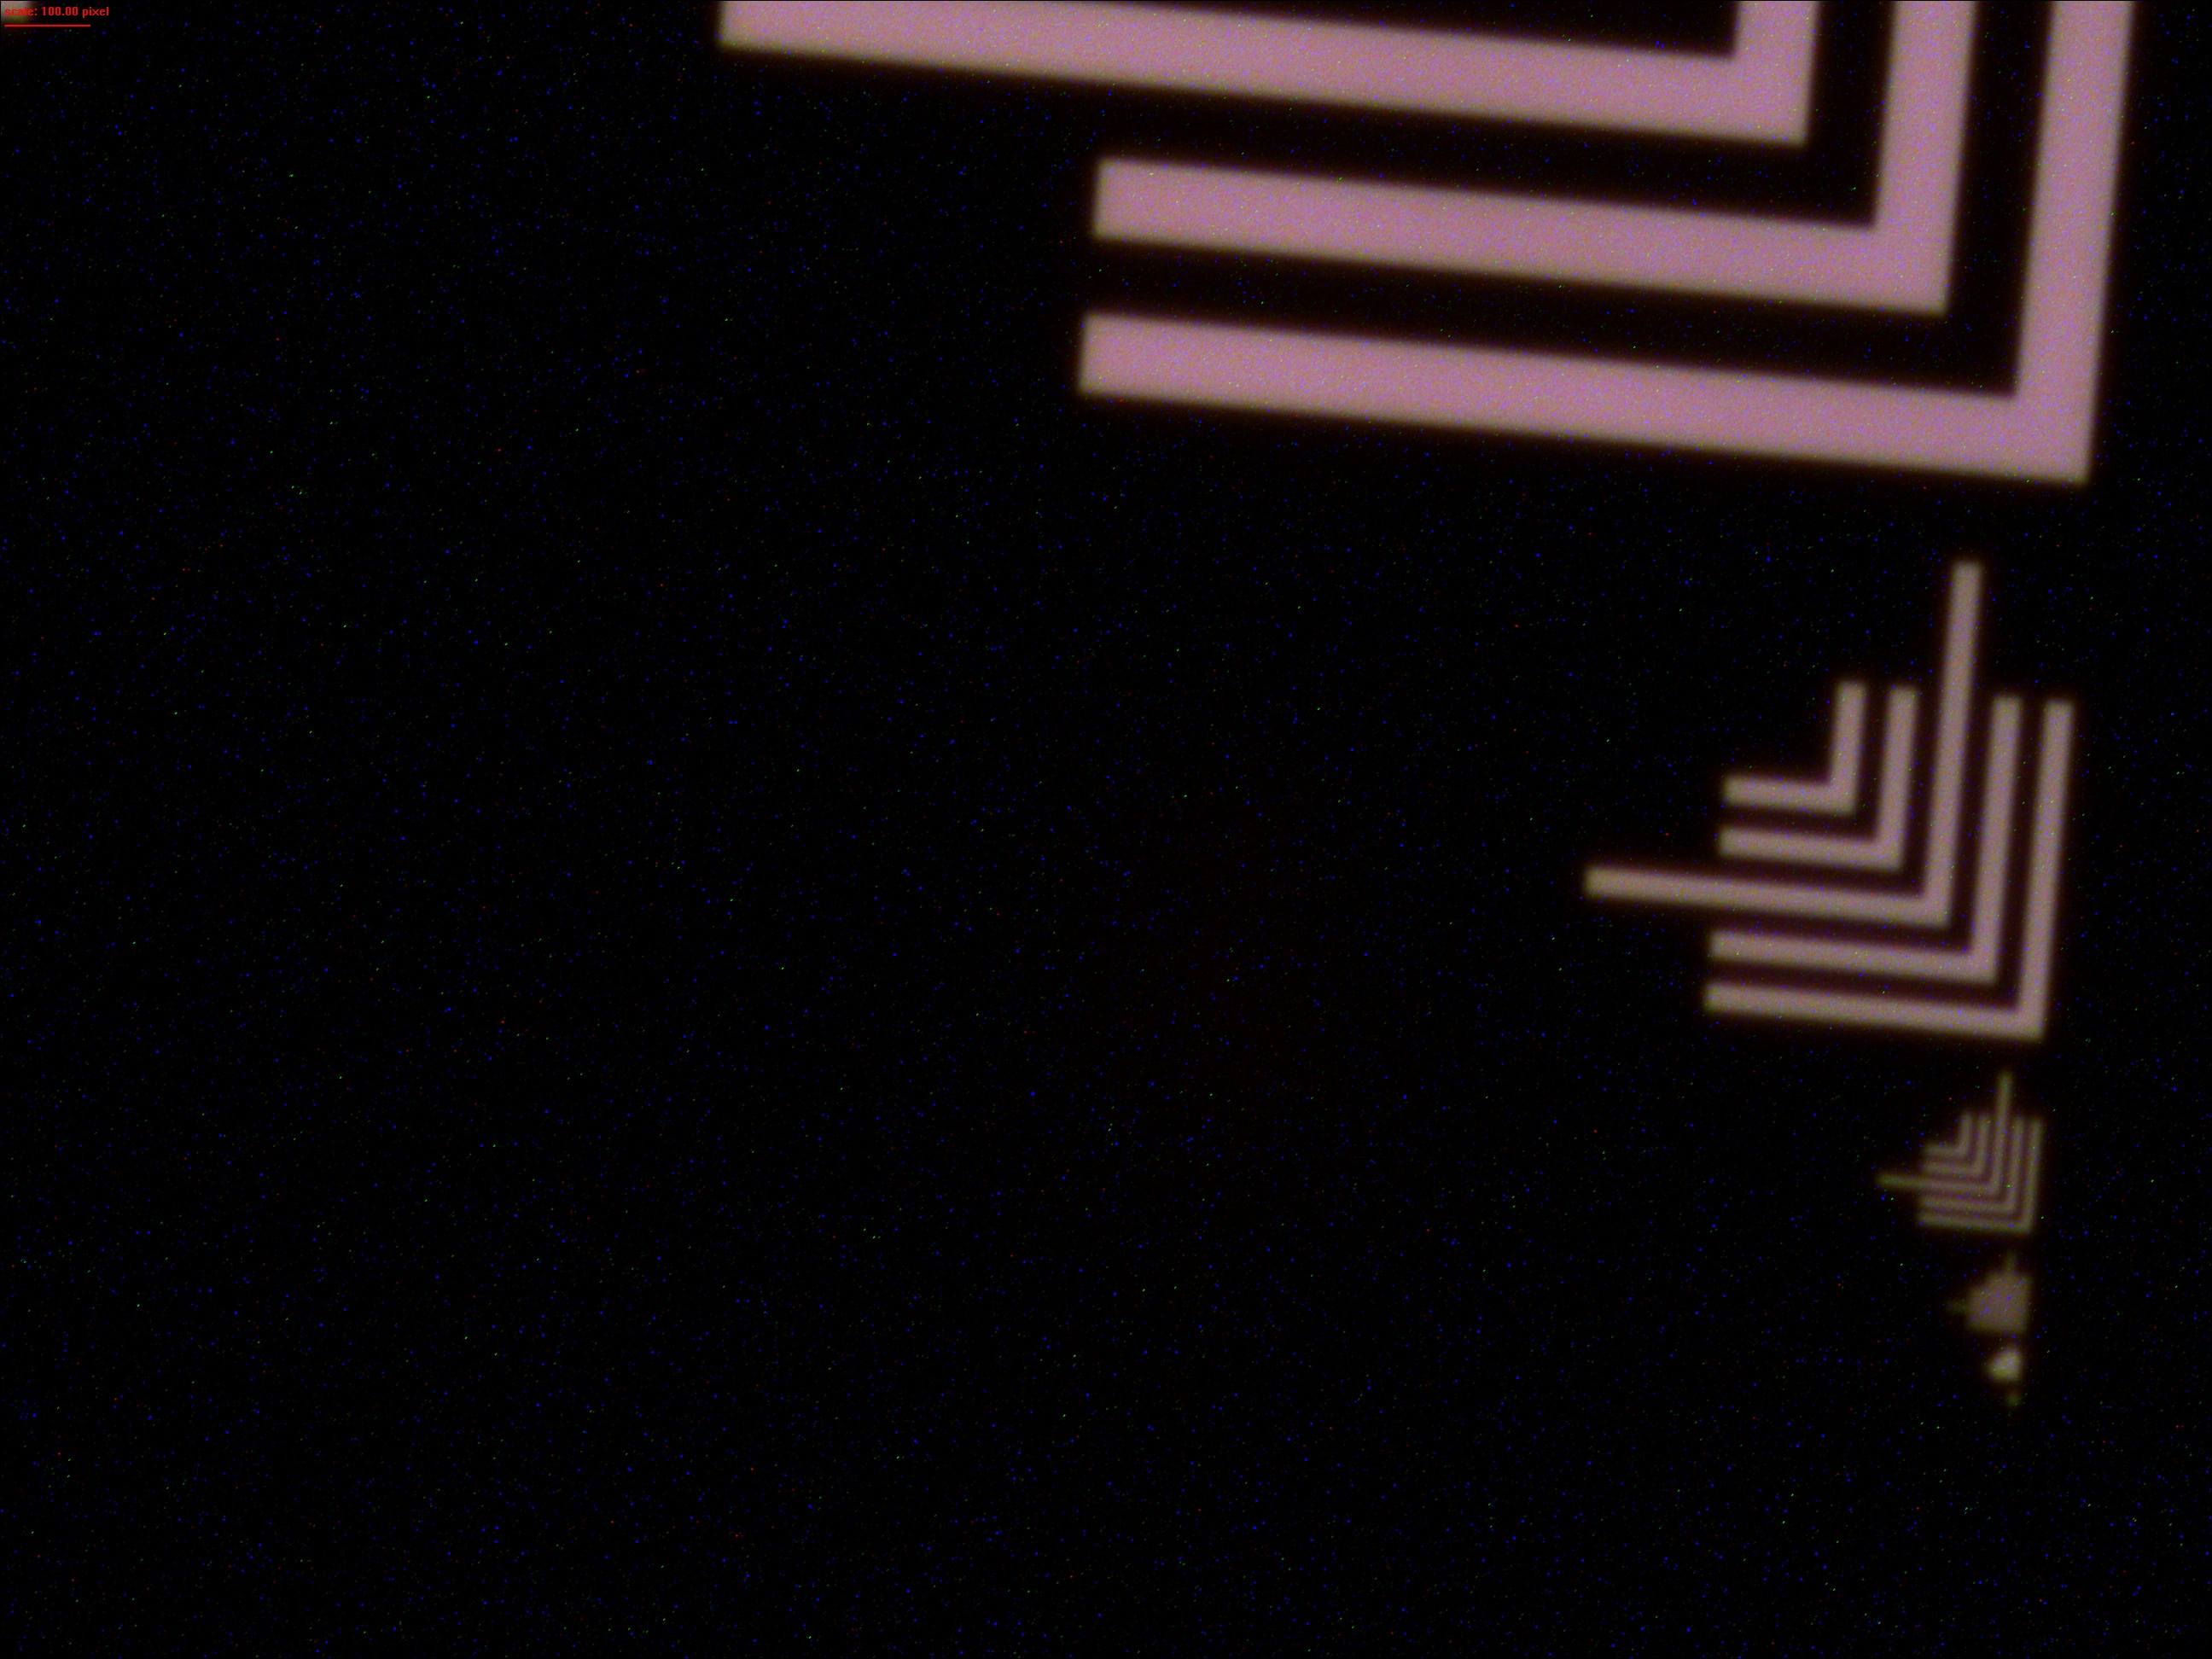
\includegraphics{data/mask/TS_05_20_13_51_16.jpg}}
      	\caption{Inverse of the previous pattern.}
      	\label{fig:TS_05_20_13_51_16}
    \end{subfigure}
    \hfill
    \begin{subfigure}[t]{0.24\linewidth}
      	\resizebox{\linewidth}{!}{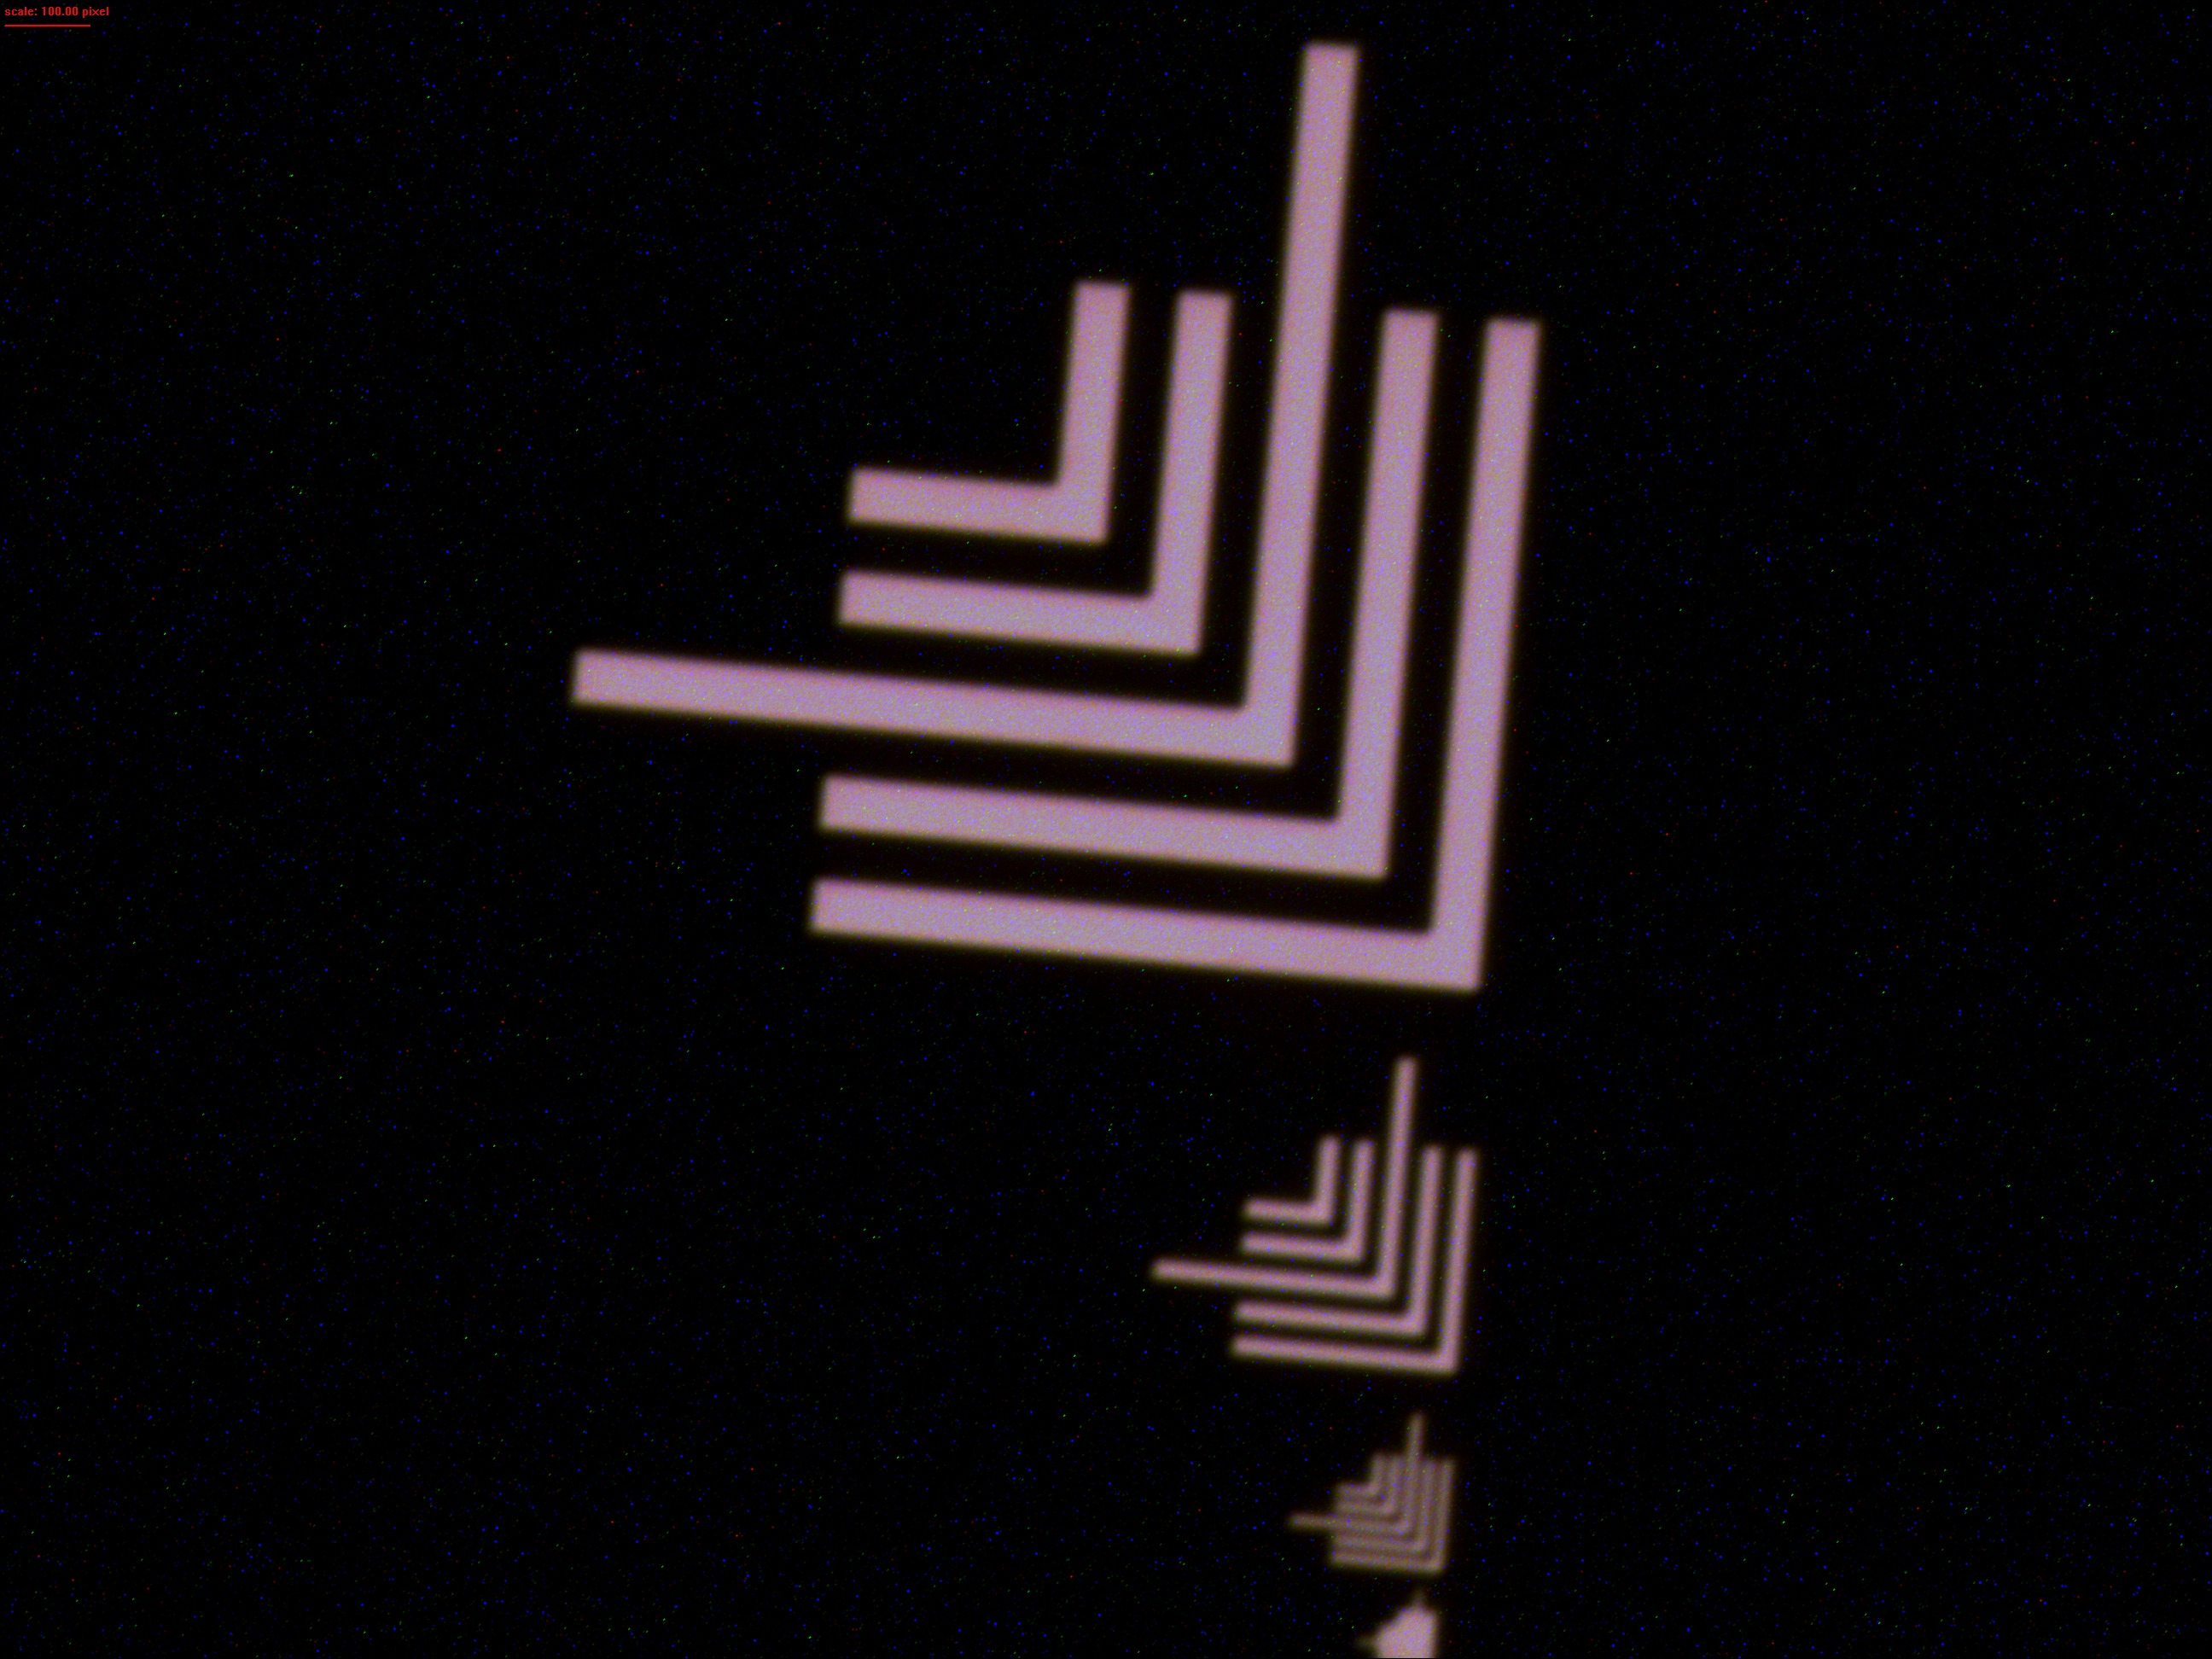
\includegraphics{data/mask/TS_05_20_13_55_57.jpg}}
      	\caption{Zoom in on the previous image.}
      	\label{fig:TS_05_20_13_55_57}
    \end{subfigure}
    \hfill
    \begin{subfigure}[t]{0.24\linewidth}
      	\resizebox{\linewidth}{!}{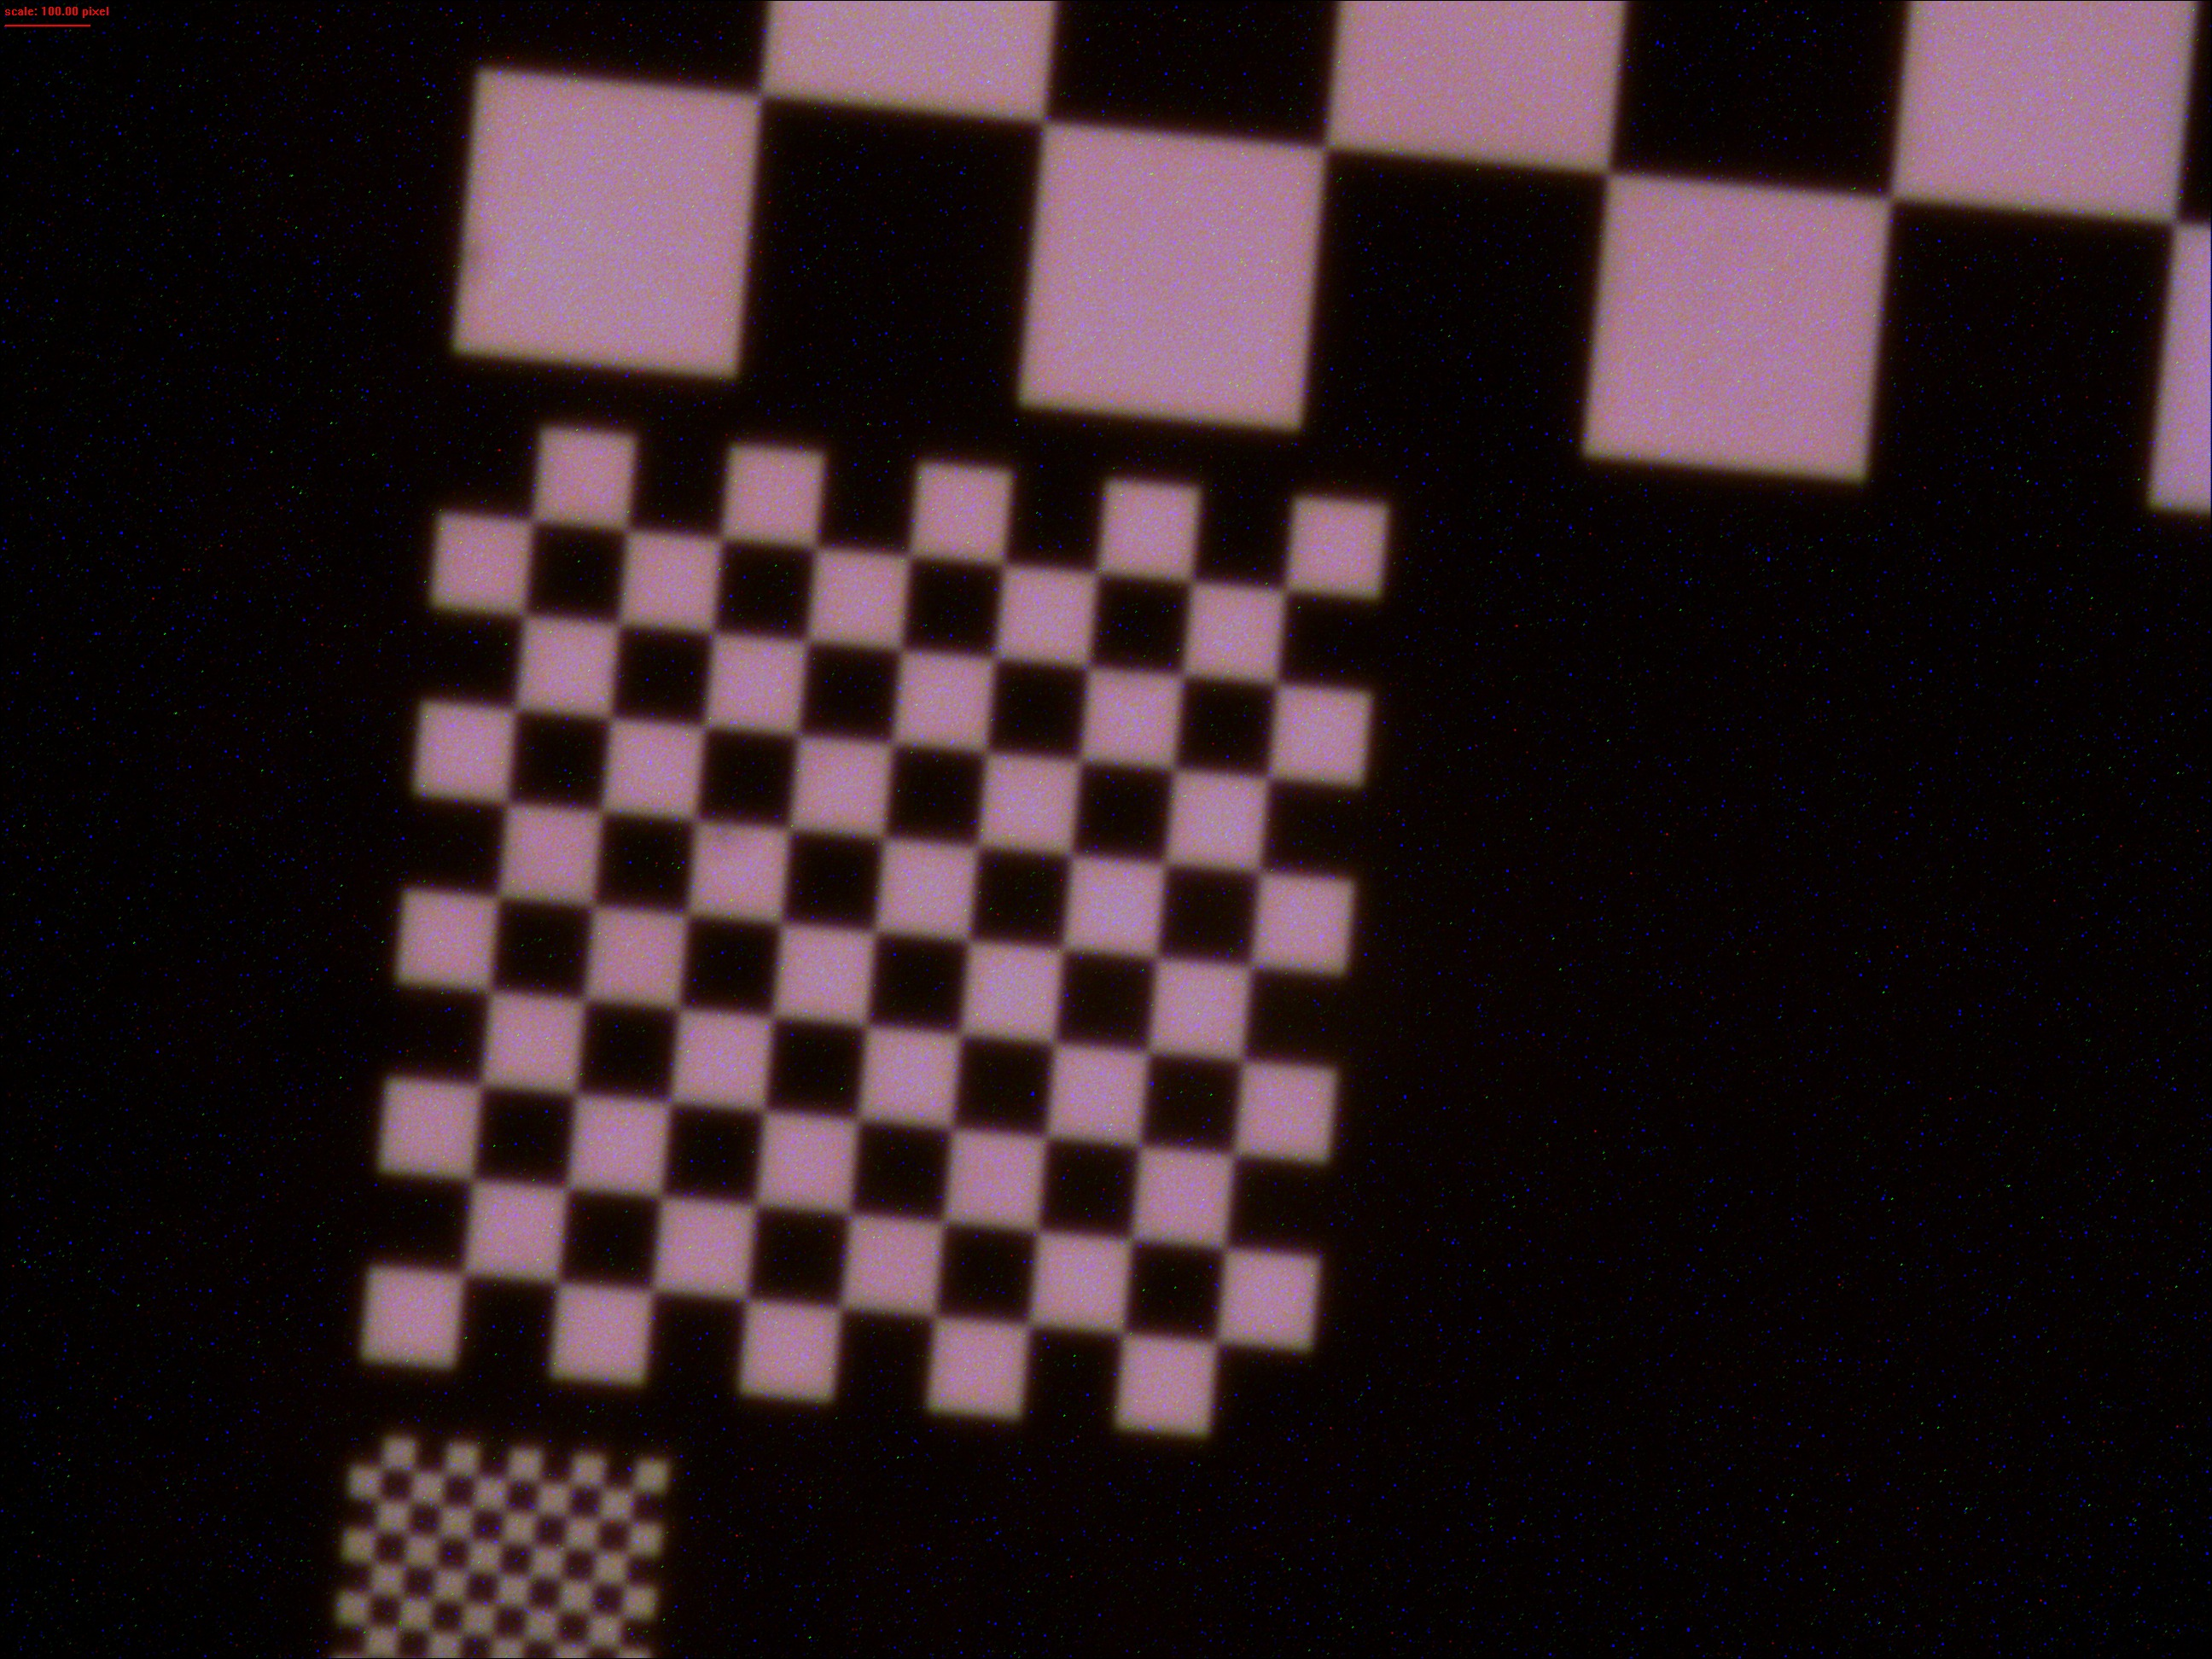
\includegraphics{data/mask/TS_05_20_13_51_30.jpg}}
      	\caption{Checkerboard pattern at several length scales.}
  	    \label{fig:TS_05_20_13_51_30}
    \end{subfigure}
    \hfill
    \begin{subfigure}[t]{0.24\linewidth}
  	    \resizebox{\linewidth}{!}{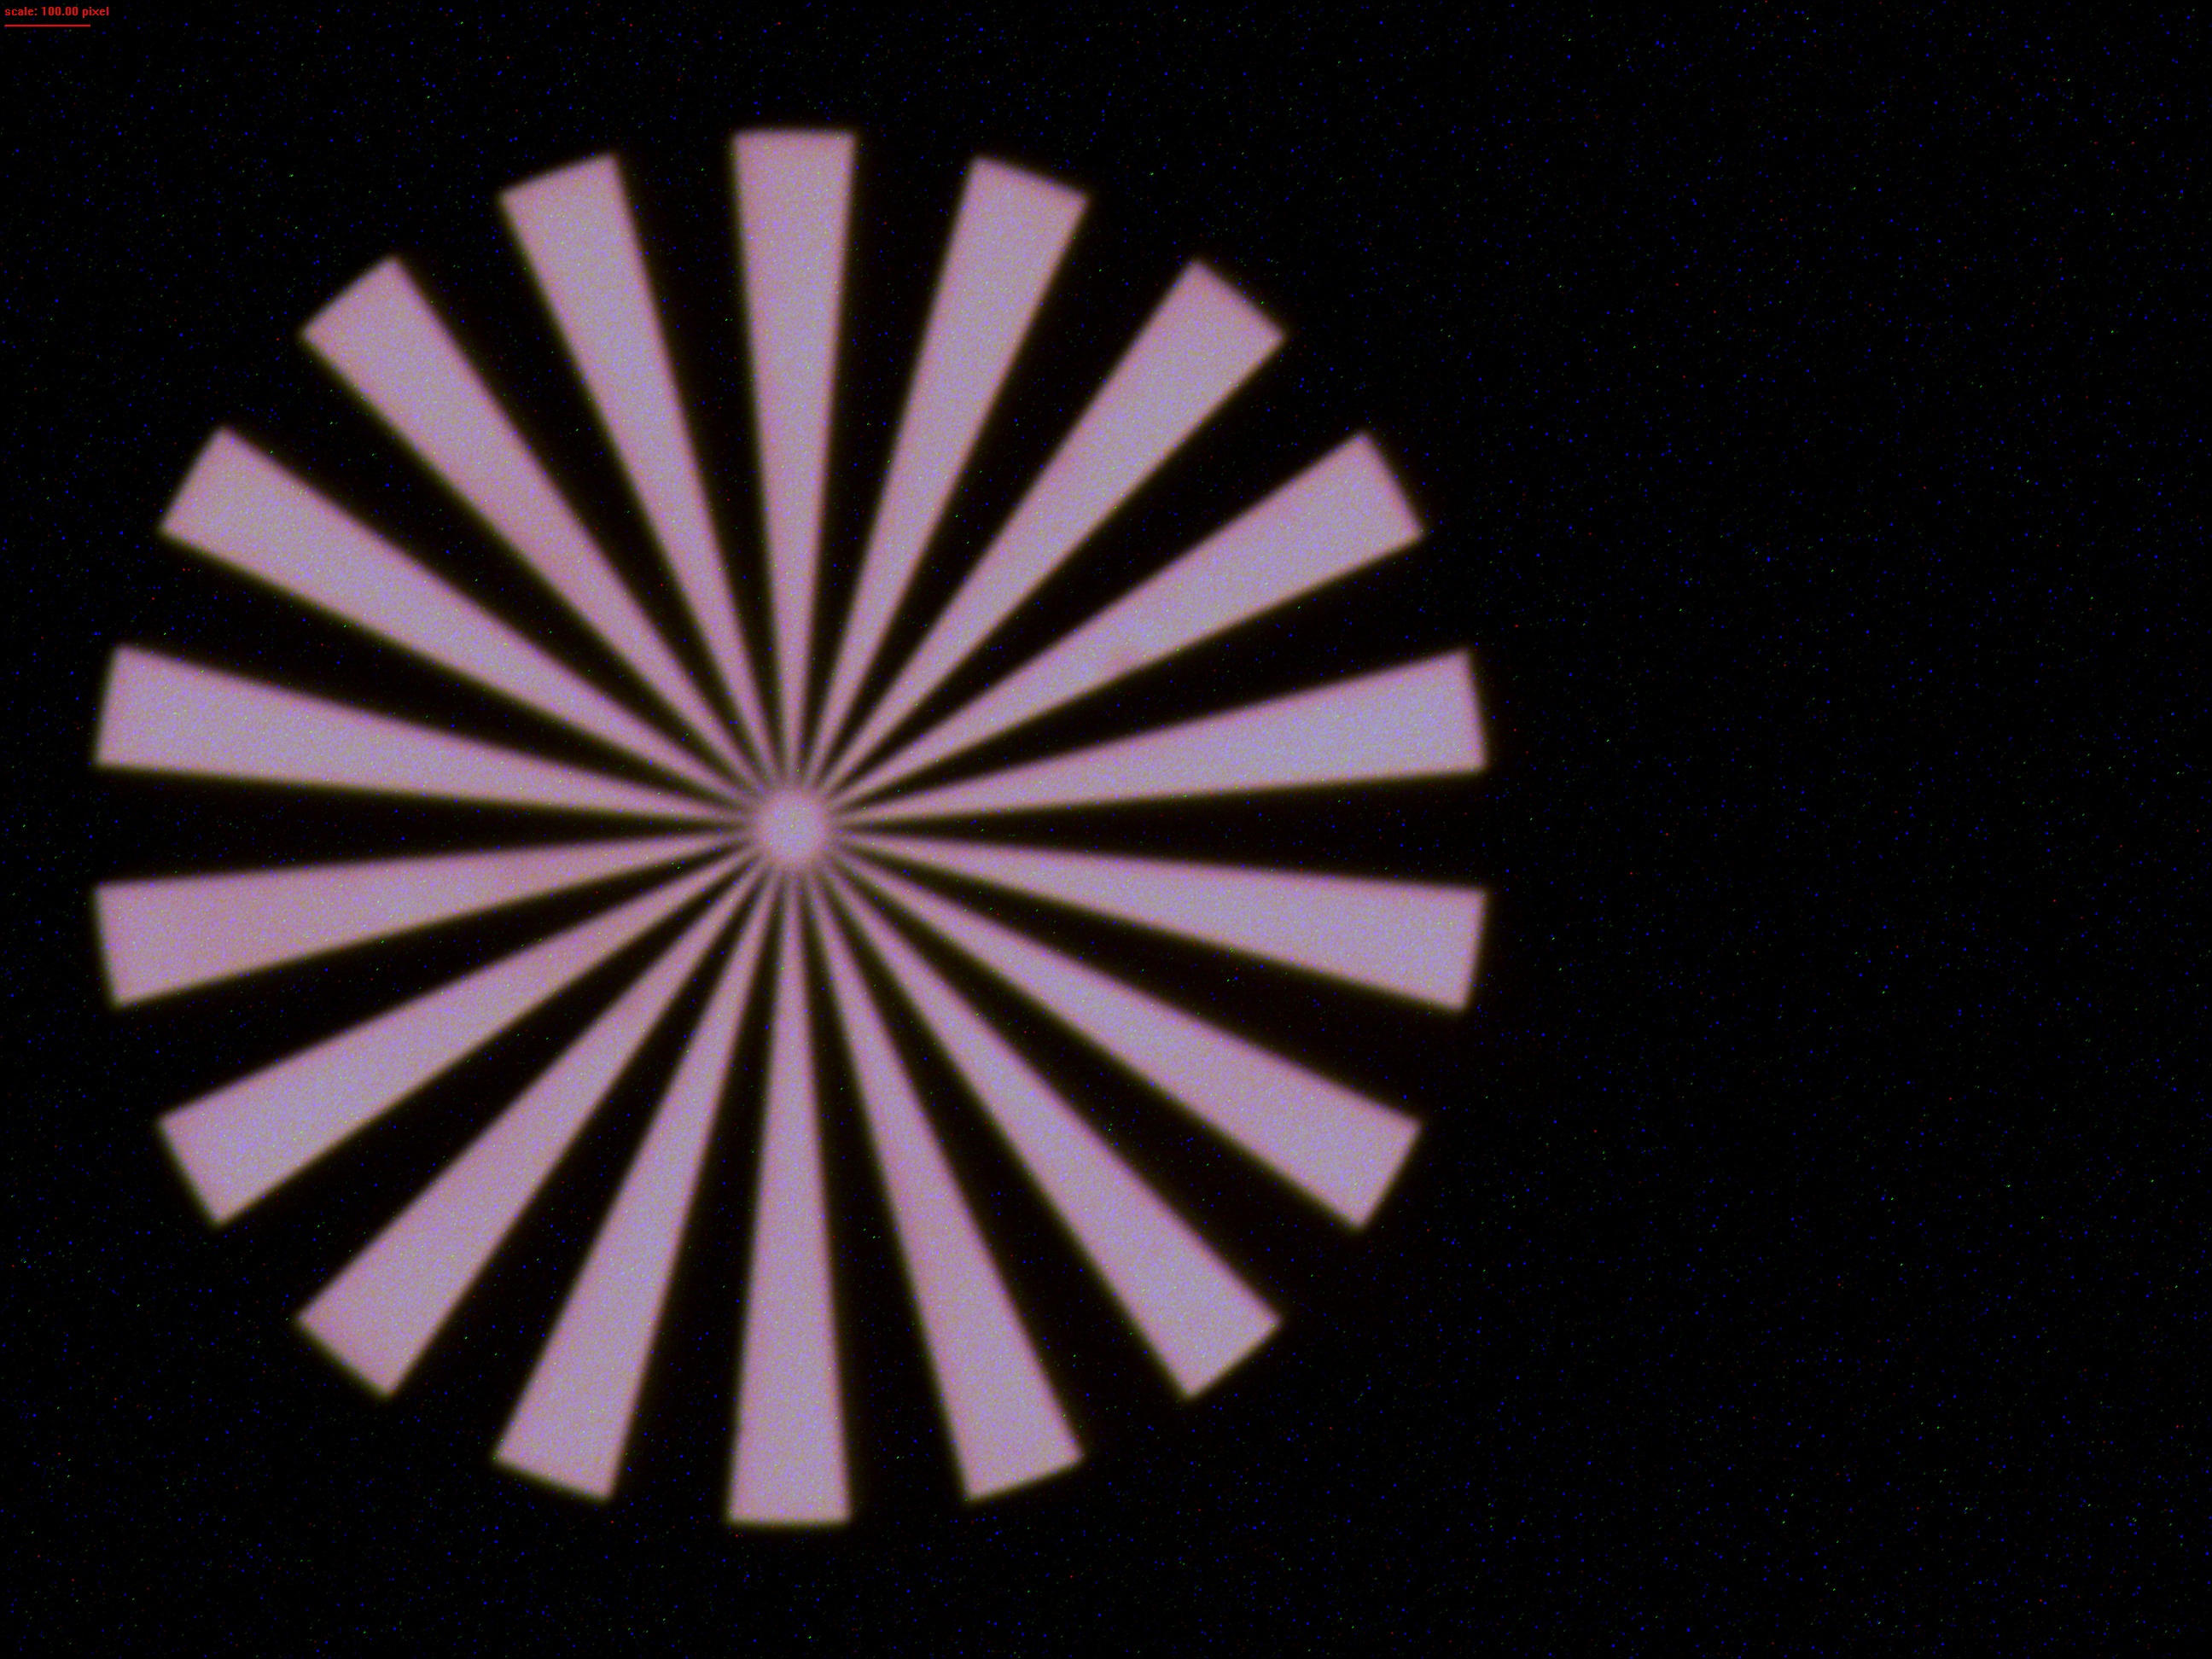
\includegraphics{data/mask/TS_05_20_13_52_44.jpg}}
  	    \caption{Outward radiating lines}
  	    \label{fig:TS_05_20_13_52_44}
    \end{subfigure}
    \hfill
    \begin{subfigure}[t]{0.24\linewidth}
      	\resizebox{\linewidth}{!}{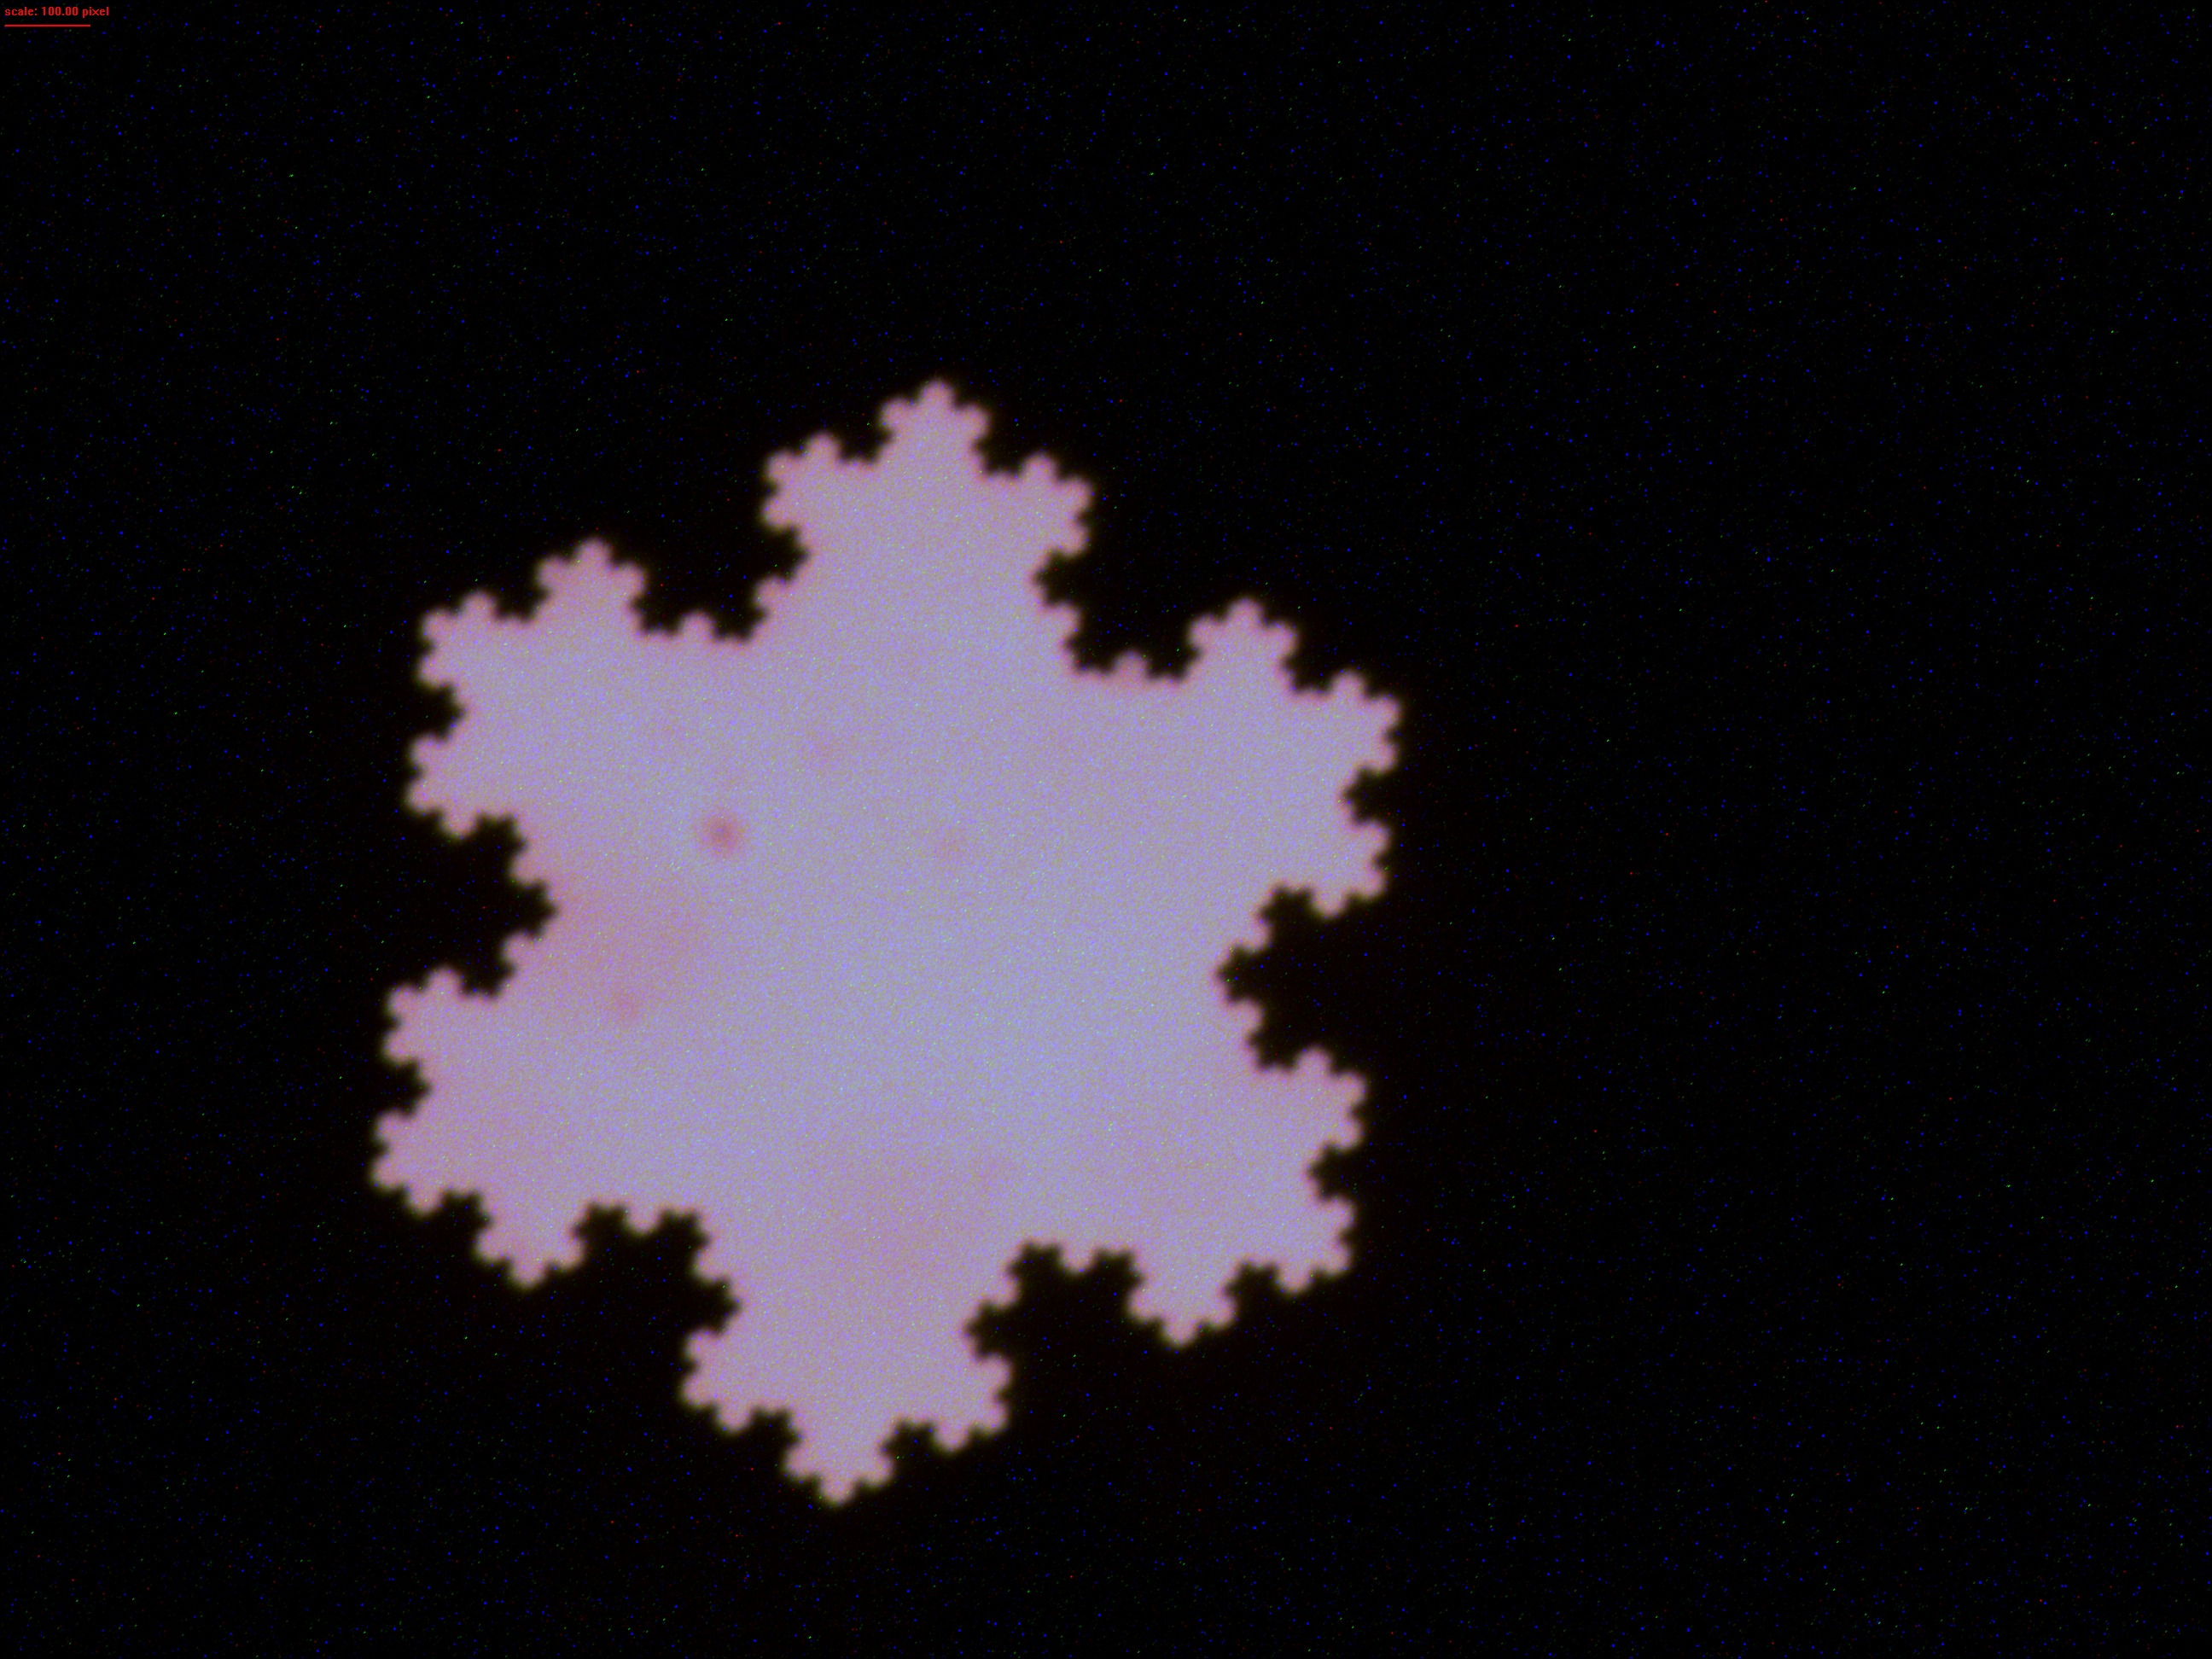
\includegraphics{data/mask/TS_05_20_13_53_38.jpg}}
      	\caption{Koch snowflake.}
      	\label{fig:TS_05_20_13_53_38}
    \end{subfigure}
    \hfill
    \begin{subfigure}[t]{0.24\linewidth}
      	\resizebox{\linewidth}{!}{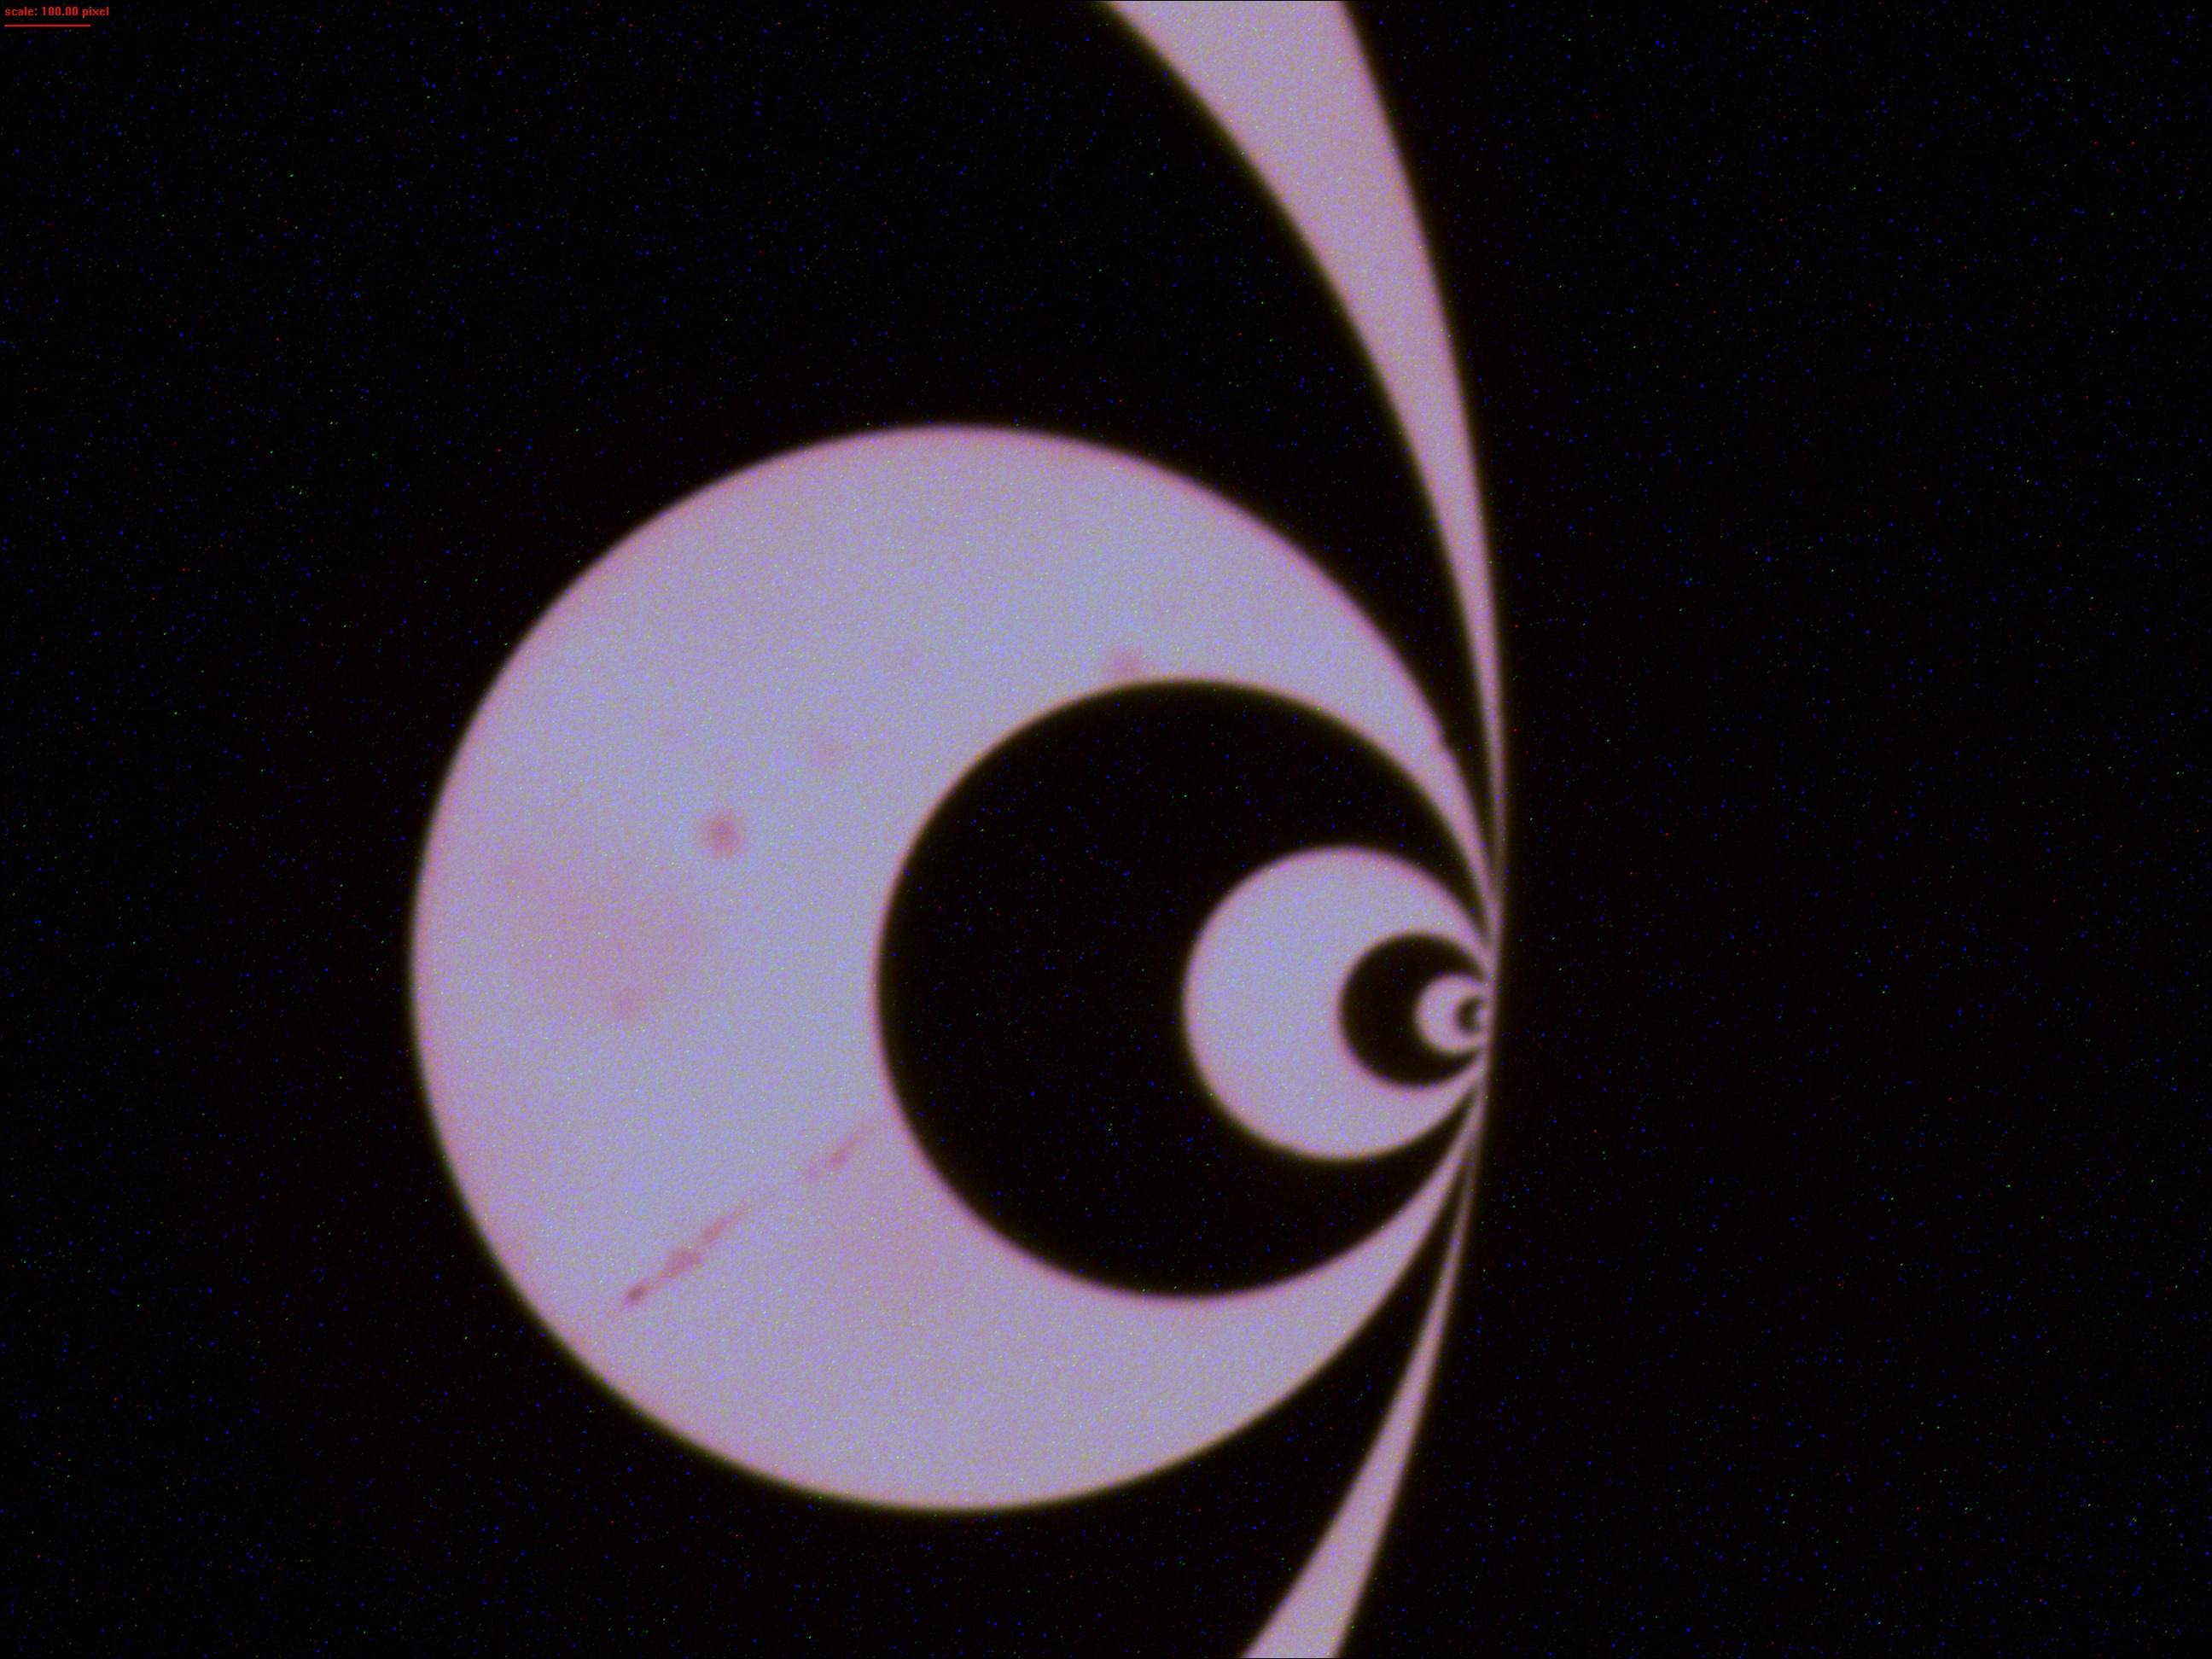
\includegraphics{data/mask/TS_05_20_13_54_28.jpg}}
      	\caption{Internally touching circles.}
      	\label{fig:TS_05_20_13_54_28}
    \end{subfigure}
    \hfill
    \begin{subfigure}[t]{0.24\linewidth}
      	\resizebox{\linewidth}{!}{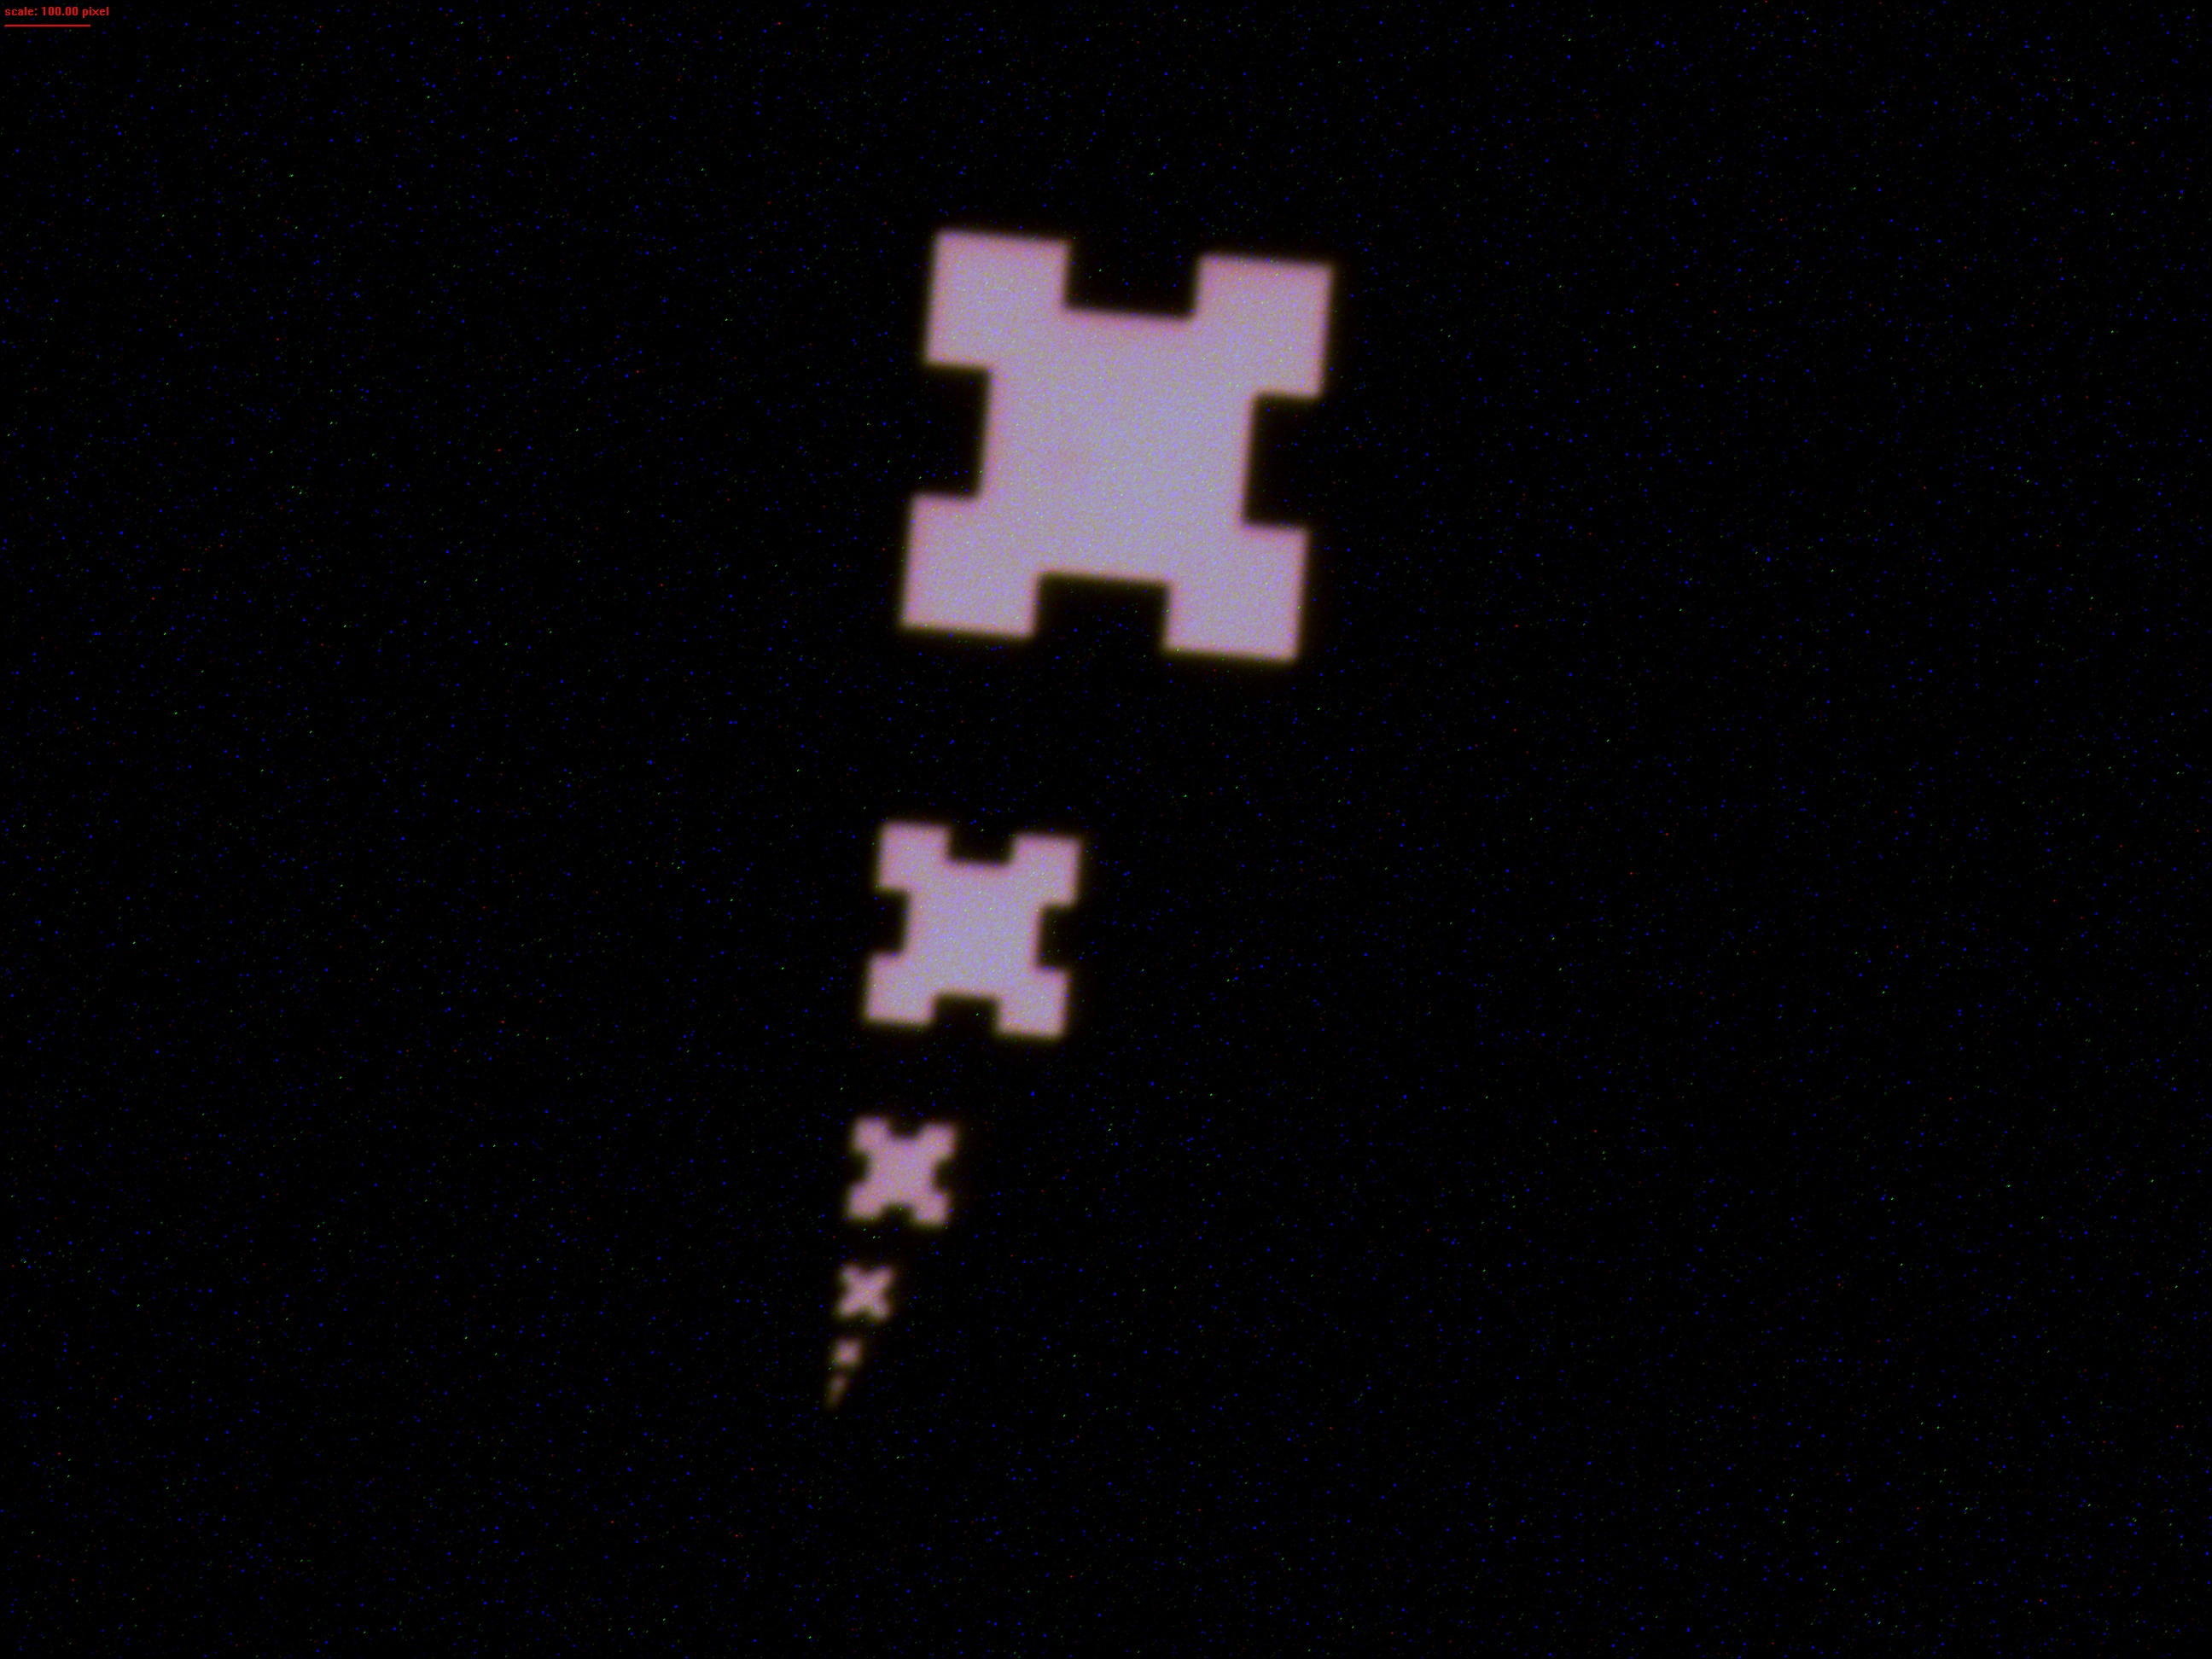
\includegraphics{data/mask/TS_05_20_13_54_51.jpg}}
      	\caption{Squares with OPC patterns.}
      	\label{fig:TS_05_20_13_54_51}
    \end{subfigure}
    \caption{Optical microscope images of some parts of the photomask. Images were taken in transmission mode.}
\end{figure*}

\begin{figure*}[htb]
    \centering
    % \begin{subfigure}[t]{0.32\linewidth}
 	  %  \resizebox{\linewidth}{!}{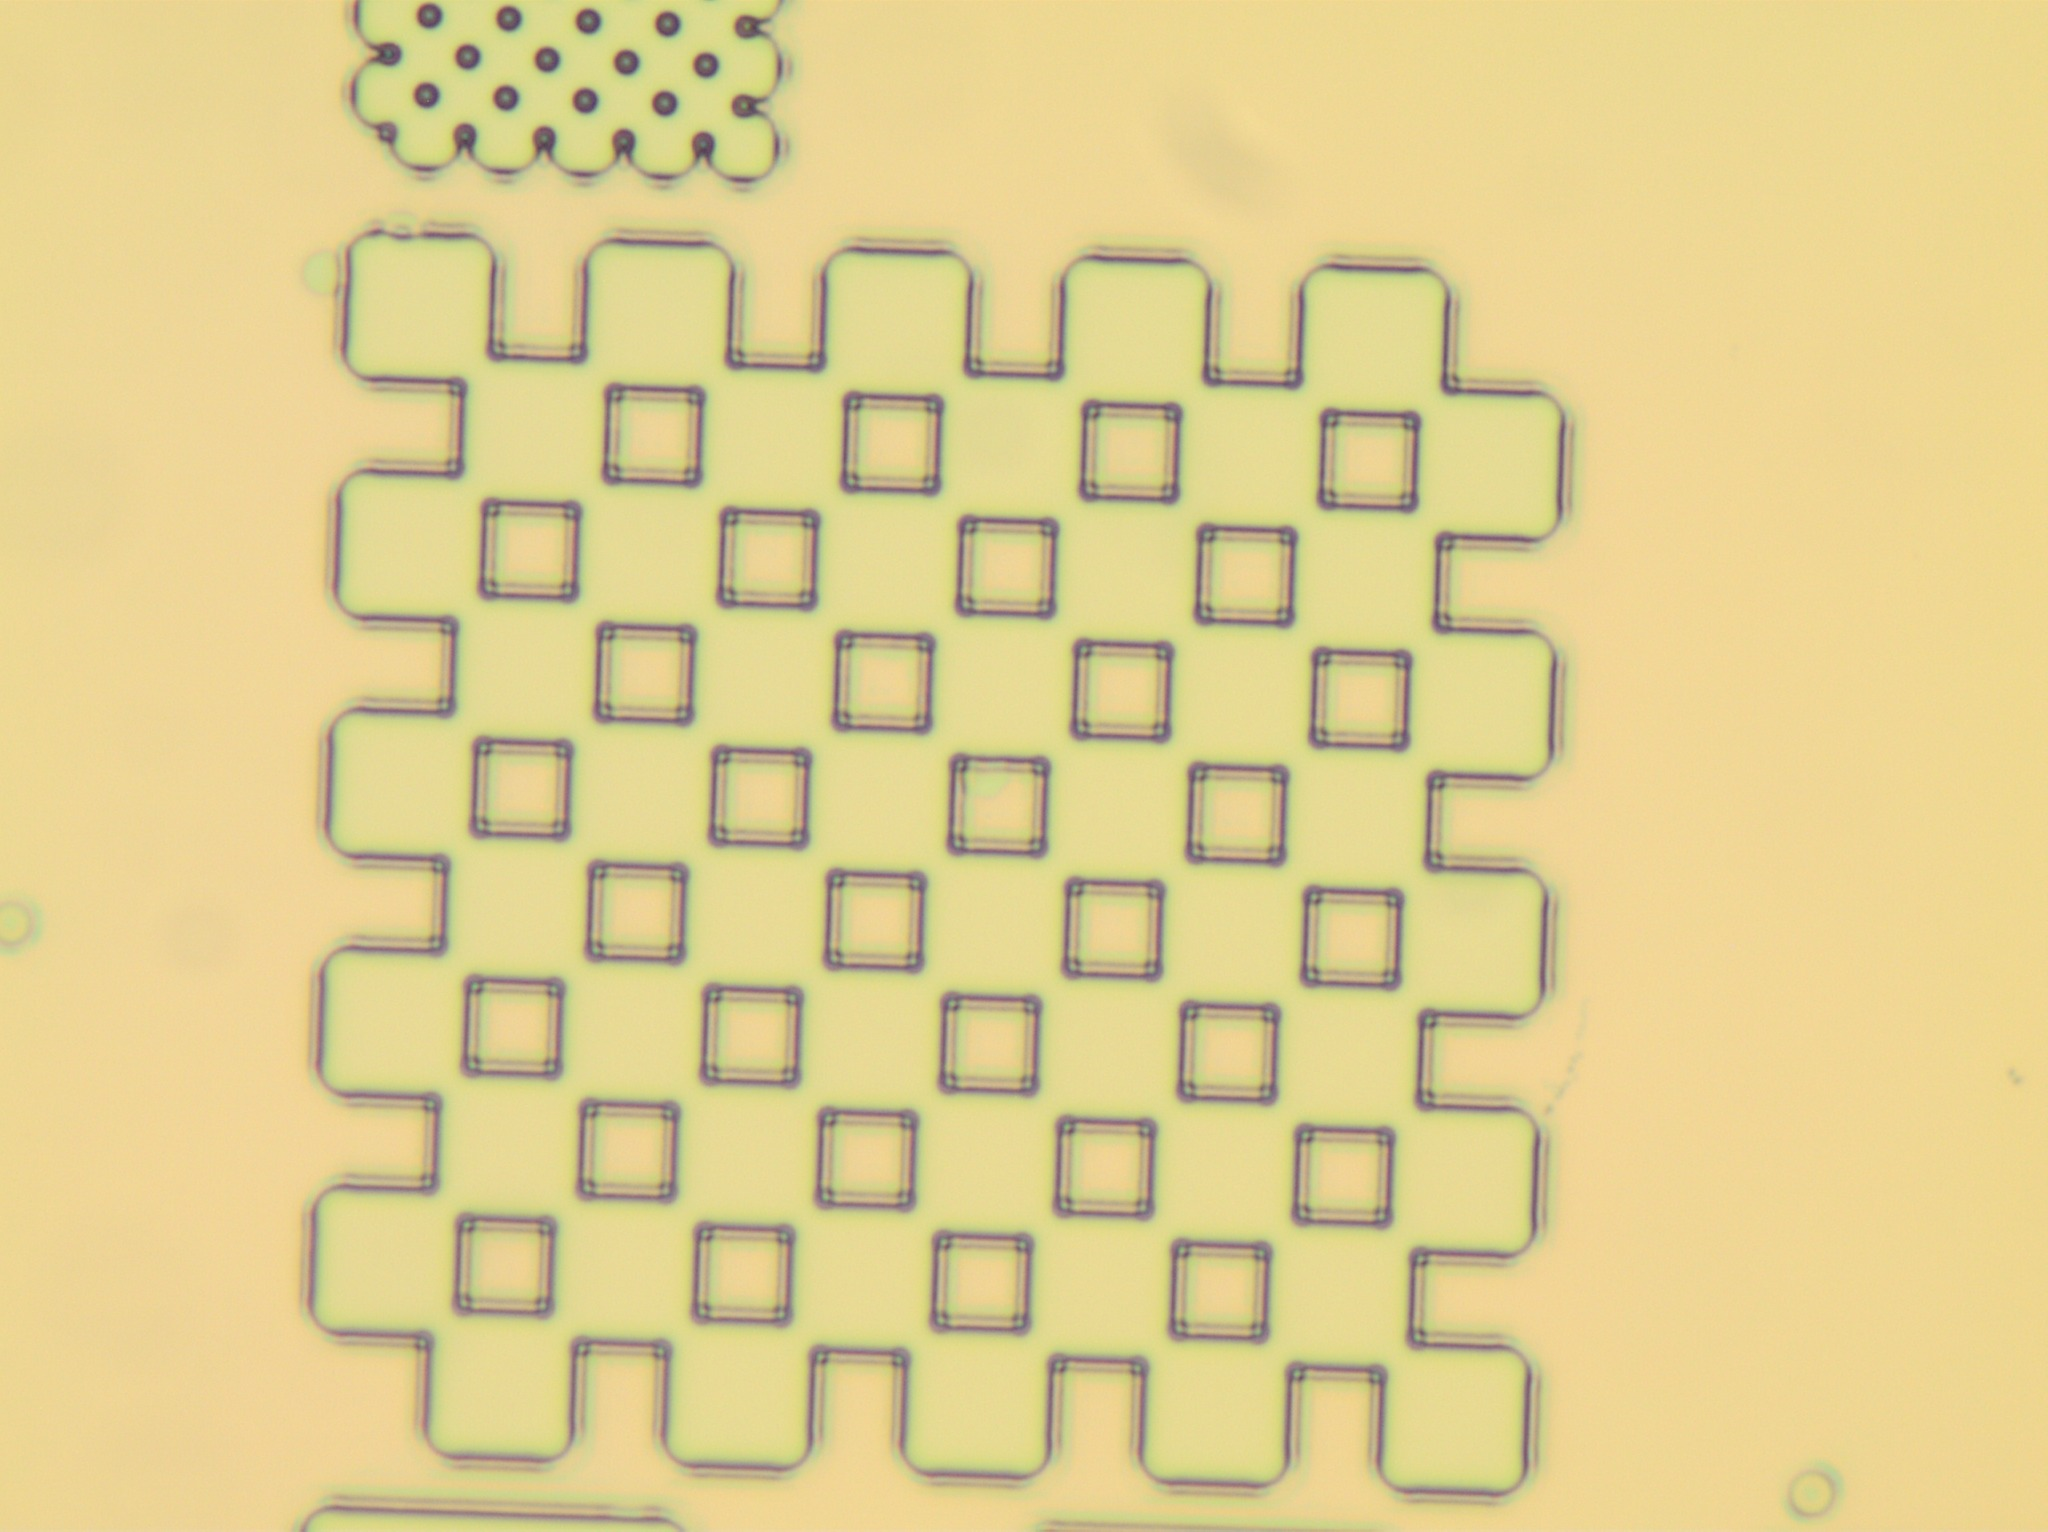
\includegraphics{data/b3d1.jpg}}
  	 %   \caption{Exposure time of 1.0 minutes}
  	 %   \label{fig:b3d1}
    % \end{subfigure}
    % \hfill
    % \begin{subfigure}[t]{0.32\linewidth}
 	  %  \resizebox{\linewidth}{!}{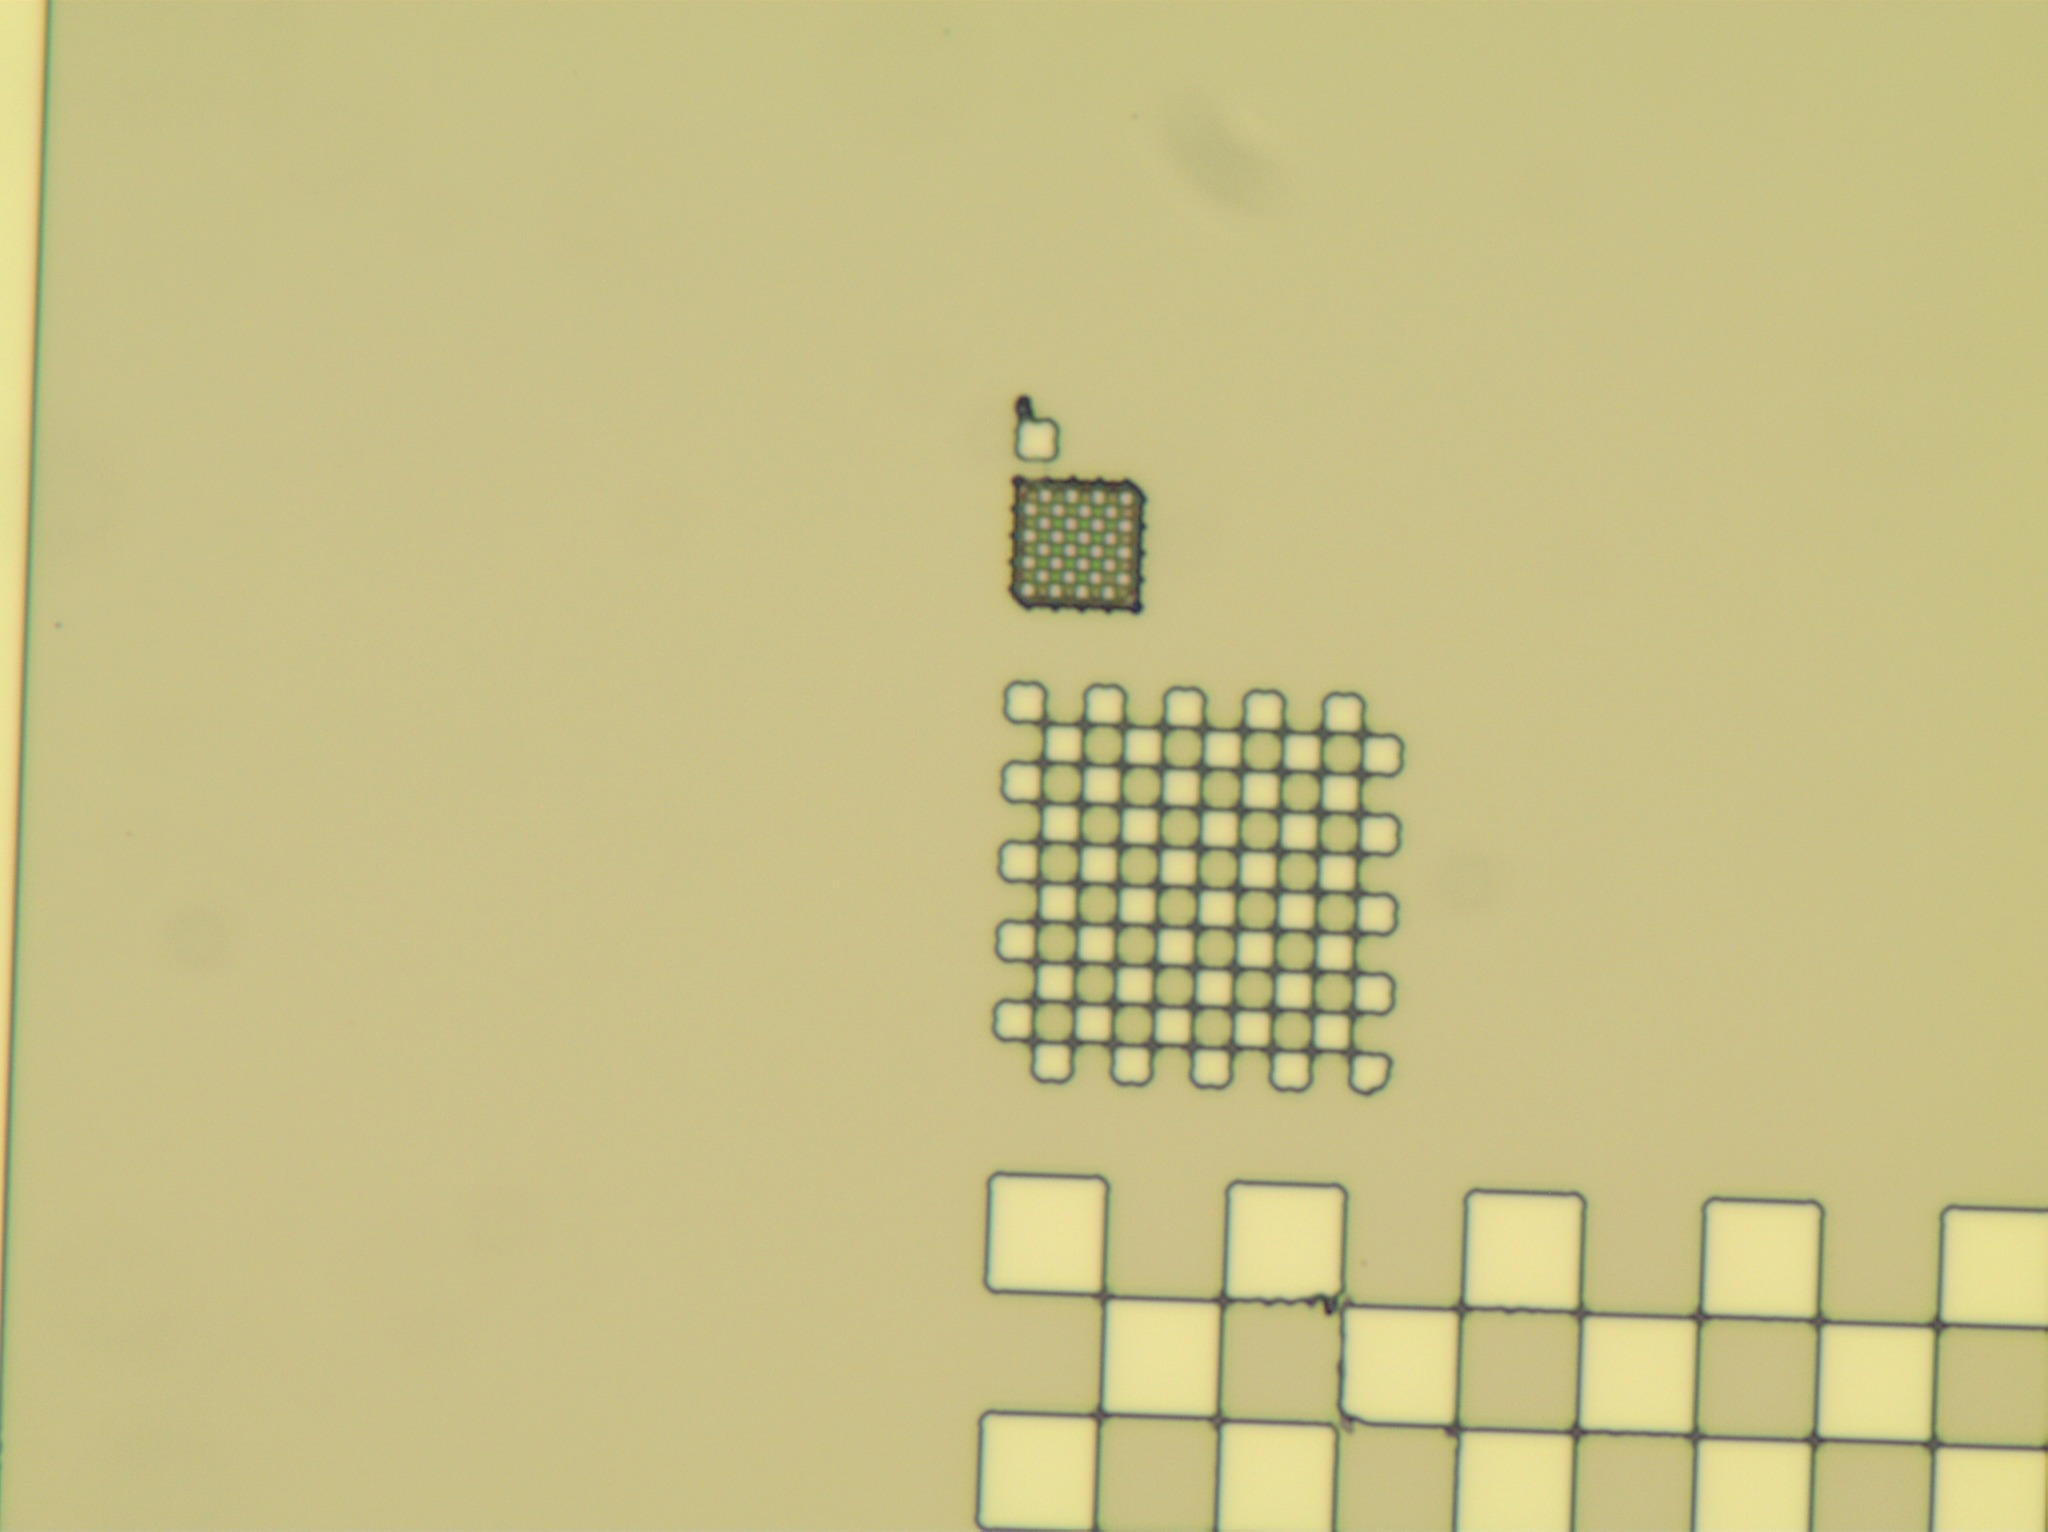
\includegraphics{data/b3a1.jpg}}
  	 %   \caption{Exposure time of 2.0 minutes}
  	 %   \label{fig:b3a1}
    % \end{subfigure}
    % \hfill
    % \begin{subfigure}[t]{0.32\linewidth}
 	  %  \resizebox{\linewidth}{!}{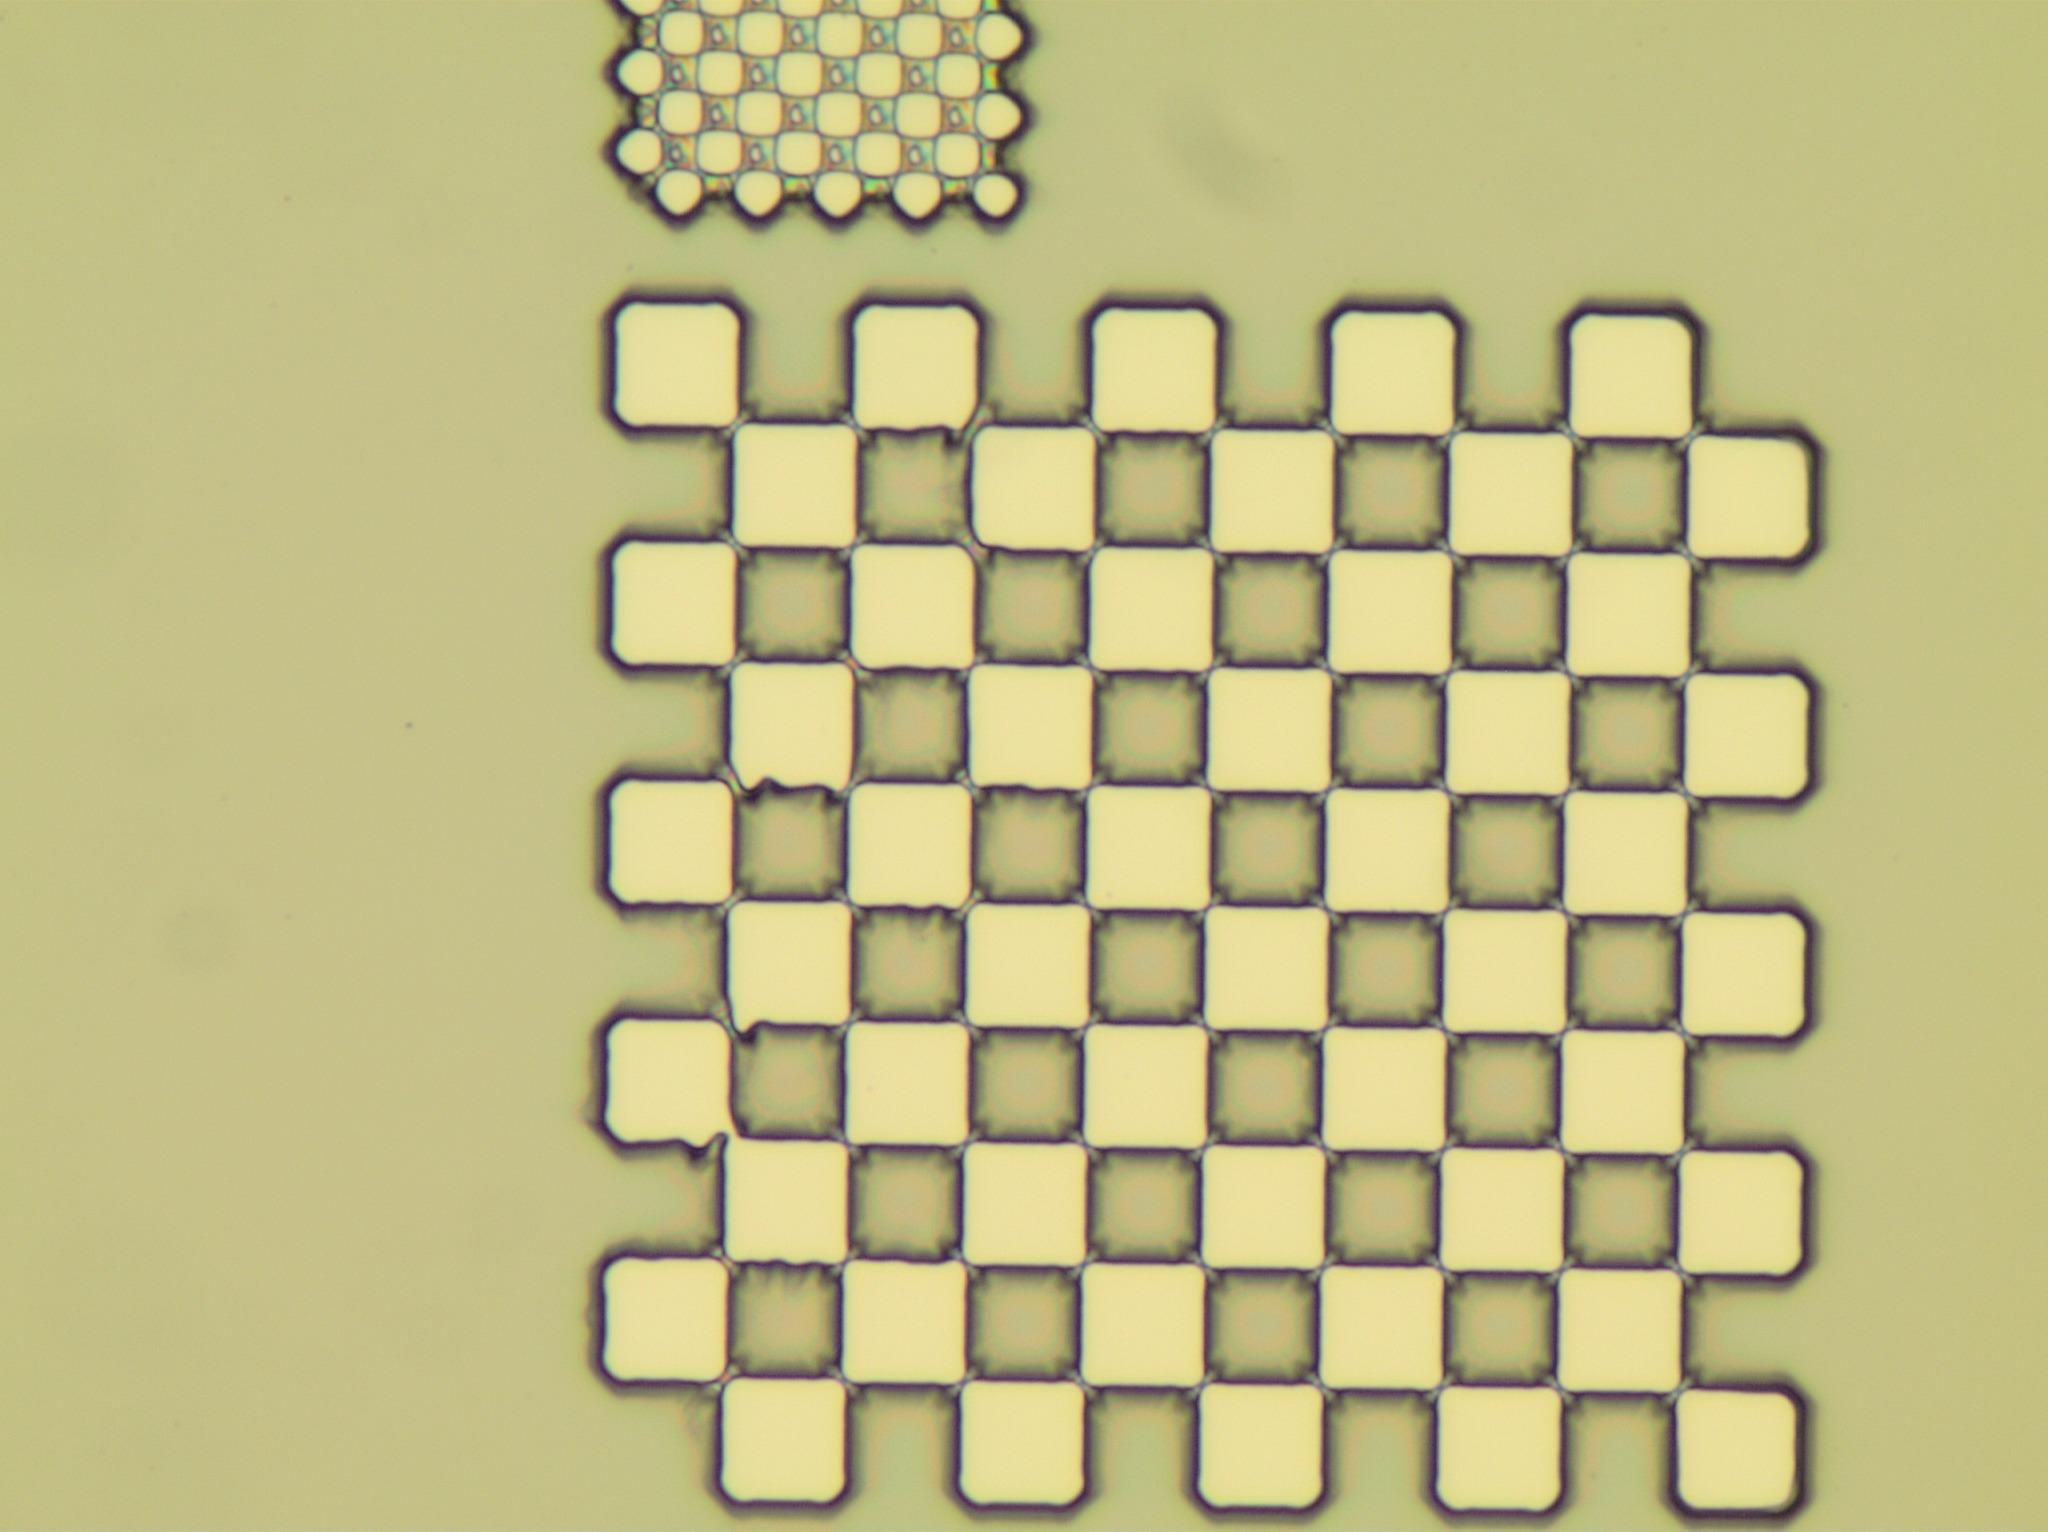
\includegraphics{data/b3e1.jpg}}
  	 %   \caption{Exposure time of 2.5 minutes}
  	 %   \label{fig:b3e1}
    % \end{subfigure}\\
    \begin{subfigure}[t]{0.32\linewidth}
     	\resizebox{\linewidth}{!}{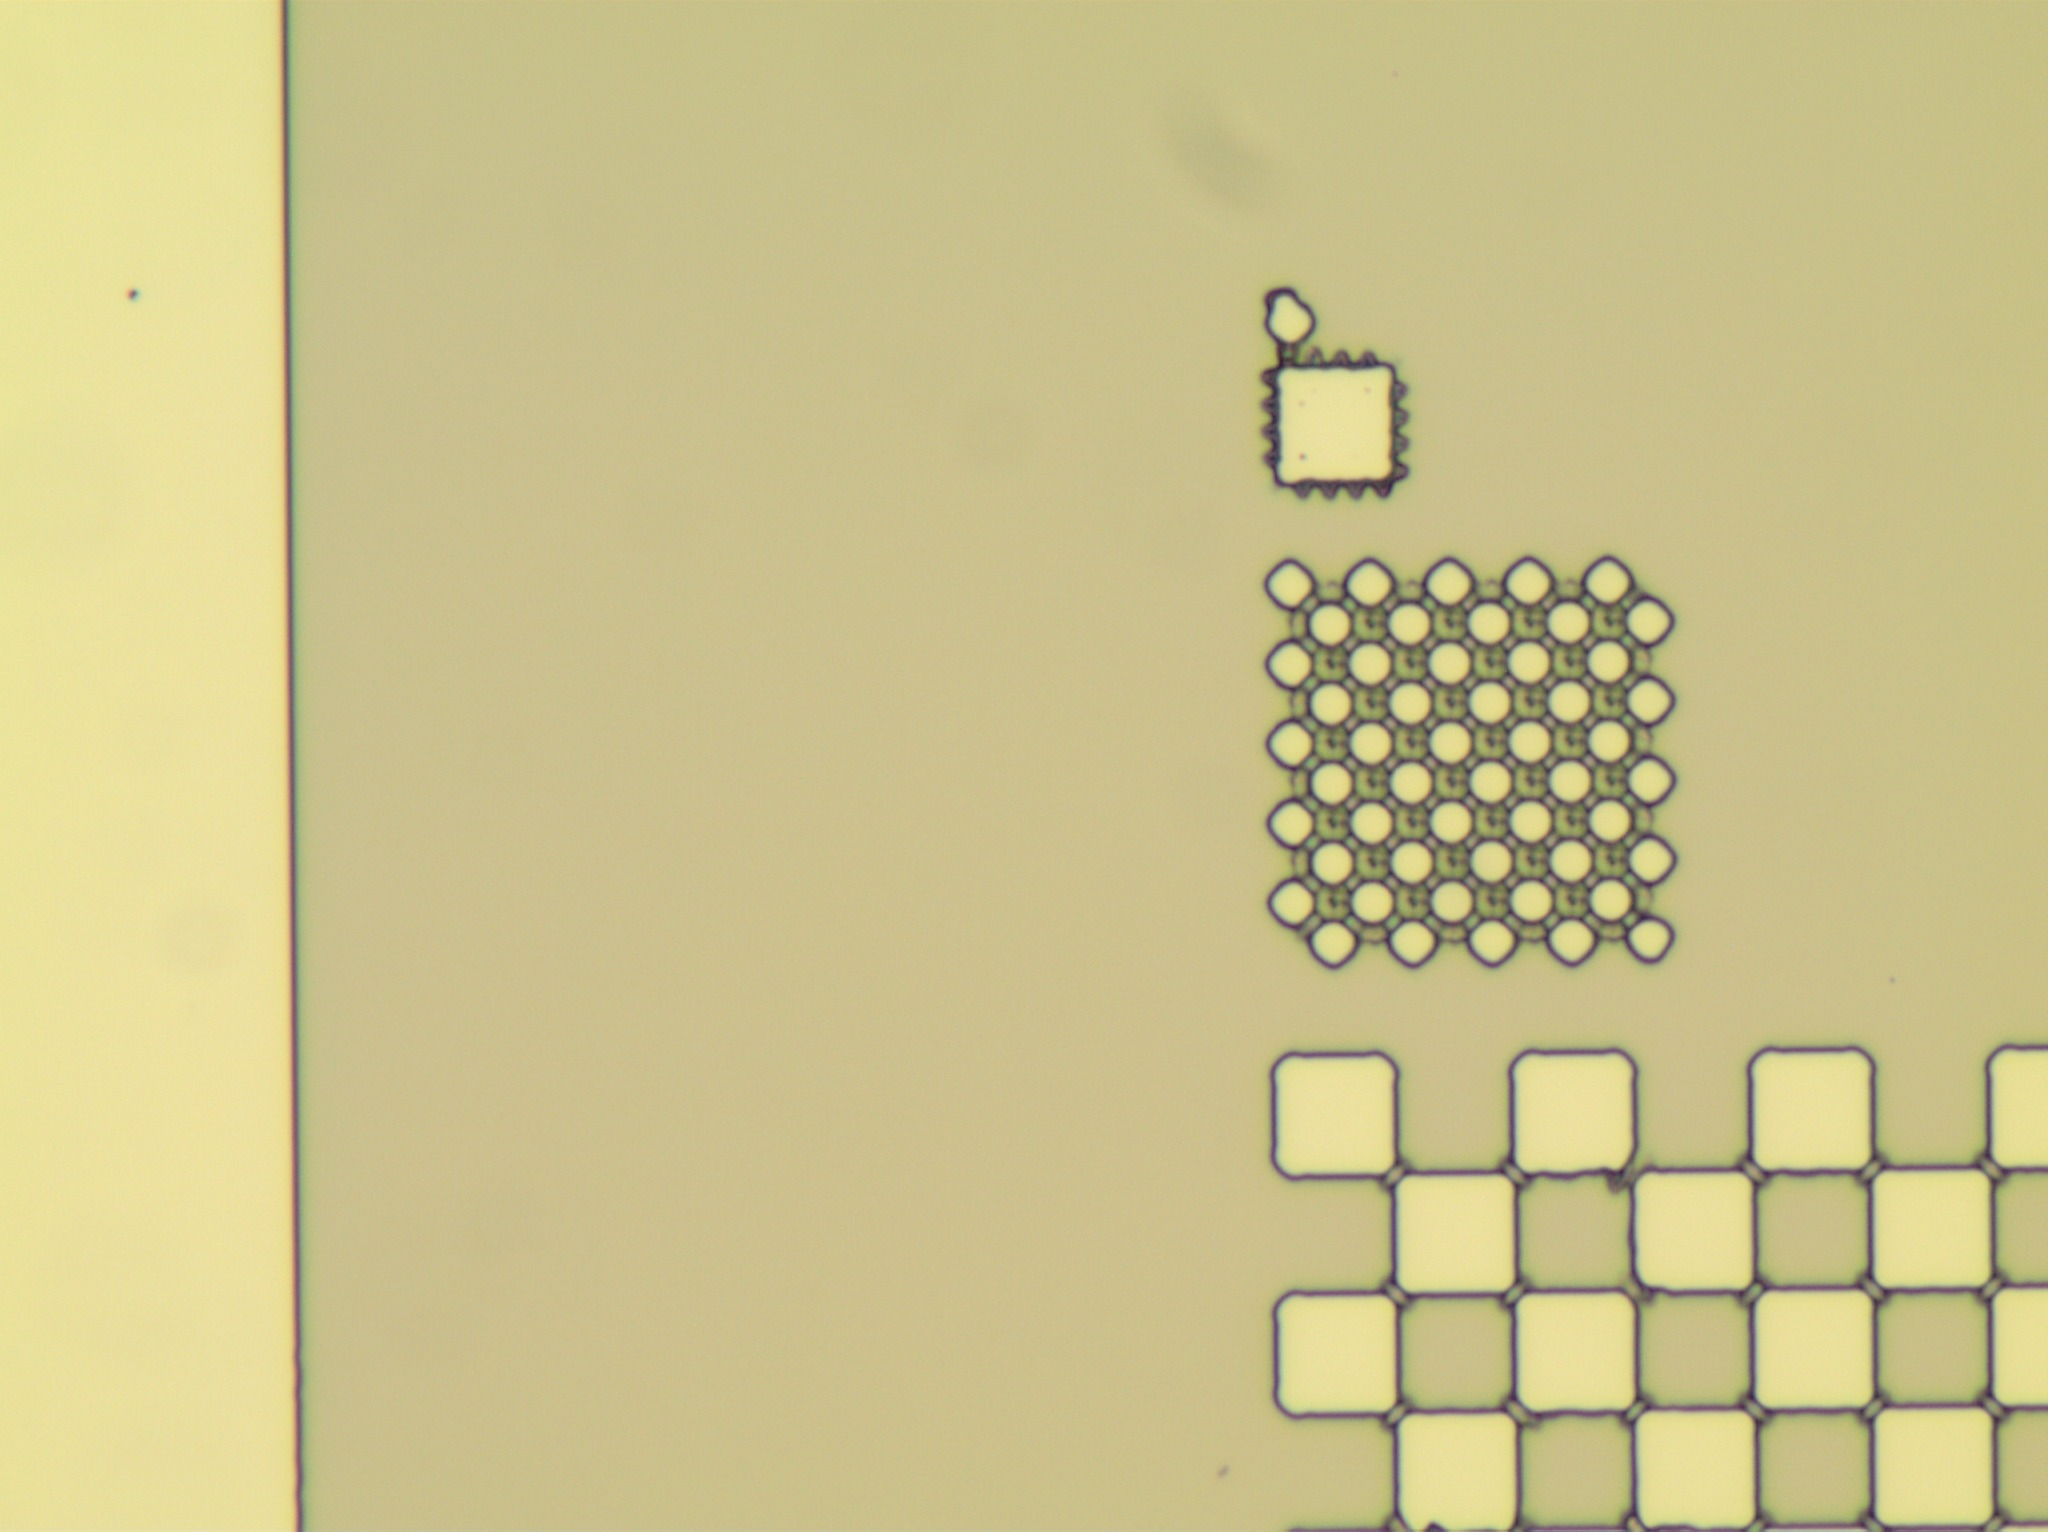
\includegraphics{data/b3b2.jpg}}
      	\caption{Exposure time of 3.0 minutes}
      	\label{fig:b3b2}
    \end{subfigure}
    \hfill
    \begin{subfigure}[t]{0.32\linewidth}
     	\resizebox{\linewidth}{!}{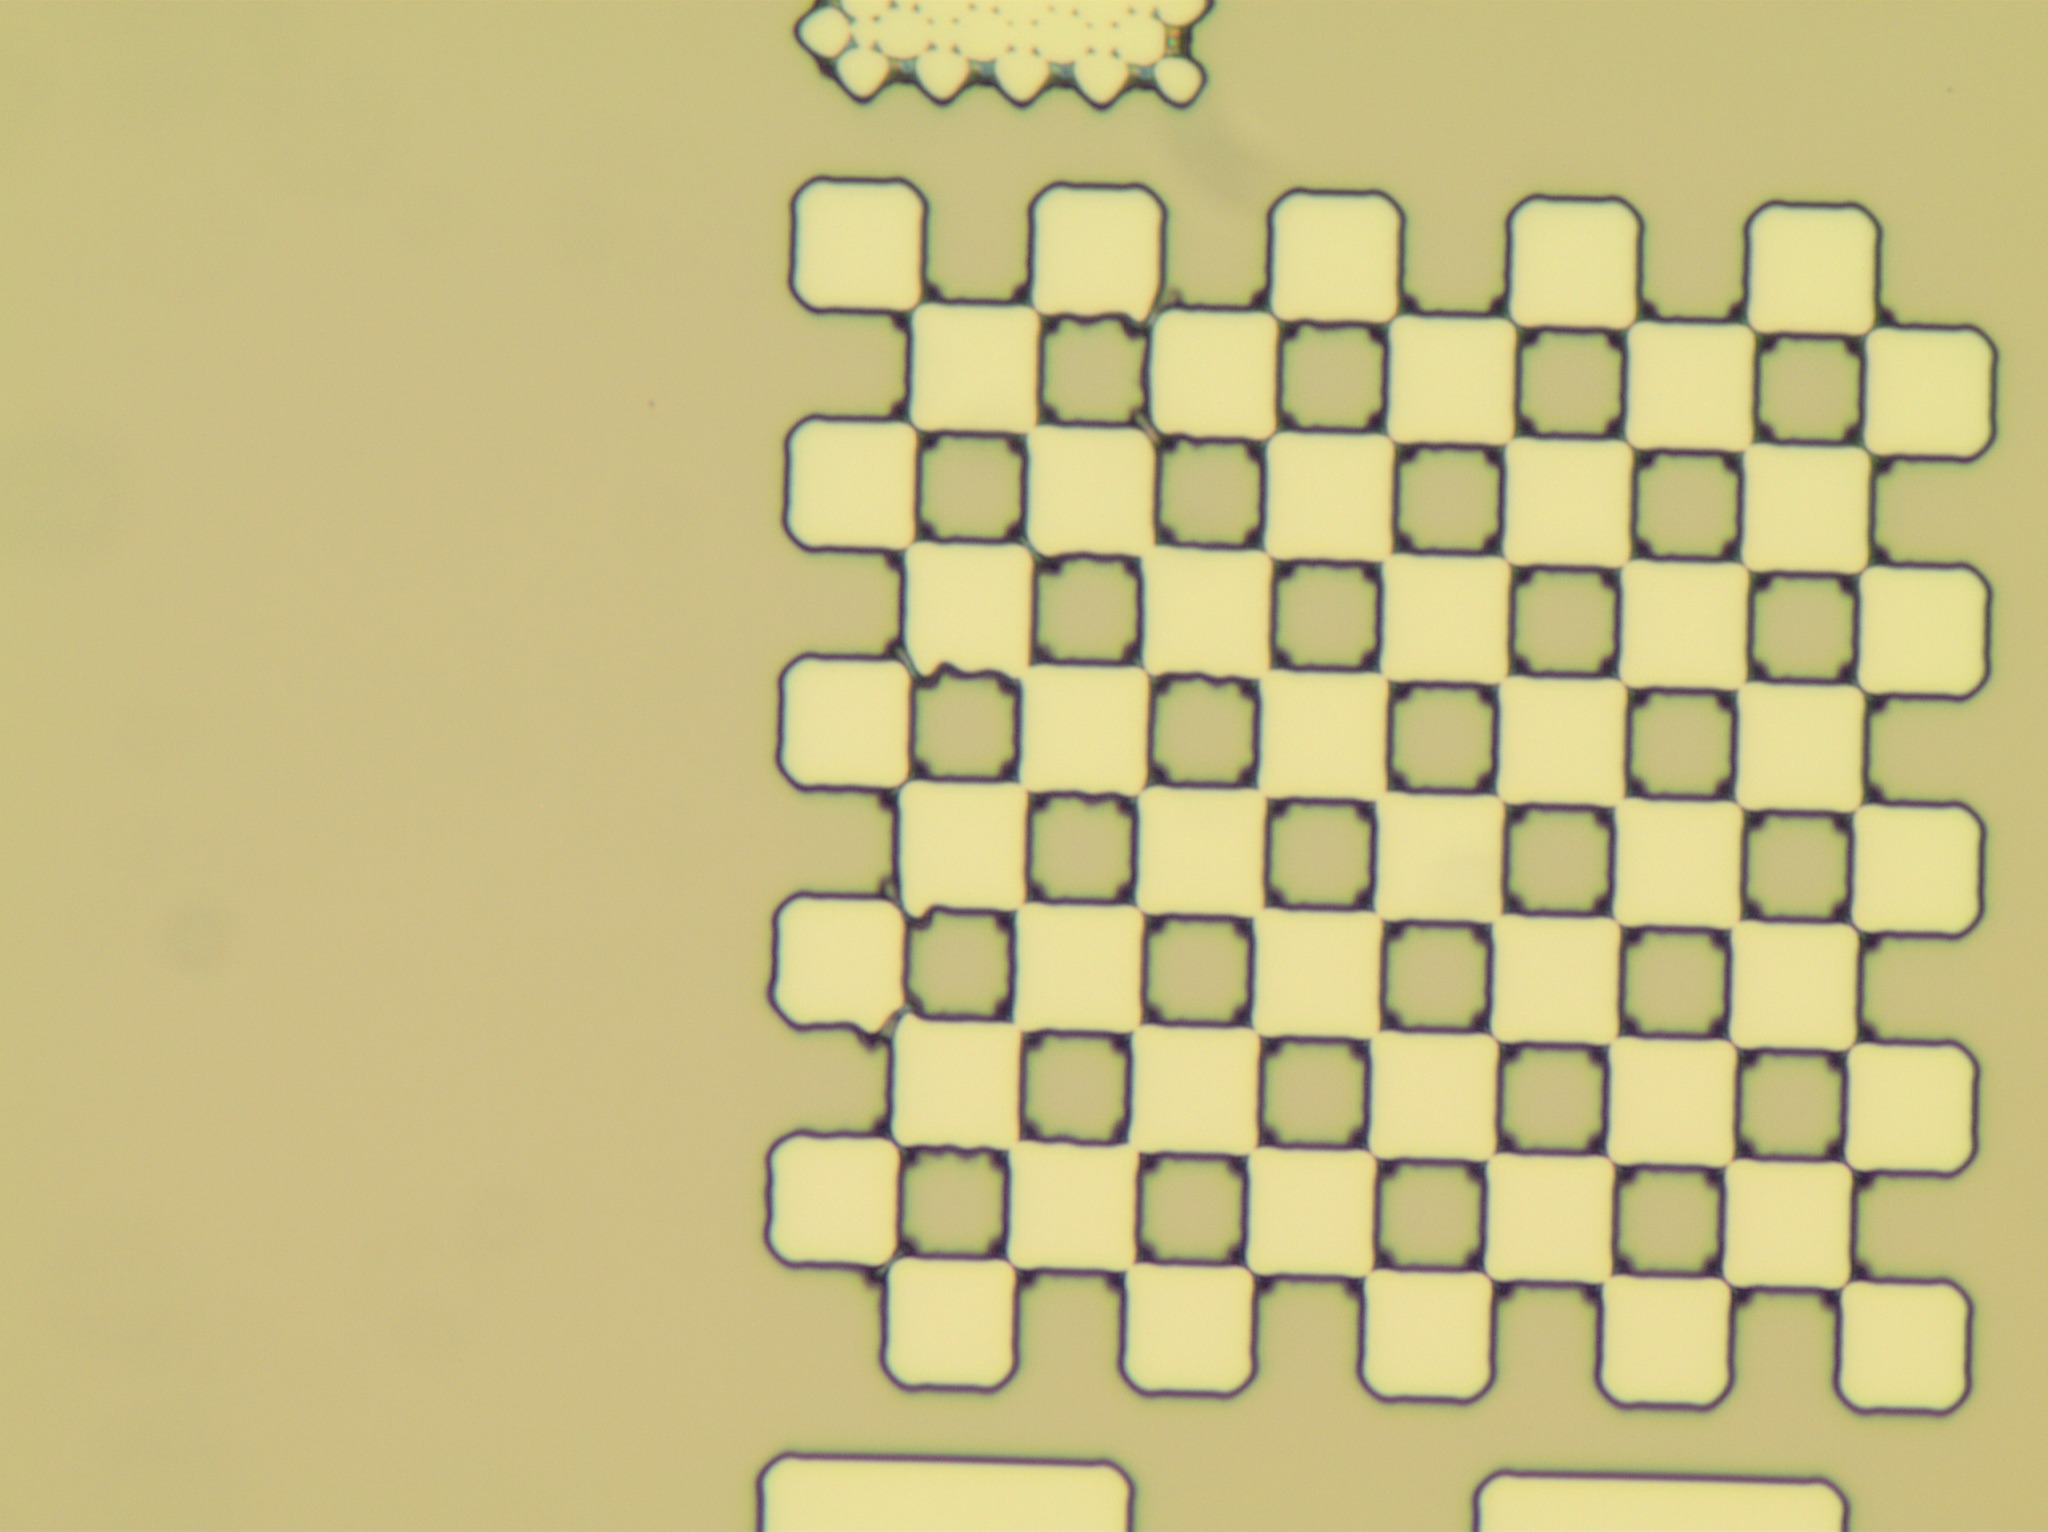
\includegraphics{data/b3c1.jpg}}
      	\caption{Exposure time of 3.5 minutes}
      	\label{fig:b3c1}
    \end{subfigure}
    \hfill
    \begin{subfigure}[t]{0.32\linewidth}
 	    \resizebox{\linewidth}{!}{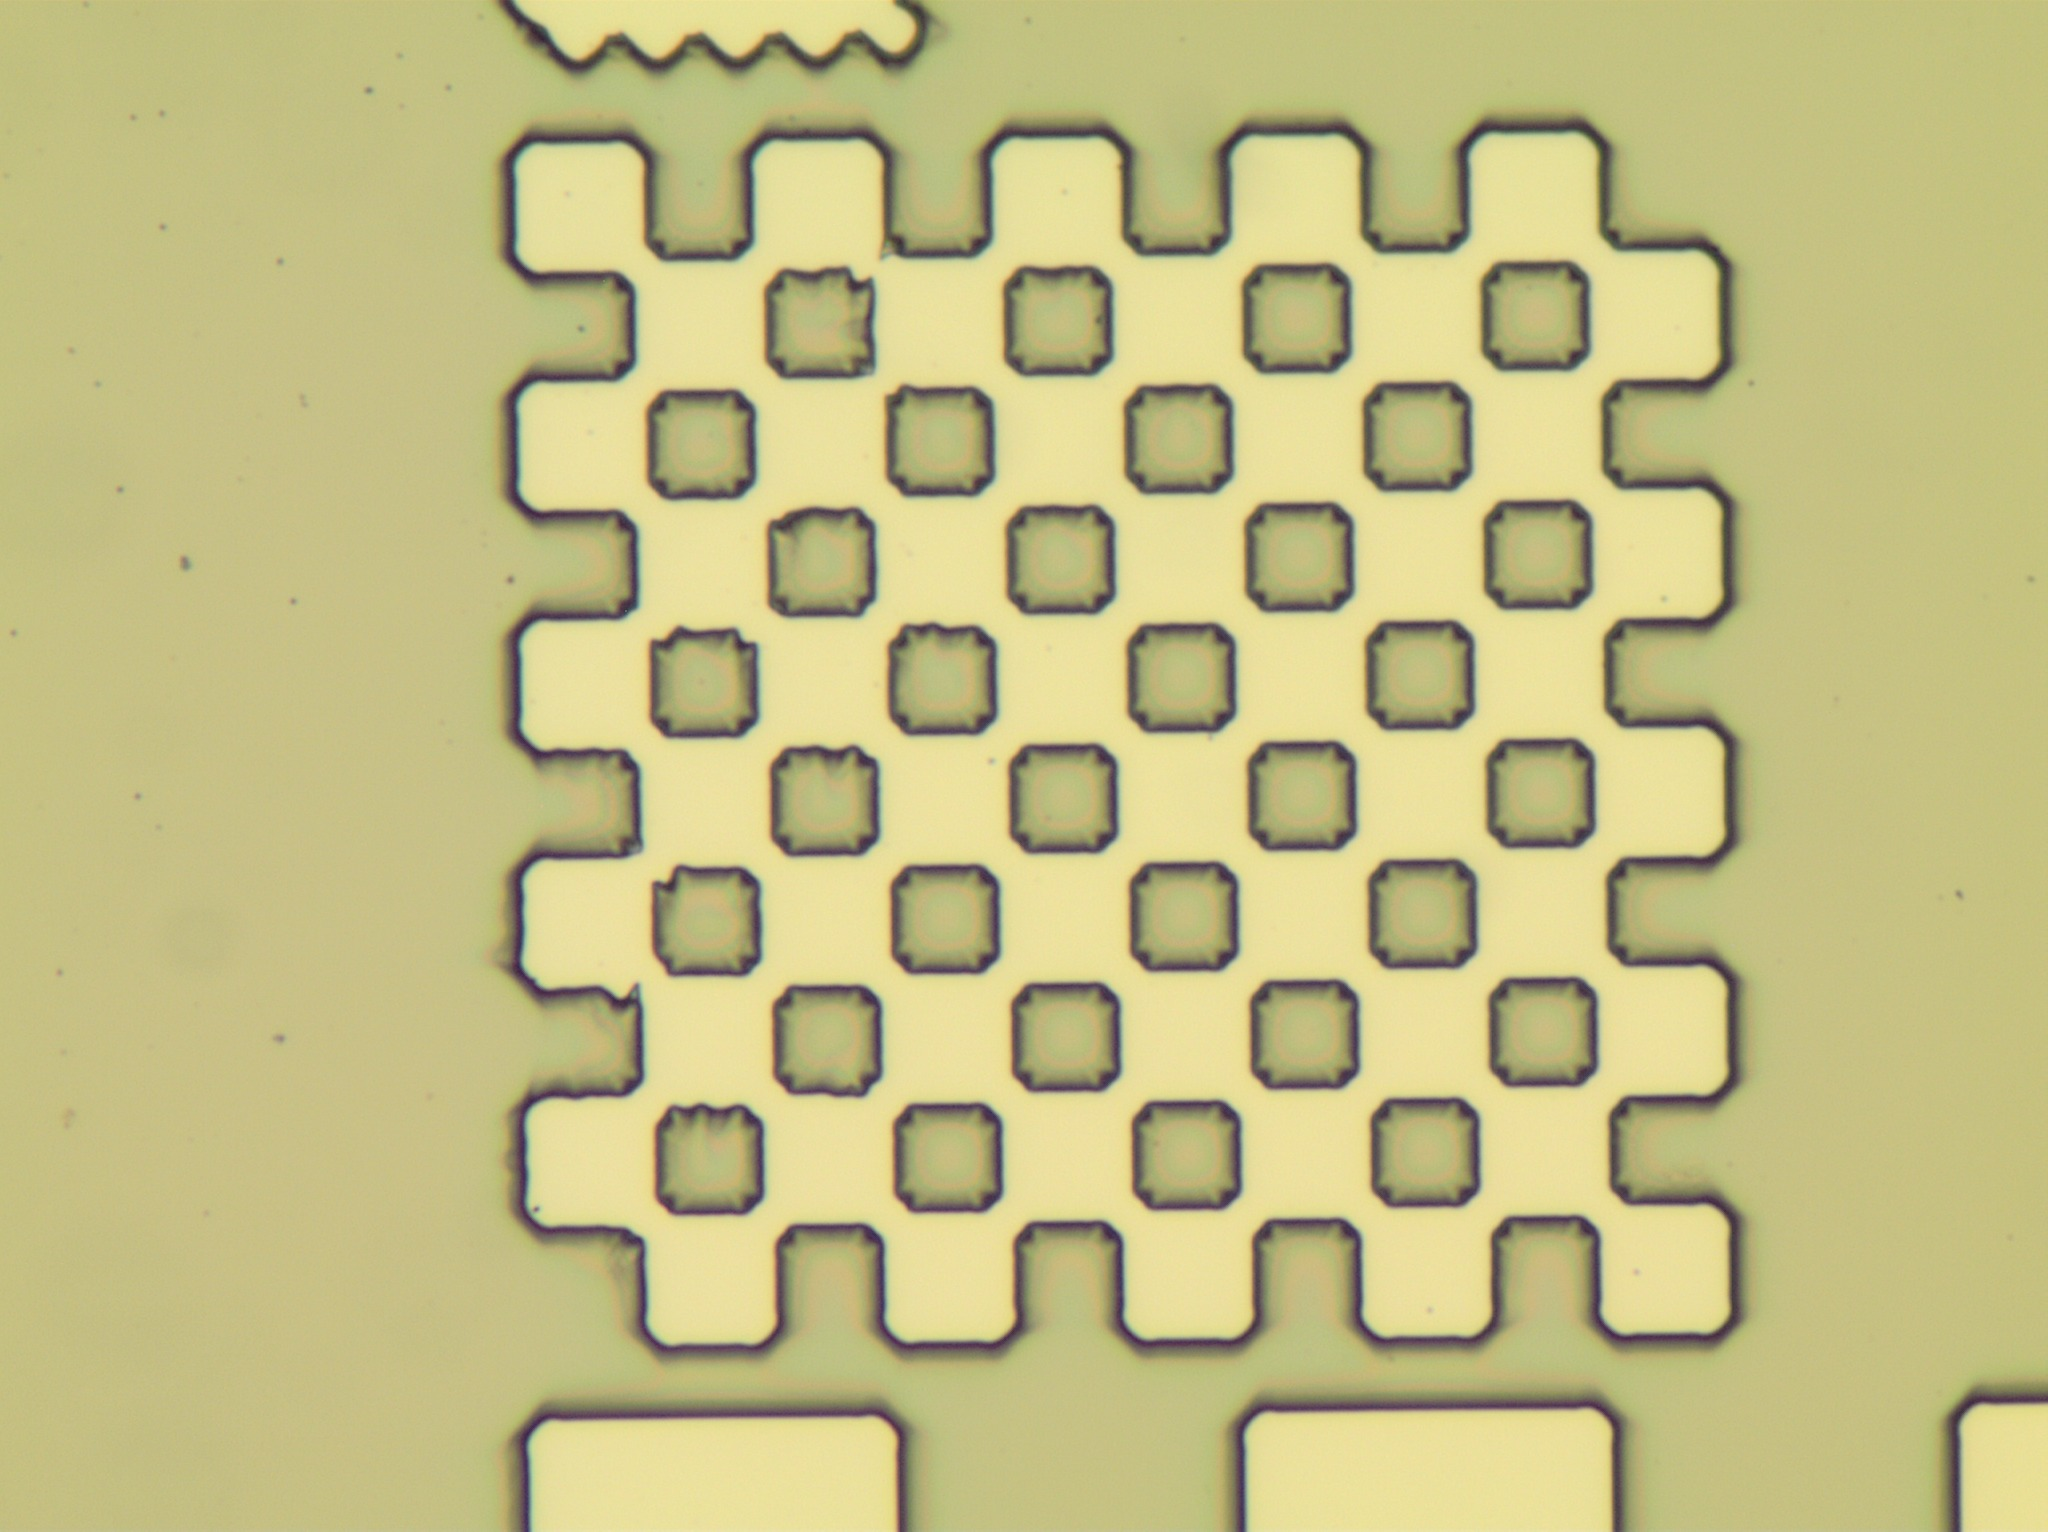
\includegraphics{data/b3f1.jpg}}
  	    \caption{Exposure time of 4.0 minutes}
  	    \label{fig:b3f1}
    \end{subfigure}
    \caption{Optical microscope images of the positive tone samples for several exposure times. Images were taken in reflection mode.}
\end{figure*}



% % \todo[inline]{Optical microscope images of samples}
% \begin{figure*}[!t]
%     \centering
%     \begin{subfigure}[t]{0.32\linewidth}
%  	\resizebox{\linewidth}{!}{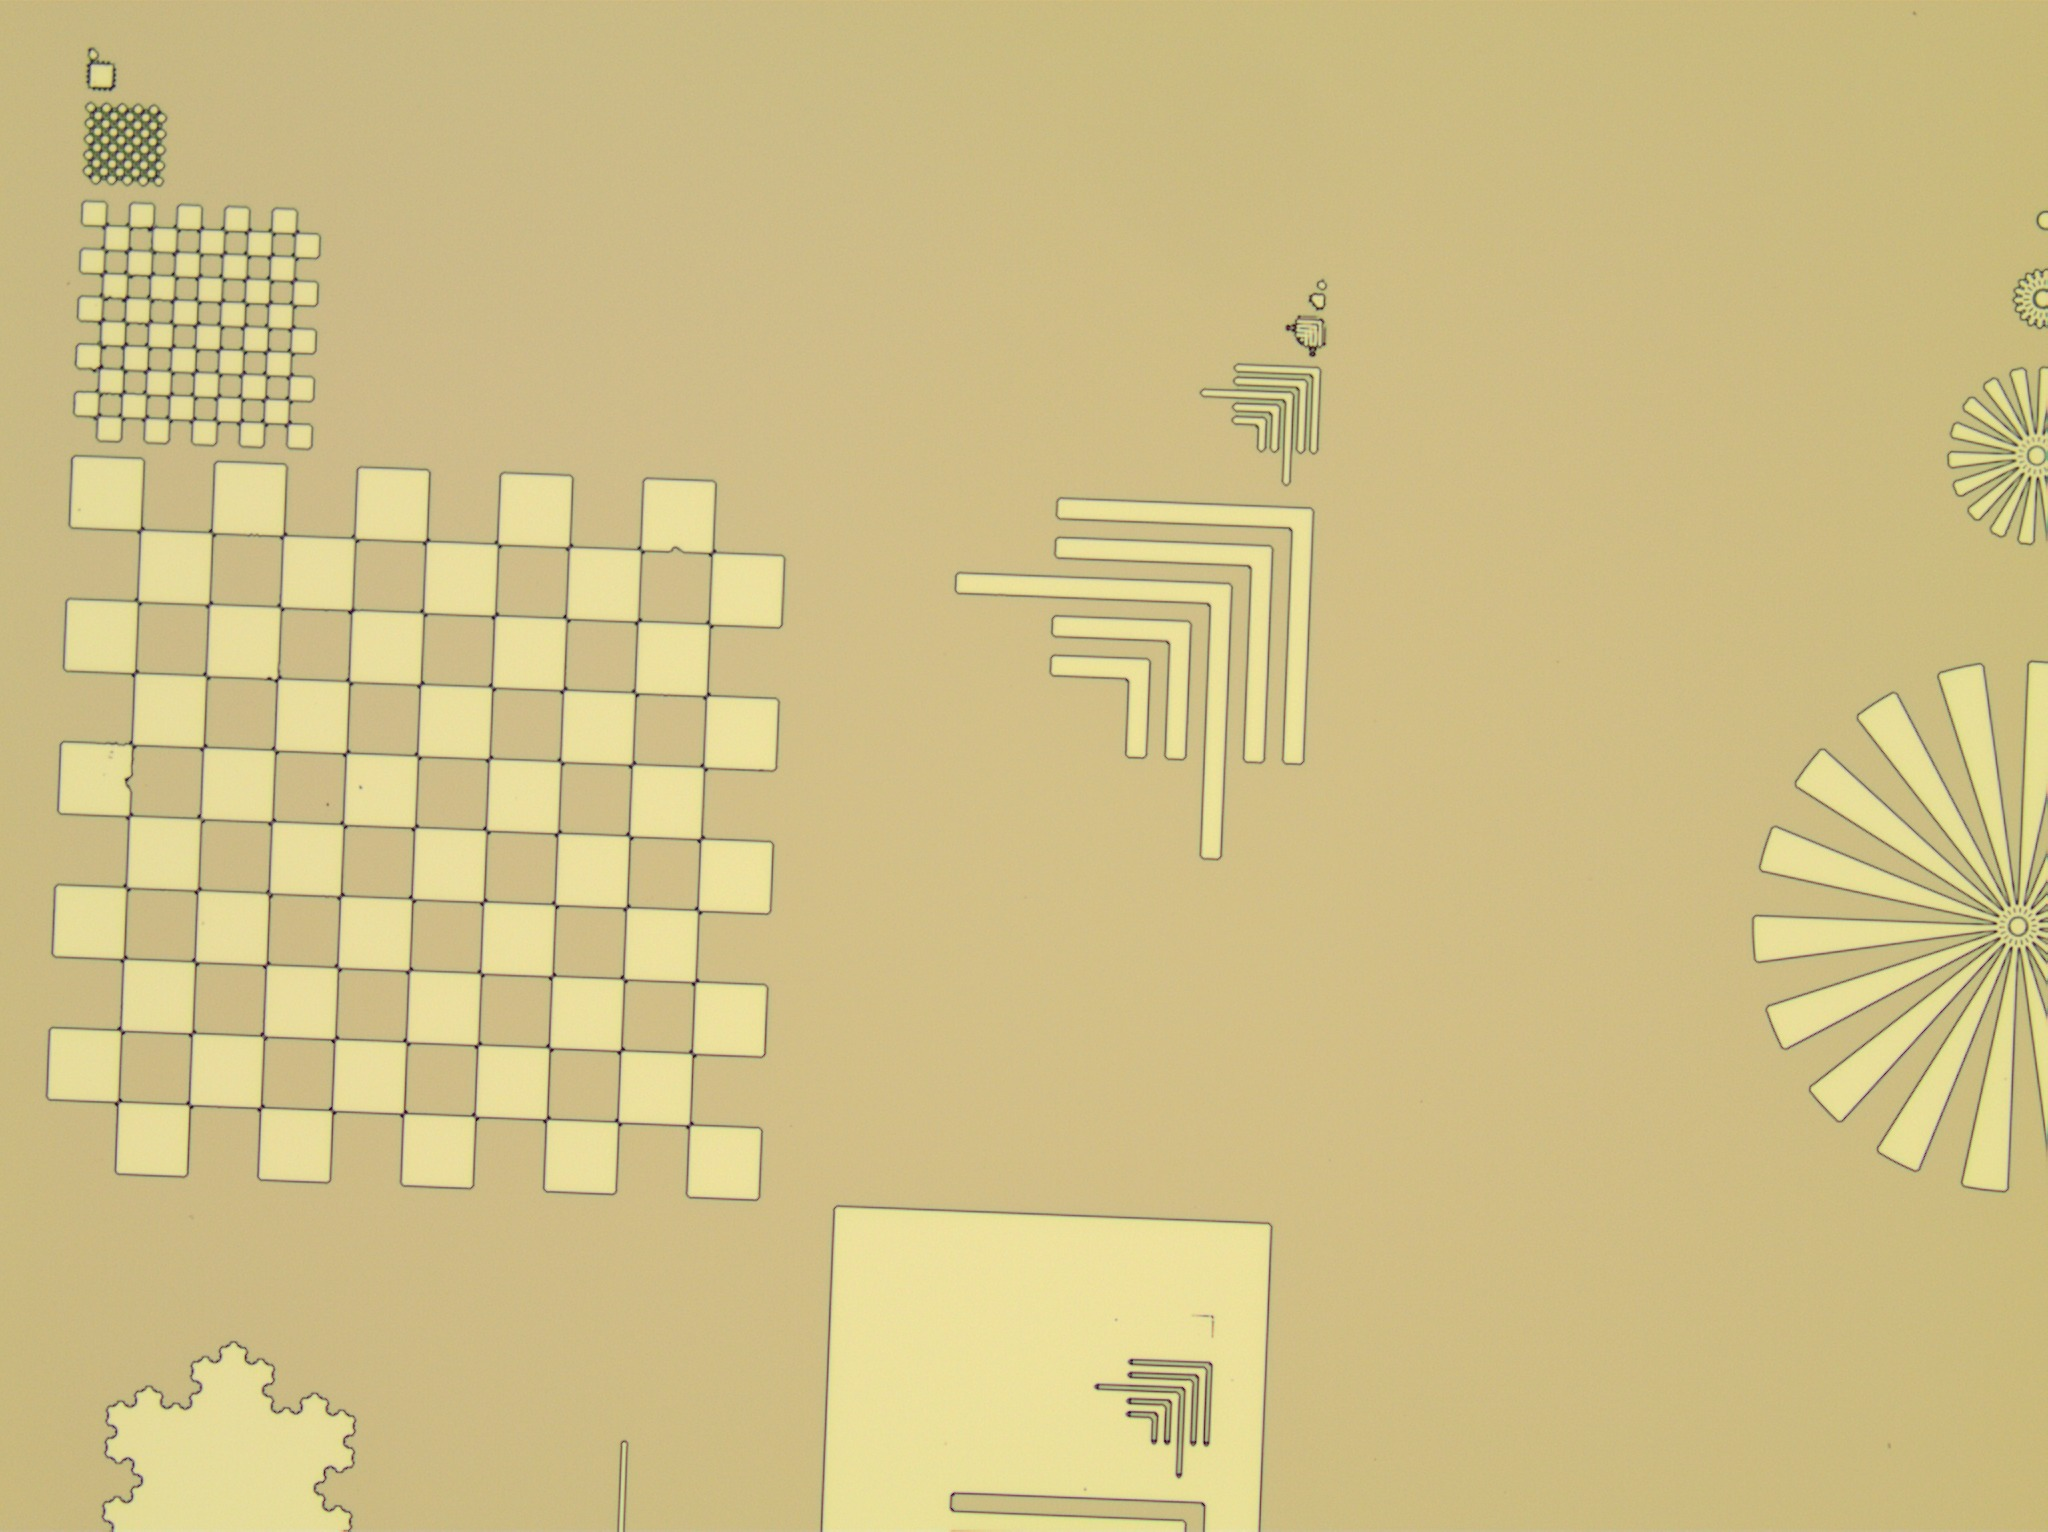
\includegraphics{data/b3b1.jpg}}
%  	\caption{b3b1}
%  	\label{fig:b3b1}
%  \end{subfigure}
% \hfill
%     \begin{subfigure}[t]{0.32\linewidth}
%  	\centering
%  	\resizebox{\linewidth}{!}{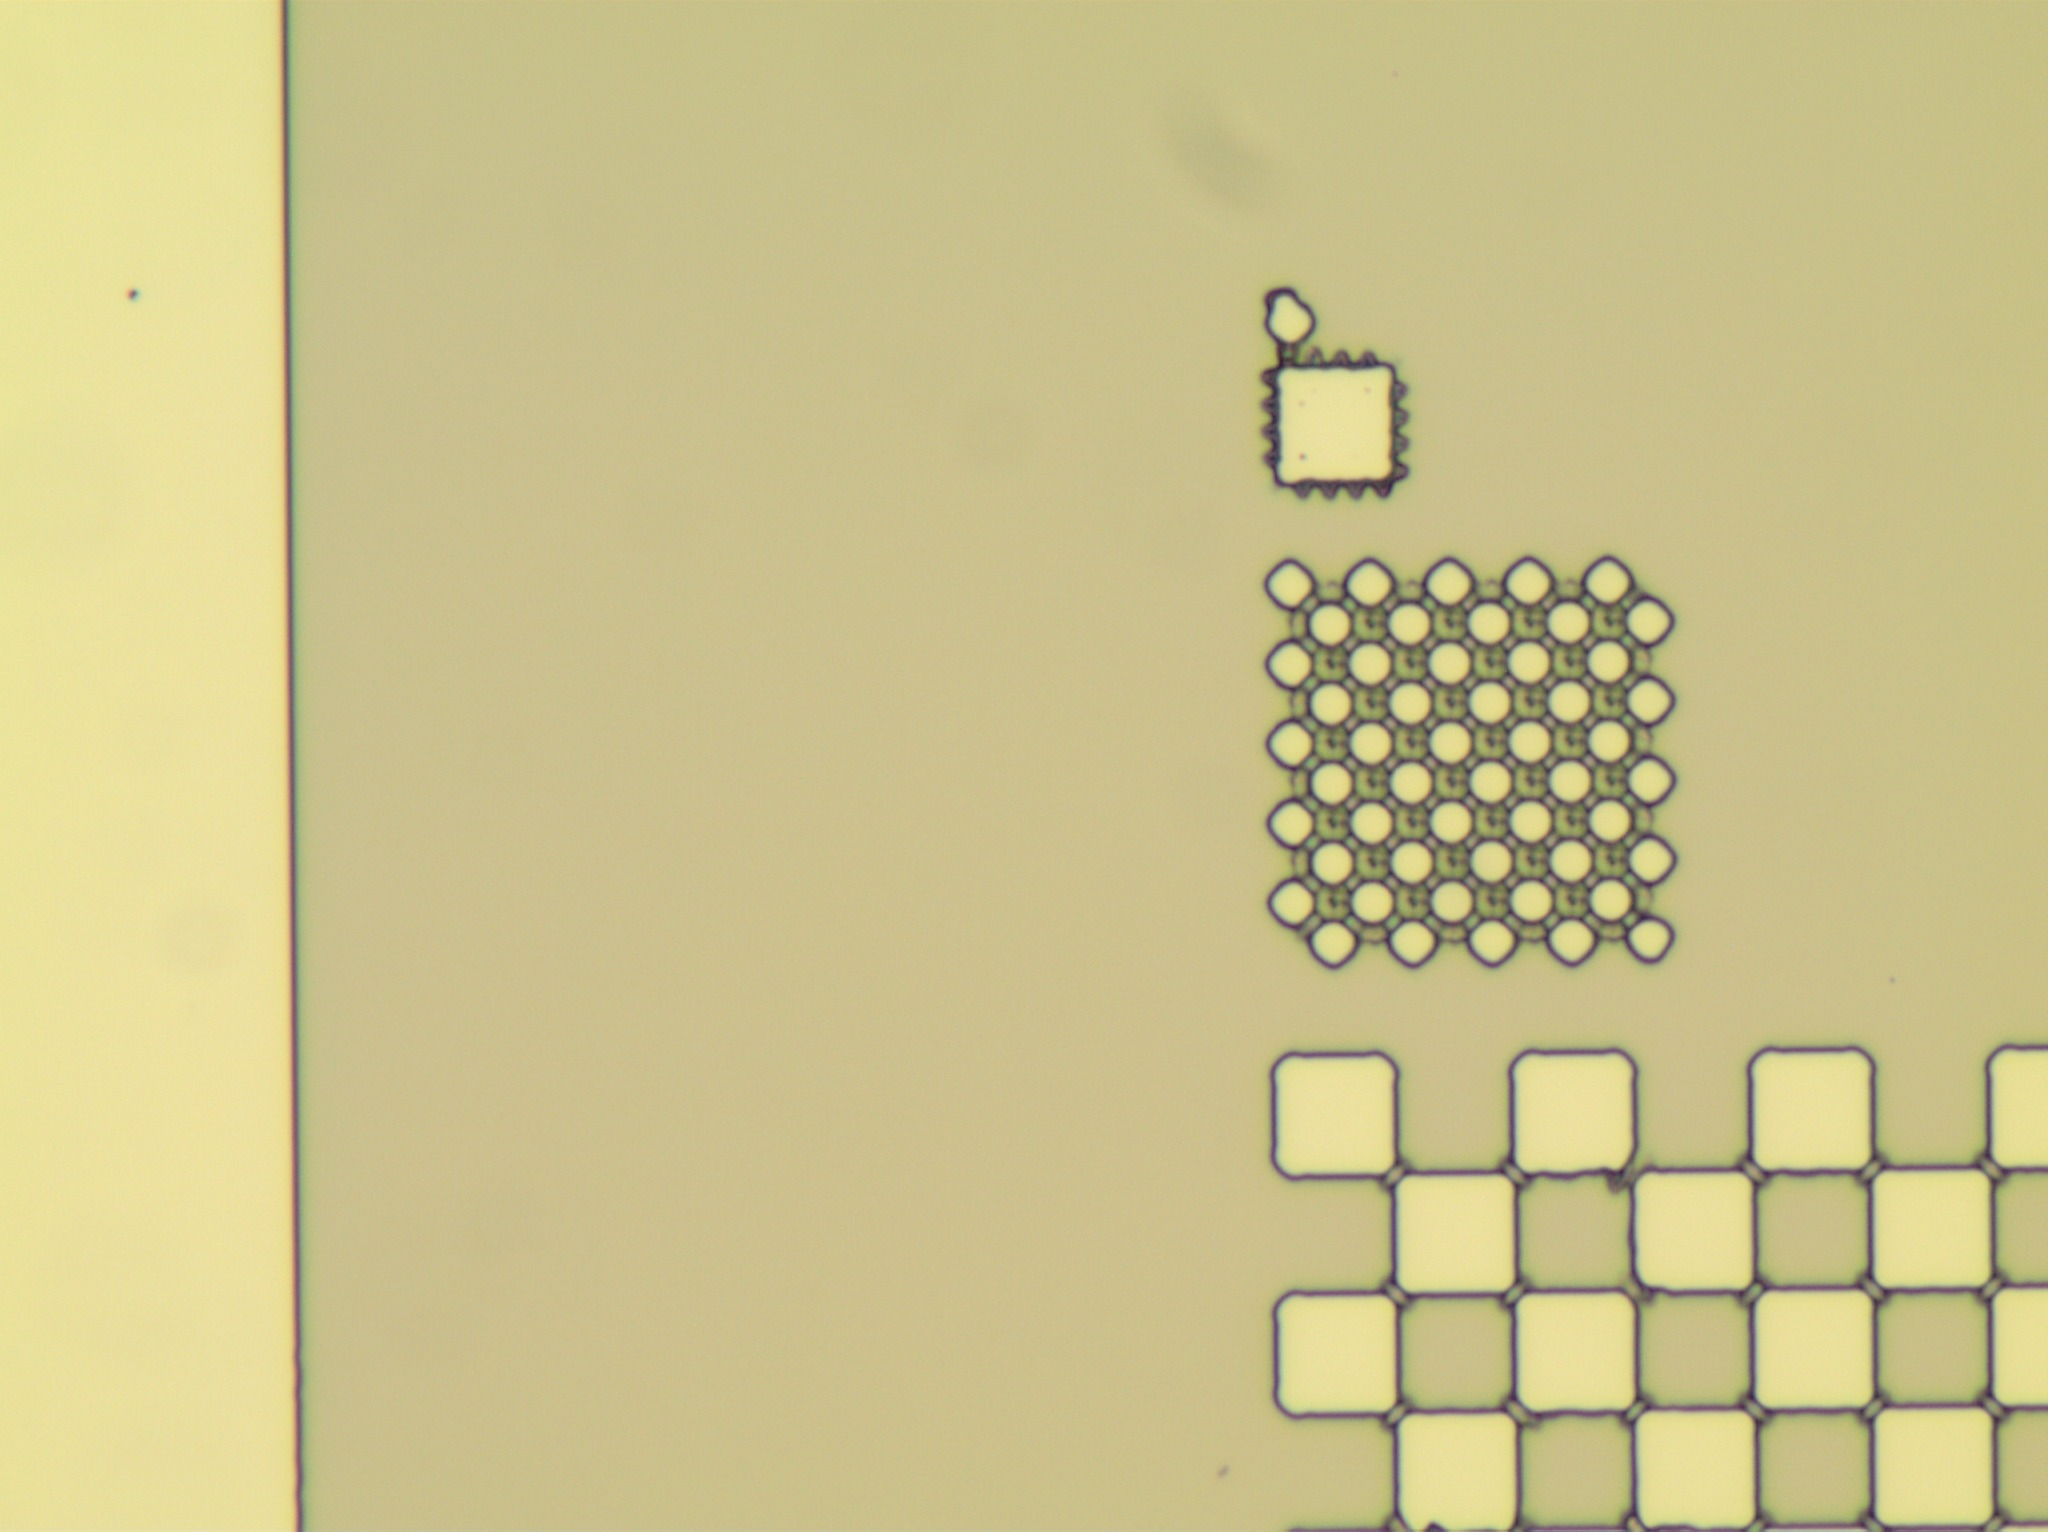
\includegraphics{data/b3b2.jpg}}
%  	\caption{b3b2}
%  	\label{fig:b3b2}
%  \end{subfigure}
% \hfill
%     \begin{subfigure}[t]{0.32\linewidth}
%  	\centering
%  	\resizebox{\linewidth}{!}{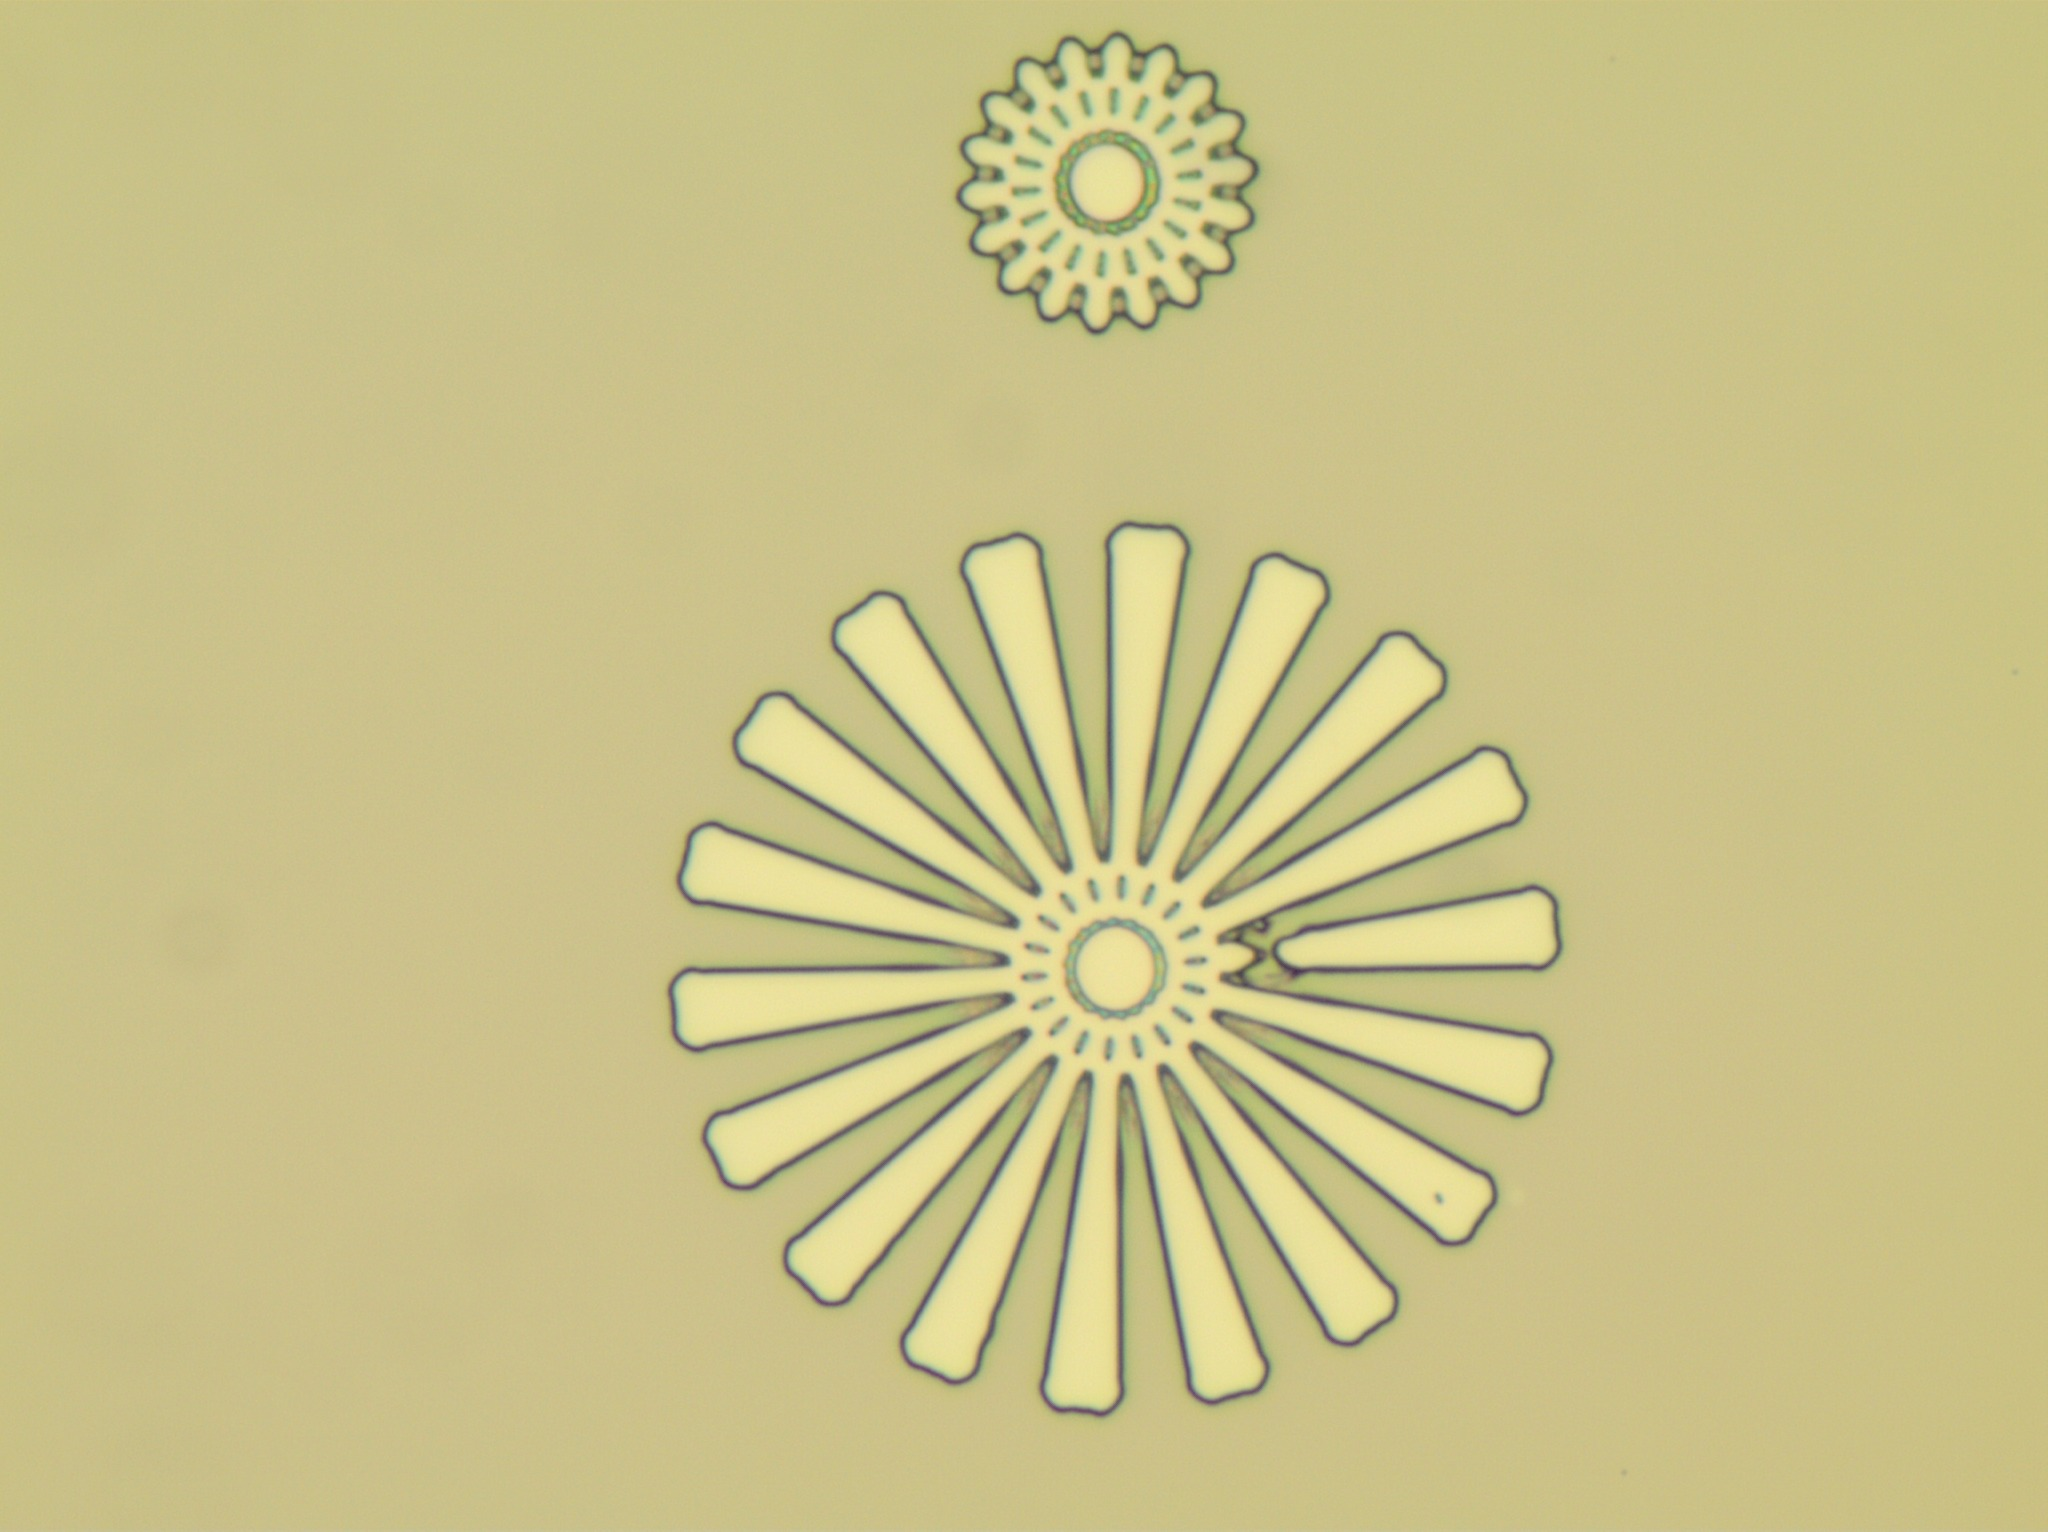
\includegraphics{data/b3b3.jpg}}
%  	\caption{b3b3}
%  	\label{fig:b3b3}
%  \end{subfigure}\\
%     \centering
%     \begin{subfigure}[t]{0.32\linewidth}
%  	\resizebox{\linewidth}{!}{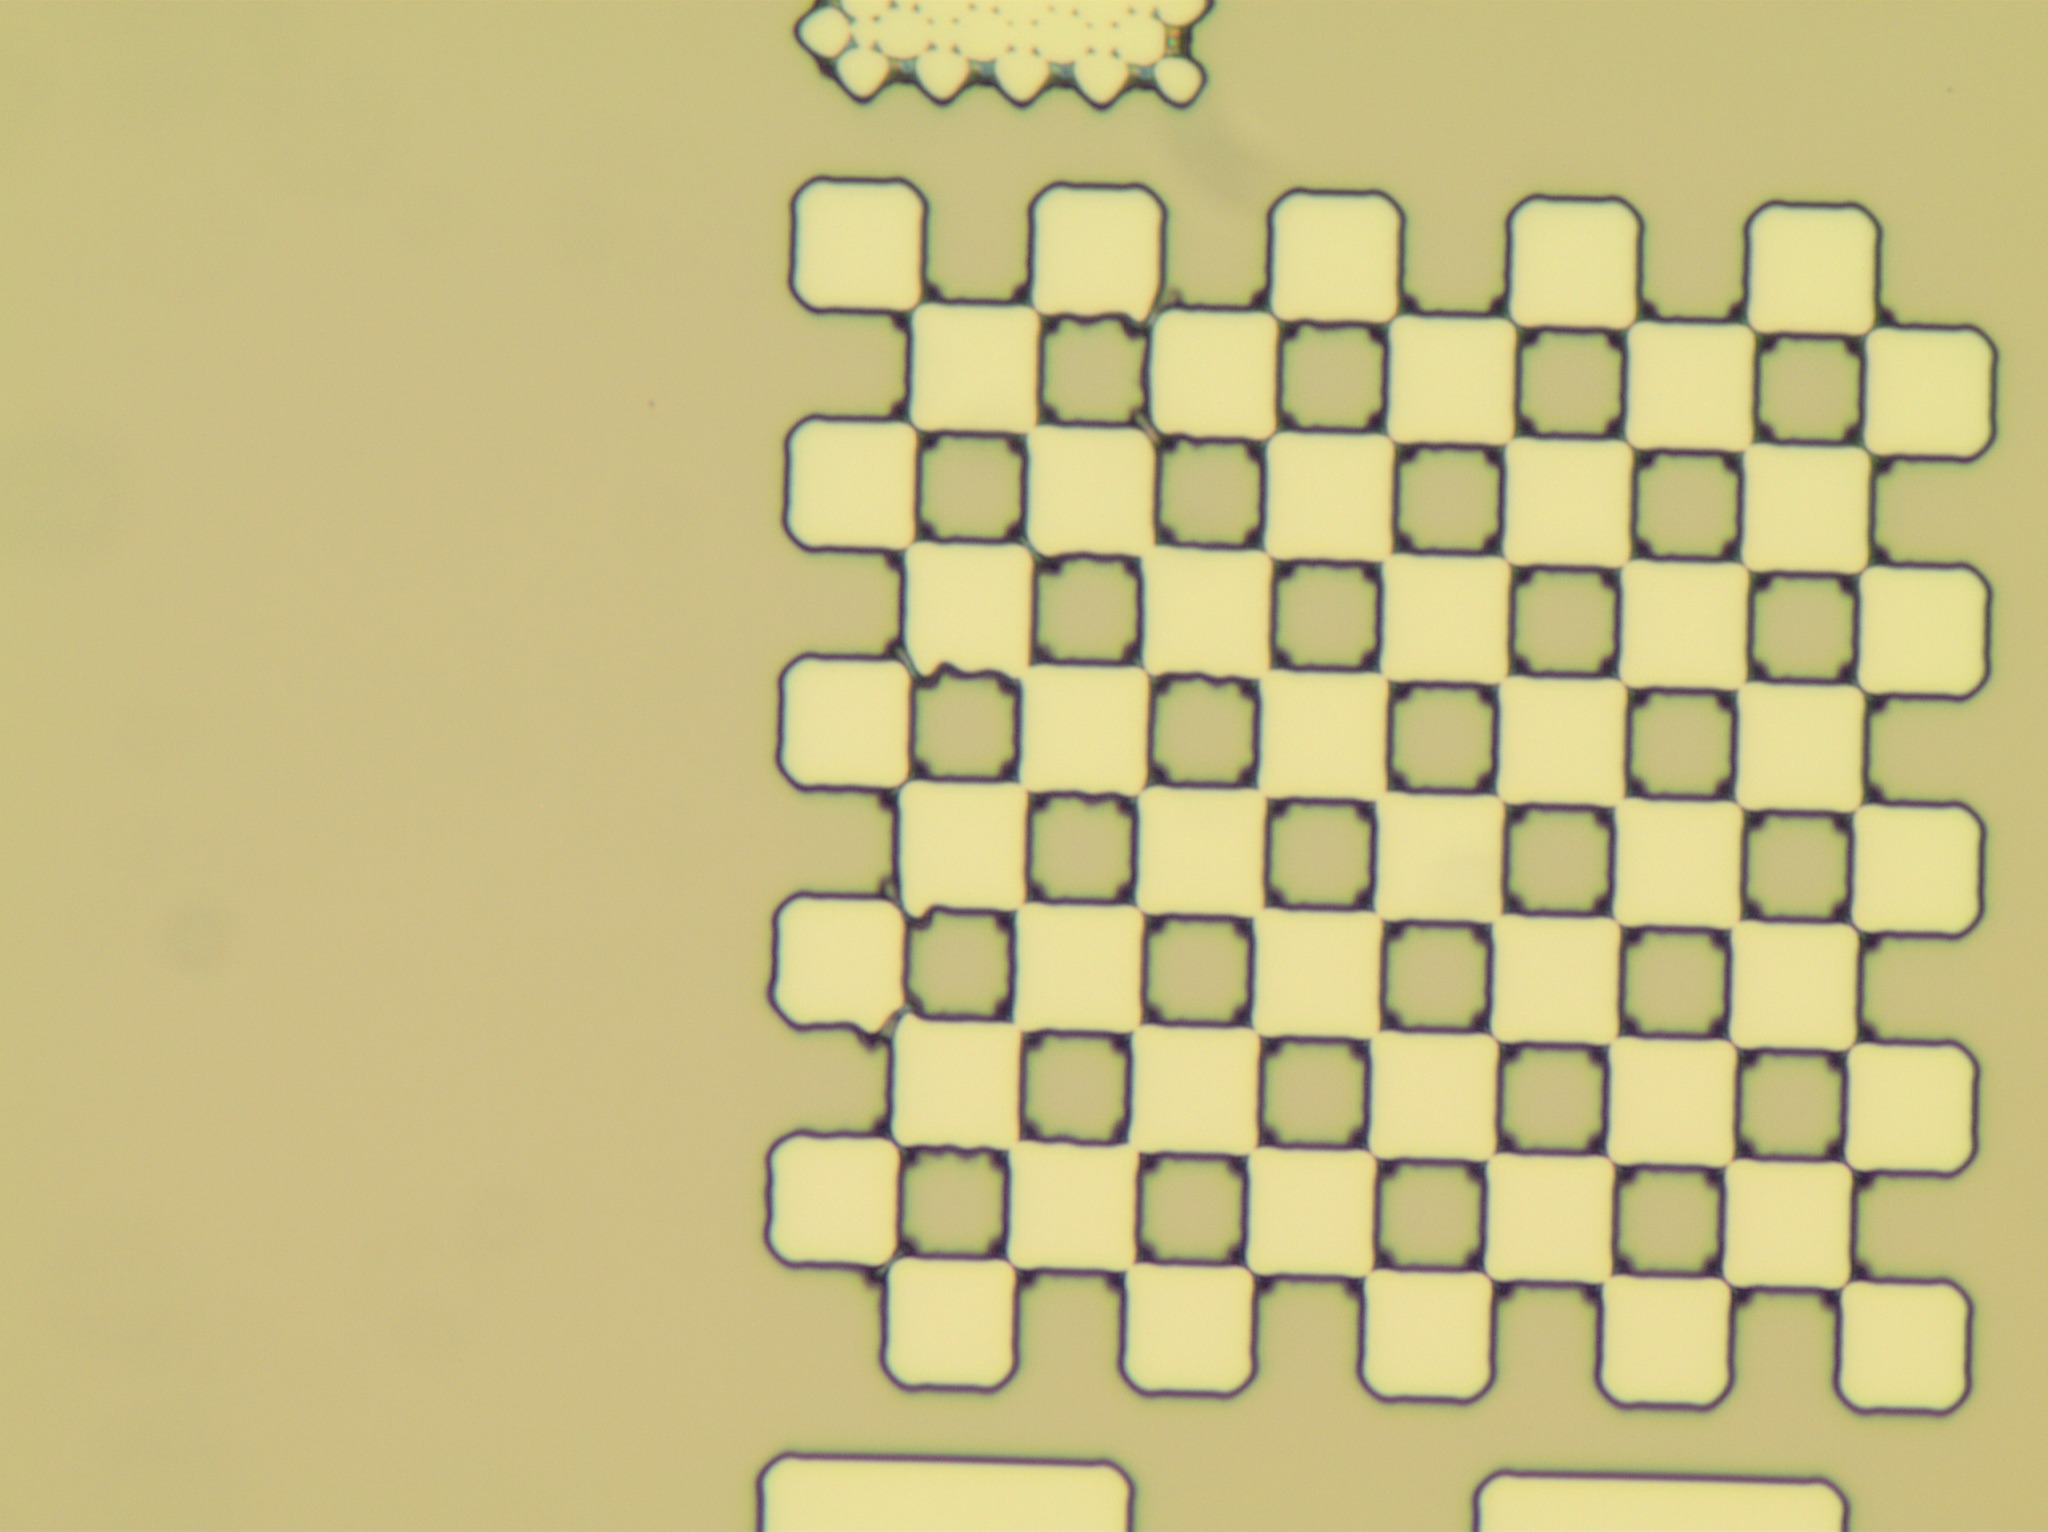
\includegraphics{data/b3c1.jpg}}
%  	\caption{b3c1}
%  	\label{fig:b3c1}
%  \end{subfigure}
% \hspace{10mm}
% \begin{subfigure}[t]{0.32\linewidth}
%  	\centering
%  	\resizebox{\linewidth}{!}{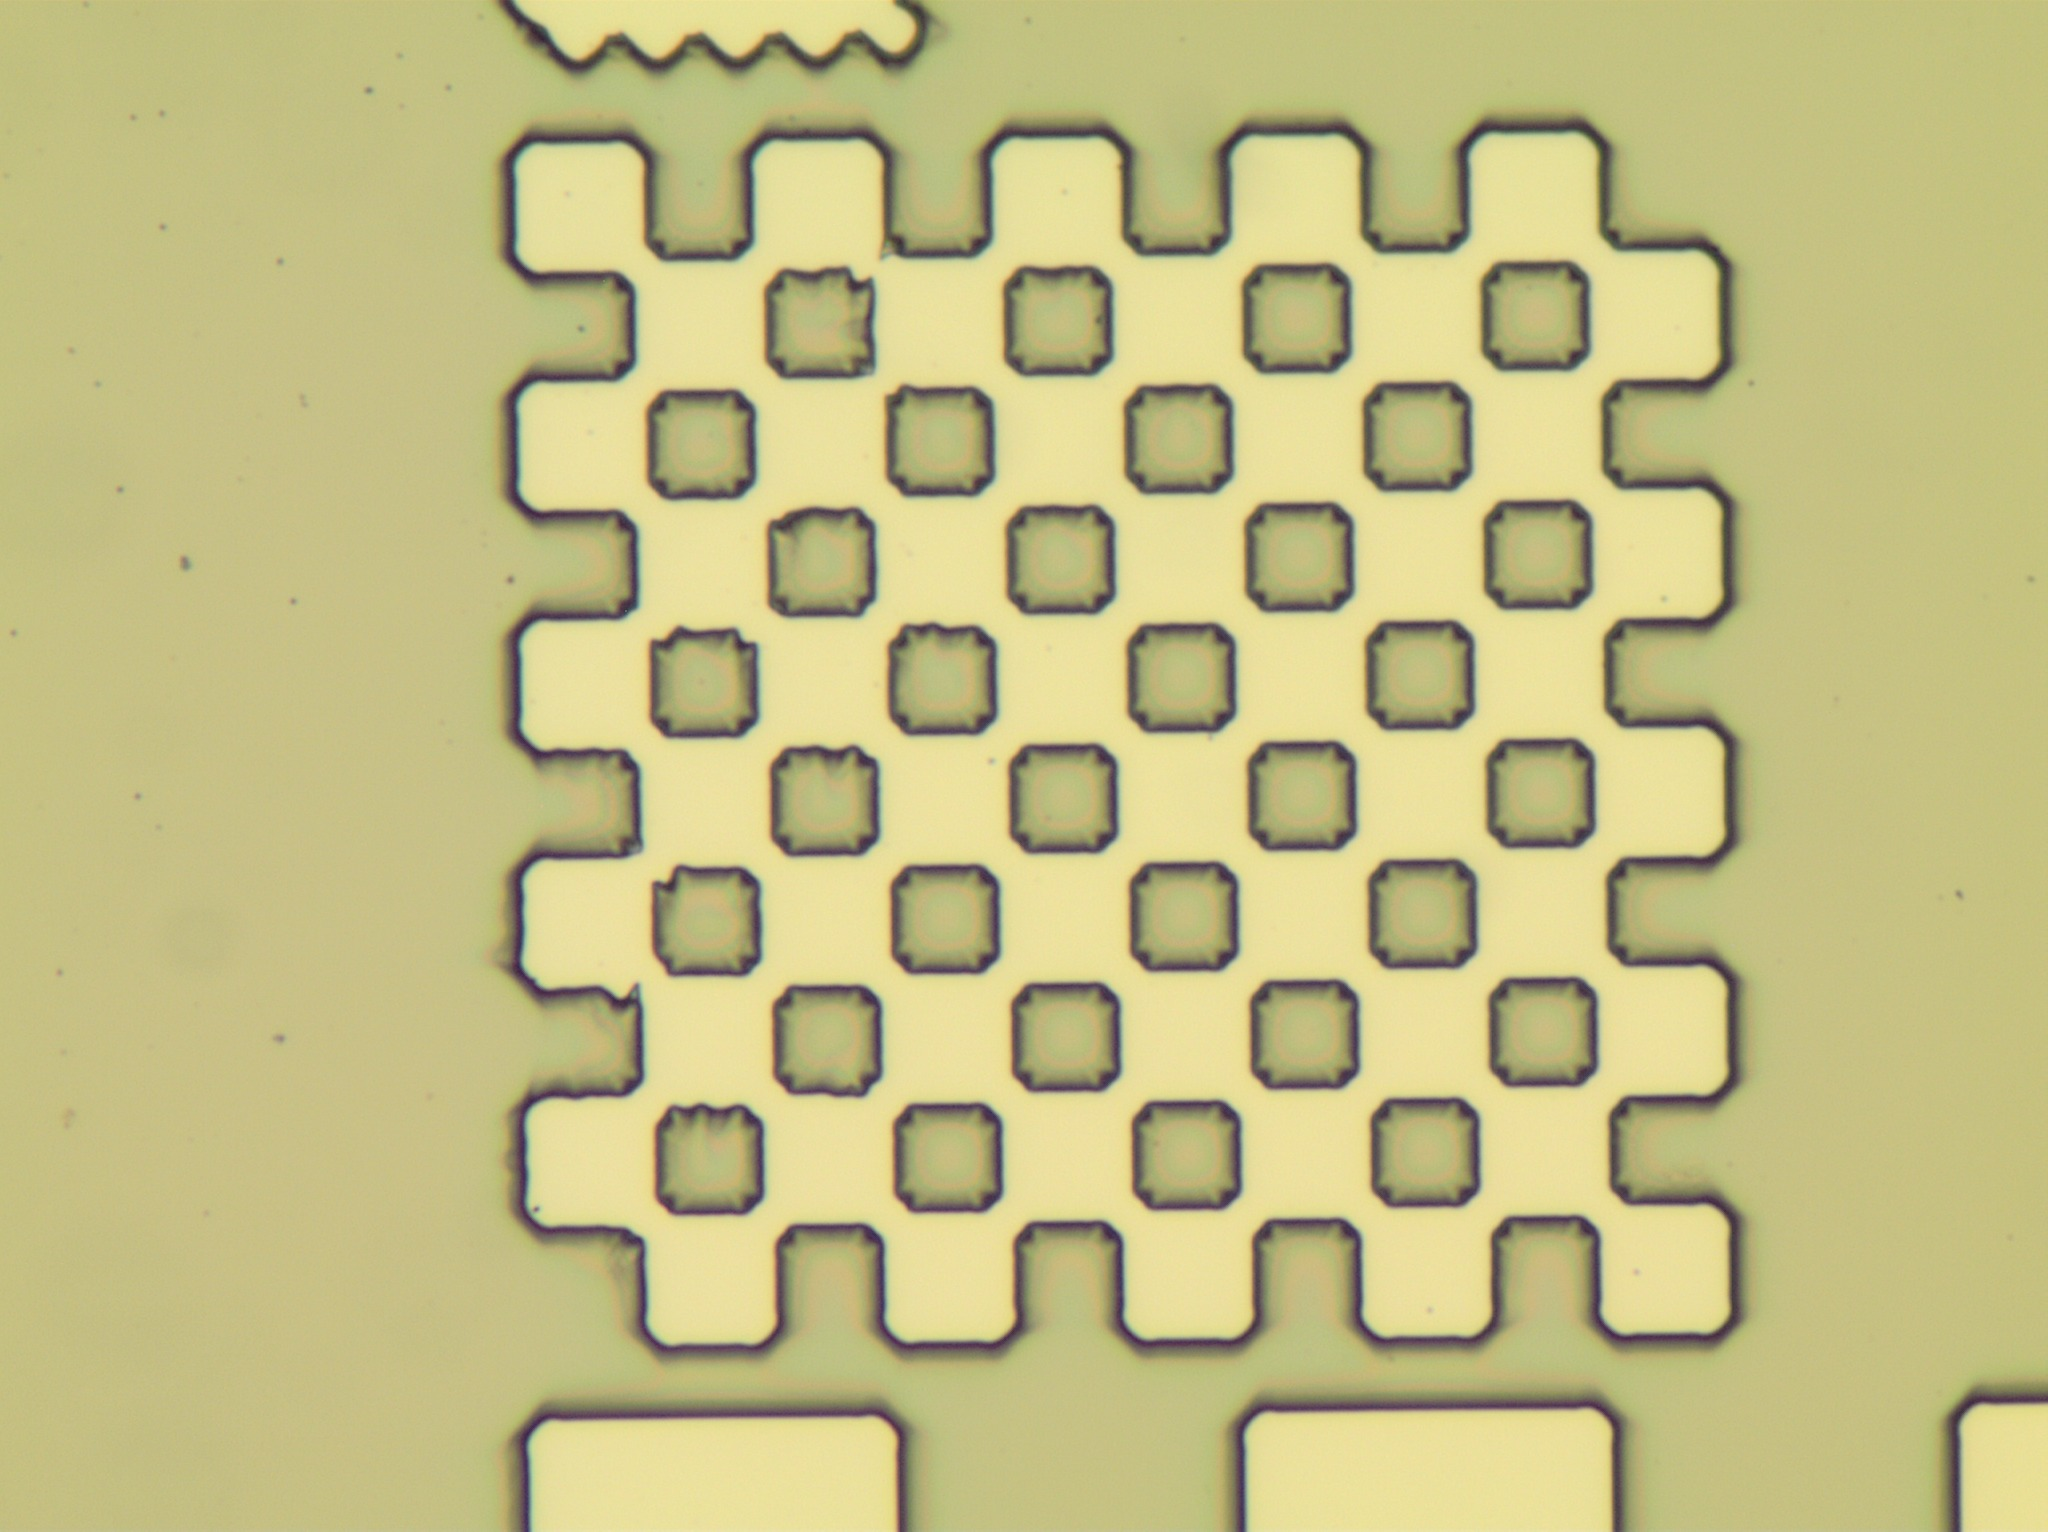
\includegraphics{data/b3f1.jpg}}
%  	\caption{b3f1}
%  	\label{fig:b3f1}
% \end{subfigure}
%  \end{figure*}
%

 % \todo[inline]{SEM}
\begin{figure*}[htb]
    \centering
    \begin{subfigure}[t]{0.32\linewidth}
  	    \resizebox{\linewidth}{!}{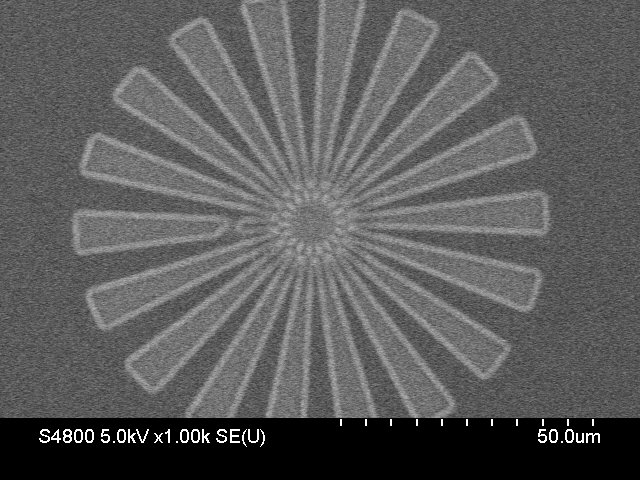
\includegraphics{data/sem/b3a1_q01.jpg}}
      	\caption{Structure size of $\sim$6 $\mu$m. There is a small defect in the line pattern on the left side, which was most likely caused by improper handling of the sample.}
      	\label{fig:b2d1_q1}
    \end{subfigure}
    \hfill
    \begin{subfigure}[t]{0.32\linewidth}
      	\resizebox{\linewidth}{!}{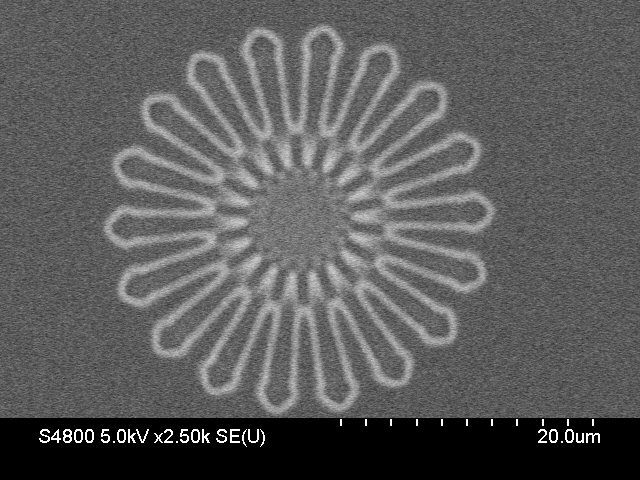
\includegraphics{data/sem/b3a2_q02.jpg}}
      	\caption{Structure size of $\sim$2 $\mu$m. The pattern loses its structure near the center due to interference effects.}
      	\label{fig:b2d2_q2}
    \end{subfigure}
    \hfill
    \begin{subfigure}[t]{0.32\linewidth}
      	\resizebox{\linewidth}{!}{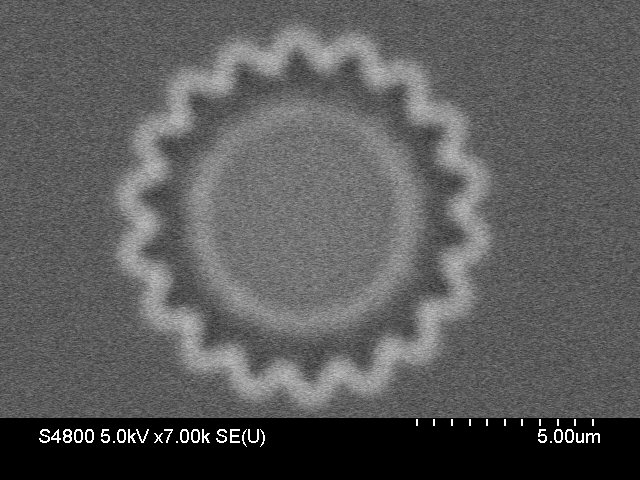
\includegraphics{data/sem/b3a3_q03.jpg}}
      	\caption{Structure size of $\sim$1 $\mu$m. Almost the whole pattern is dominated by interference at these length scales.}
      	\label{fig:b2d3_q3}
    \end{subfigure}
    \caption{SEM images of outward radiating lines pattern on the positive tone sample with $\tau = 2$ min. For the structure size the width of the line at the edge of the pattern is taken as guideline.}
\end{figure*}

\begin{figure*}[!t]
    \centering
    \begin{subfigure}[t]{0.24\linewidth}
      	\resizebox{\linewidth}{!}{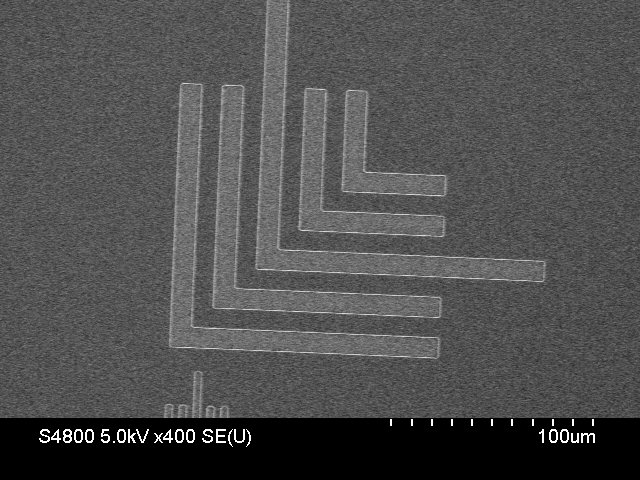
\includegraphics{data/sem/b3a11_q12.jpg}}
      	\caption{Structure size of $\sim$12 $\mu$m.}
      	\label{fig:b2d12_q12}
    \end{subfigure}
    \hfill
    \begin{subfigure}[t]{0.24\linewidth}
      	\resizebox{\linewidth}{!}{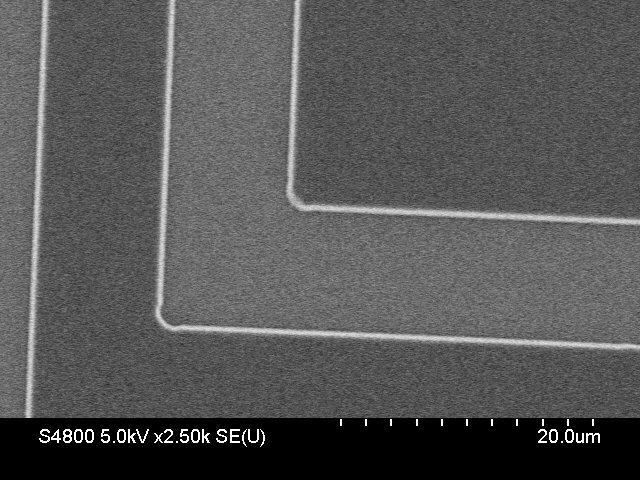
\includegraphics{data/sem/b3a11_q13.jpg}}
      	\caption{Zoom of the previous picture. Rounding off the corners can be seen. These could in principle be corrected by using OPC.}
      	\label{fig:b2d13_q13}
    \end{subfigure}
 %\hfill
 %    \begin{subfigure}[t]{0.24\linewidth}
 % 	\centering
 % 	\resizebox{\linewidth}{!}{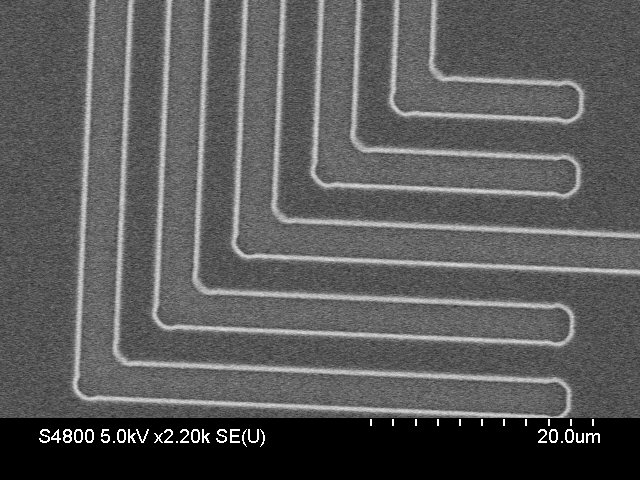
\includegraphics{data/sem/b3a11_q14.jpg}}
 % 	\caption{SEM}
 % 	\label{fig:b2d14_q14}
 %  \end{subfigure}
    \hfill
    \begin{subfigure}[t]{0.24\linewidth}
      	\resizebox{\linewidth}{!}{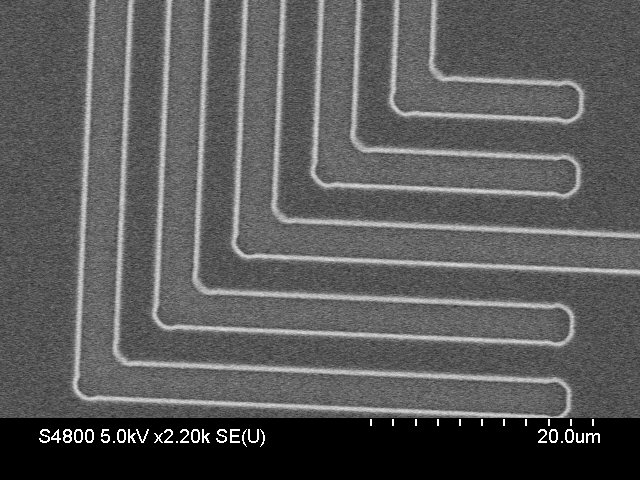
\includegraphics{data/sem/b3a11_q15.jpg}}
      	\caption{Structure size of $\sim$1.5 $\mu$m. The rounding of the corners has become more pronounced.}
      	\label{fig:b2d15_q15}
    \end{subfigure}
    \hfill
    \begin{subfigure}[t]{0.24\linewidth}
      	\resizebox{\linewidth}{!}{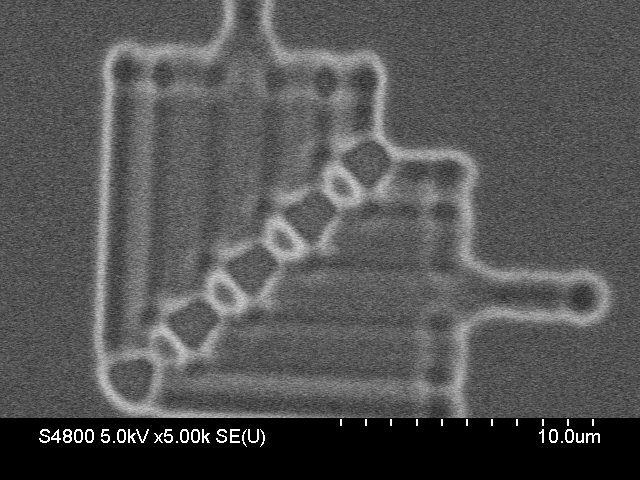
\includegraphics{data/sem/b3a11_q16.jpg}}
      	\caption{Severe interference effects start to occur at the bends for structure sizes $\sim$1$\mu$m.}
      	\label{fig:b2d16_q16}
    \end{subfigure}
    \caption{SEM images of a single line surrounded by multiple lines on the positive tone sample with $\tau = 2$ min. For the structure size the width of the line is taken as guideline.}
\end{figure*}

 \begin{figure*}[htb]
     \centering
%     \begin{subfigure}[t]{0.24\linewidth}
%  	\centering
%  	\resizebox{\linewidth}{!}{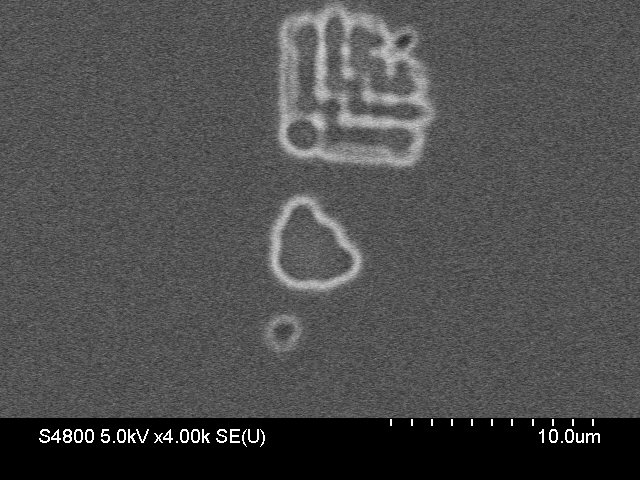
\includegraphics{data/sem/b3a11_q17.jpg}}
%  	\caption{SEM}
%  	\label{fig:b2d17_q17}
%  \end{subfigure}
% \hfill
 %    \begin{subfigure}[t]{0.24\linewidth}
 % 	\centering
 % 	\resizebox{\linewidth}{!}{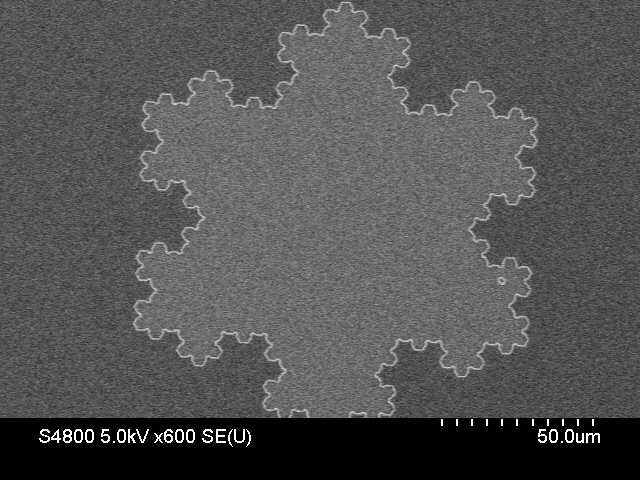
\includegraphics{data/sem/b3a11_q18.jpg}}
 % 	\caption{SEM}
 % 	\label{fig:b2d18_q18}
 % \end{subfigure}
 %\hfill
    \begin{subfigure}[t]{0.32\linewidth}
      	\resizebox{\linewidth}{!}{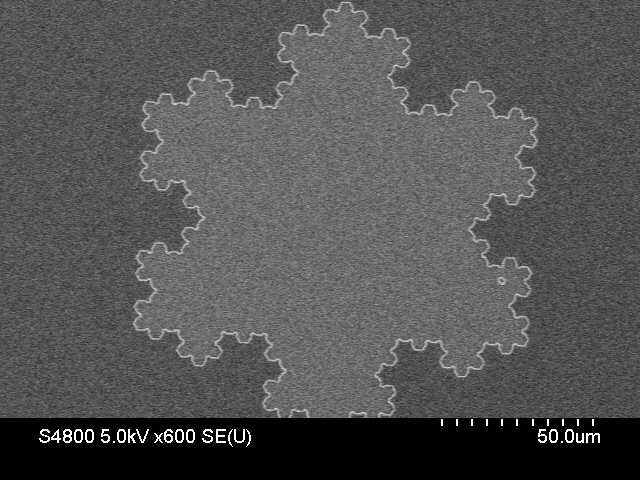
\includegraphics{data/sem/b3a11_q19.jpg}}
      	\caption{Structure size of $\sim$50 $\mu$m.}
      	\label{fig:b2d19_q19}
    \end{subfigure}
    \hfill
    \begin{subfigure}[t]{0.32\linewidth}
      	\resizebox{\linewidth}{!}{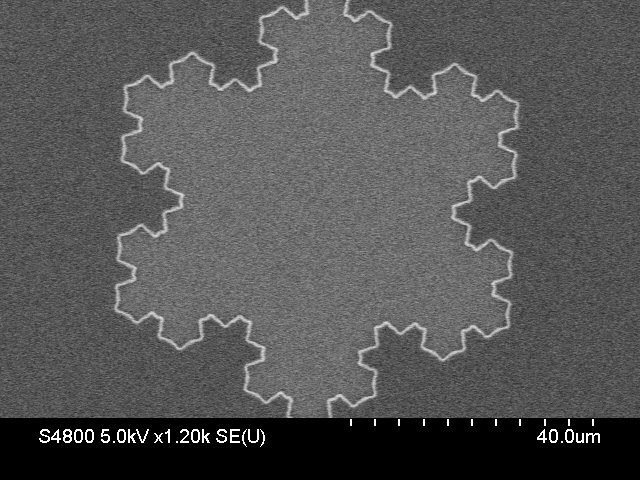
\includegraphics{data/sem/b3a11_q20.jpg}}
      	\caption{Structure size of $\sim$30 $\mu$m. In comparison with the previous image, a significant drop in detail can be seen at the eges.}
      	\label{fig:b2d20_q20}
    \end{subfigure}
    \hfill
    \begin{subfigure}[t]{0.32\linewidth}
      	\resizebox{\linewidth}{!}{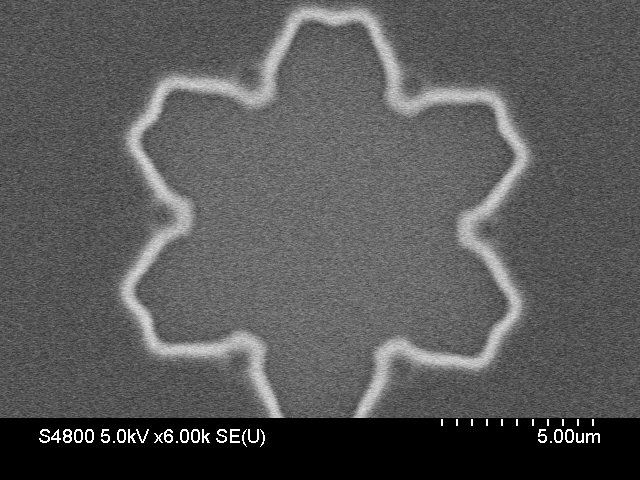
\includegraphics{data/sem/b3a11_q21.jpg}}
      	\caption{Structure size of $\sim$4 $\mu$m. All fine details have been lost.}
      	\label{fig:b2d21_q21}
    \end{subfigure}
    \caption{SEM images of Koch snowflake on the positive tone $\tau = 2$ min. For the structure size the width of one of the bulbs is taken as guideline.}
\end{figure*}

\begin{figure*}[htb]
    \centering
    \begin{subfigure}[t]{0.24\linewidth}
      	\resizebox{\linewidth}{!}{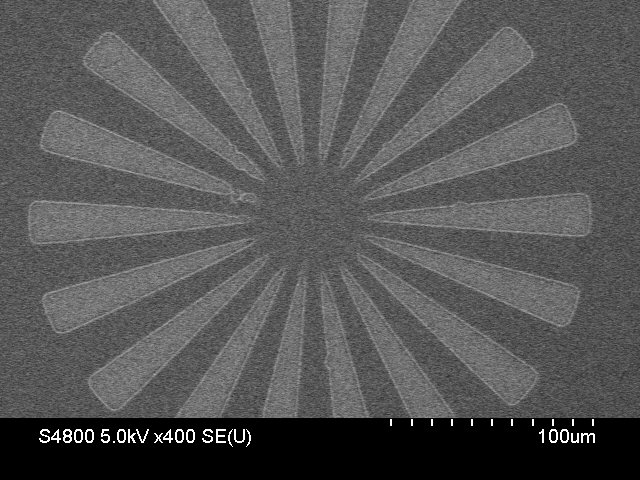
\includegraphics{data/sem/b2d22_q22.jpg}}
      	\caption{Structure size of $\sim$20 $\mu$m. Already at these length scales rounding of the corners can be seen. The pattern disappears in the center due to the overexposure.}
      	\label{fig:b2d22_q22}
    \end{subfigure}
    \hfill
    \begin{subfigure}[t]{0.24\linewidth}
      	\resizebox{\linewidth}{!}{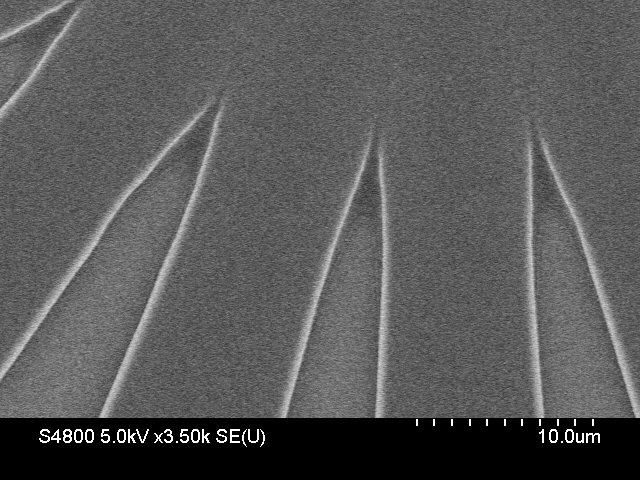
\includegraphics{data/sem/b2d23_q23.jpg}}
      	\caption{Zoom in of the previous picture, to display how the pattern tapers of due to overexposure.}
      	\label{fig:b2d23_q23}
    \end{subfigure}
    \hfill
    \begin{subfigure}[t]{0.24\linewidth}
      	\resizebox{\linewidth}{!}{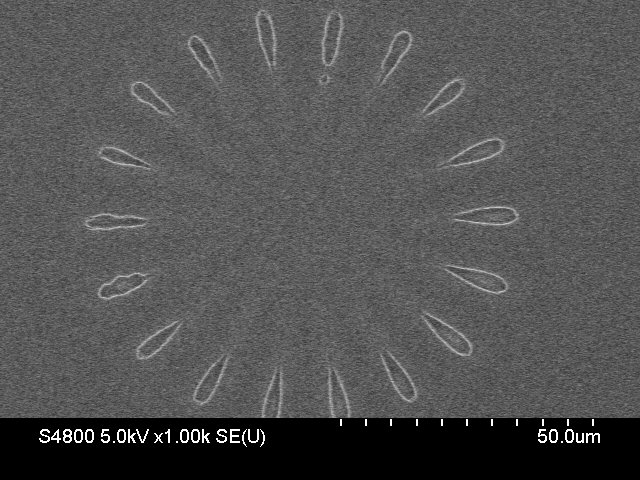
\includegraphics{data/sem/b2d24_q24.jpg}}
      	\caption{Structure size of $\sim$5 $\mu$m. The pattern is almost completely gone. Even after the tapering of the pattern, the photoactivation of the resist is still visible.}
      	\label{fig:b2d24_q24}
    \end{subfigure}
    \hfill
    \begin{subfigure}[t]{0.24\linewidth}
      	\resizebox{\linewidth}{!}{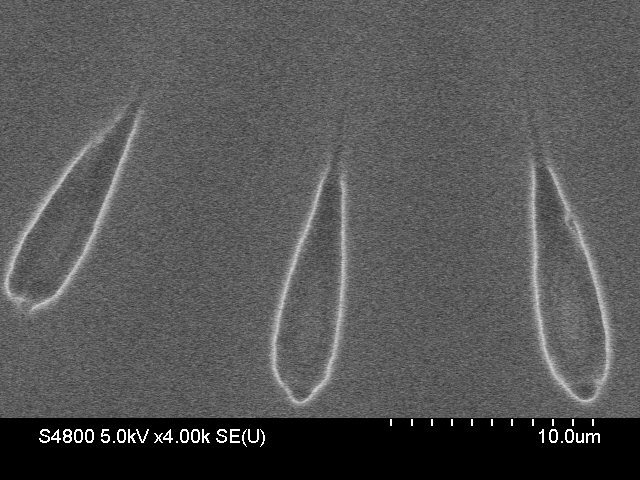
\includegraphics{data/sem/b2d25_q25.jpg}}
      	\caption{Zoom in on the previous picture.}
      	\label{fig:b2d25_q25}
    \end{subfigure}
    \hfill
    \caption{SEM images of outward radiating lines pattern on the negative tone sample with $\tau_1 = 0.5$~min. For the structure size the width of the line at the edge of the pattern is taken as guideline.}
\end{figure*}

\begin{figure*}[htb]
    \centering
    \begin{subfigure}[t]{0.24\linewidth}
  		\resizebox{\linewidth}{!}{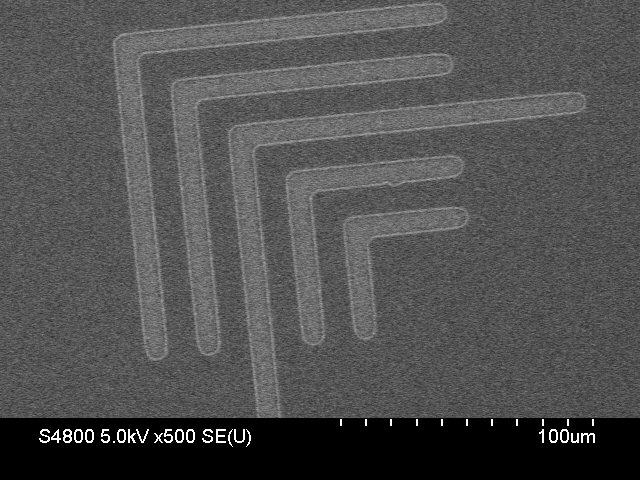
\includegraphics{data/sem/b2d30_q30.jpg}}
  	    \caption{Structure size of $\sim$10 $\mu$m.}
  	    \label{fig:b2d30_q30}
    \end{subfigure}
    \hfill
    \begin{subfigure}[t]{0.24\linewidth}
      	\resizebox{\linewidth}{!}{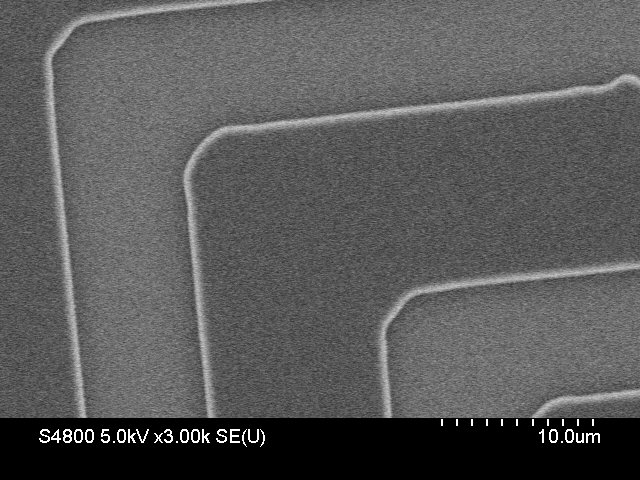
\includegraphics{data/sem/b2d31_q31.jpg}}
      	\caption{Zoom in of the previous image. Rounding of the corners can be seen.}
      	\label{fig:b2d31_q31}
    \end{subfigure}
    \hfill
    \begin{subfigure}[t]{0.24\linewidth}
  	    \resizebox{\linewidth}{!}{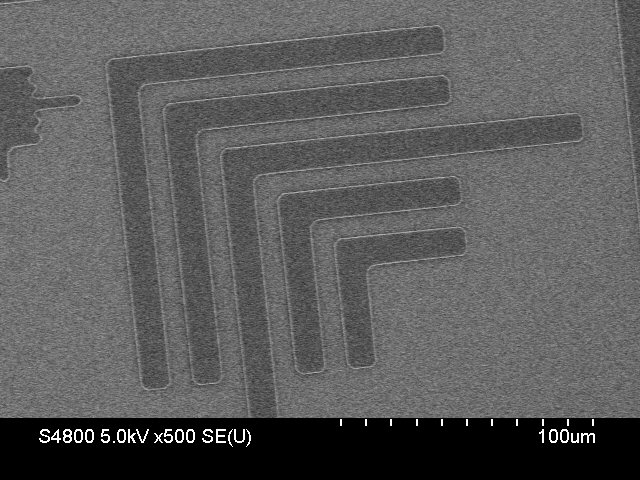
\includegraphics{data/sem/b2d31_q32.jpg}}
      	\caption{Inverse of the two previous images.}
      	\label{fig:b2d31_q32}
    \end{subfigure}
    \hfill
    \begin{subfigure}[t]{0.24\linewidth}
  	 	\resizebox{\linewidth}{!}{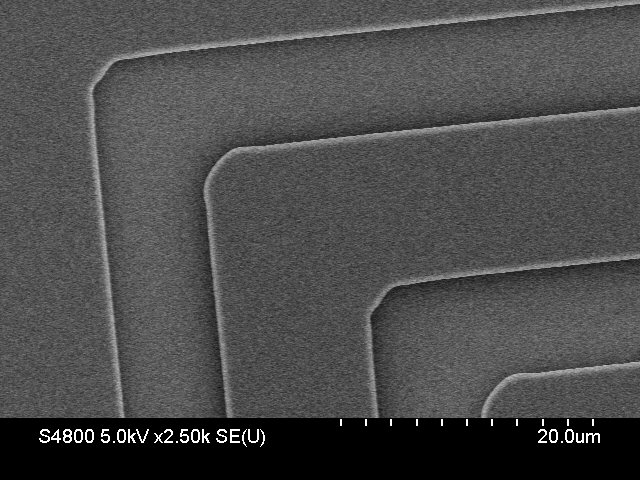
\includegraphics{data/sem/b2d33_q34.jpg}}
      	\caption{No significant differences can be seen between the inverses of the pattern.}
      	\label{fig:b2d33_q34}
    \end{subfigure}
    \caption{SEM images of single line surrounded by multiple lines on the negative tone sample with $\tau_1 = 0.5$~min. For the structure size the width of the line is taken as guideline. For structure sizes smaller than $\sim$10$\mu$m the pattern loses all detail.}
\end{figure*}

\begin{figure*}[htb]
    \centering
%     \begin{subfigure}[t]{0.24\linewidth}
%  	\centering
%  	\resizebox{\linewidth}{!}{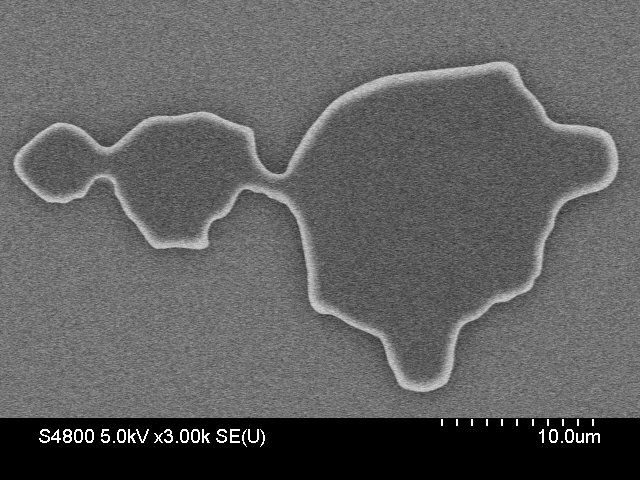
\includegraphics{data/sem/b2d33_q35.jpg}}
%  	\caption{SEM}
%  	\label{fig:b2d33_q35}
% \end{subfigure}
% \hfill
    \begin{subfigure}[t]{0.32\linewidth}
  	 	\resizebox{\linewidth}{!}{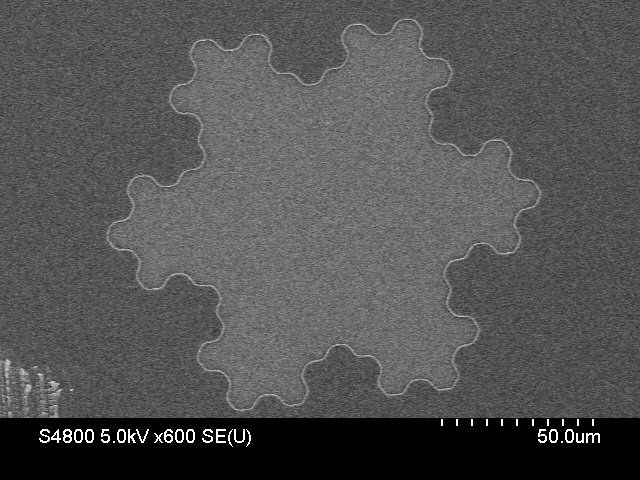
\includegraphics{data/sem/b2d36_q36.jpg}}
  	    \caption{Structure size of $\sim$20$\mu$m. There is already significant loss of detail at these structure sizes.}
  	    \label{fig:b2d36_q36}
    \end{subfigure}
    \hfill
    \begin{subfigure}[t]{0.32\linewidth}
      	\resizebox{\linewidth}{!}{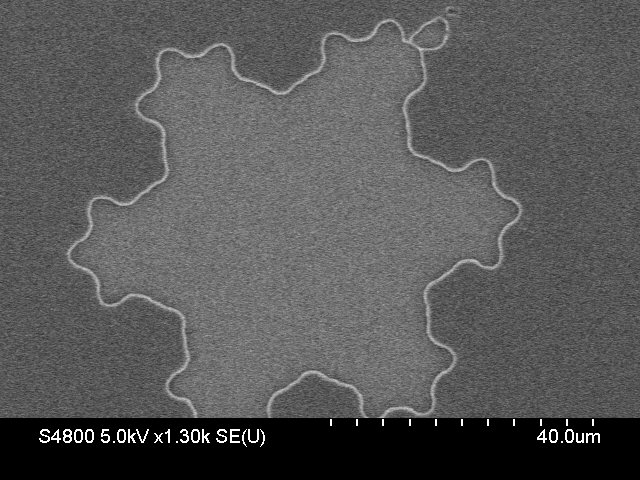
\includegraphics{data/sem/b2d36_q37.jpg}}
      	\caption{Structure size of $\sim$10$\mu$m. All fine detail is lost.}
      	\label{fig:b2d36_q37}
    \end{subfigure}
    \hfill
    \begin{subfigure}[t]{0.32\linewidth}
      	\resizebox{\linewidth}{!}{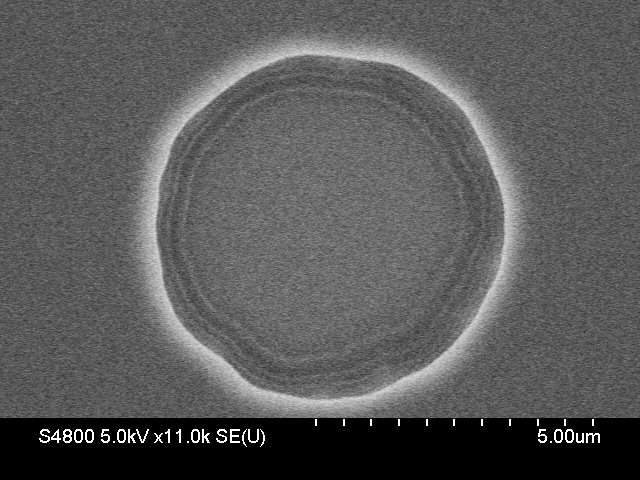
\includegraphics{data/sem/b2d38_q38.jpg}}
      	\caption{Complete loss of detail for structure size $\sim$1$\mu$m.}
      	\label{fig:b2d38_q38}
    \end{subfigure}
% \hfill
%     \begin{subfigure}[t]{0.24\linewidth}
%  	\centering
%  	\resizebox{\linewidth}{!}{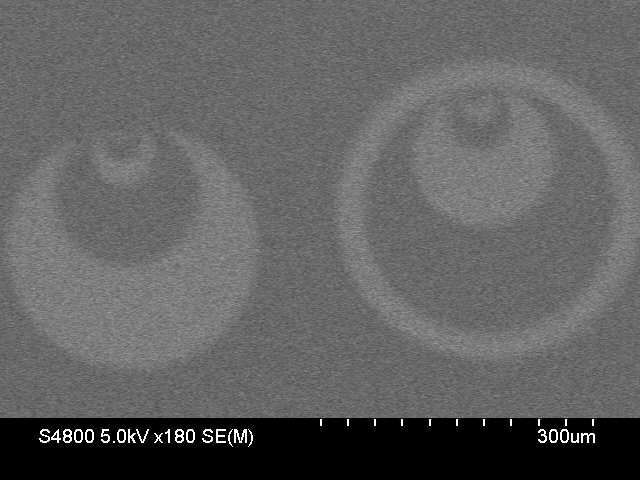
\includegraphics{data/sem/b2d39_q39.jpg}}
%  	\caption{SEM}
%  	\label{fig:b2d39_q39}
% \end{subfigure}
% \hfill
%     \begin{subfigure}[t]{0.24\linewidth}
%  	\centering
%  	\resizebox{\linewidth}{!}{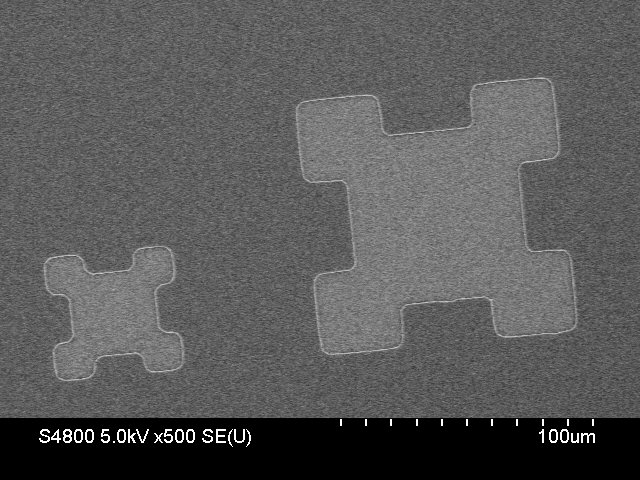
\includegraphics{data/sem/b2d40_q40.jpg}}
%  	\caption{SEM}
%  	\label{fig:b2d40_q40}
% \end{subfigure}
    \caption{SEM images of Koch snowflakes on the negative tone sample with $\tau_1=0.5$~min. For the structure size the width of one of the bulbs is taken as guideline.}
\end{figure*}

% \begin{figure*}[!t]
%     \centering
%     \begin{subfigure}[t]{0.32\linewidth}
% 	\resizebox{\linewidth}{!}{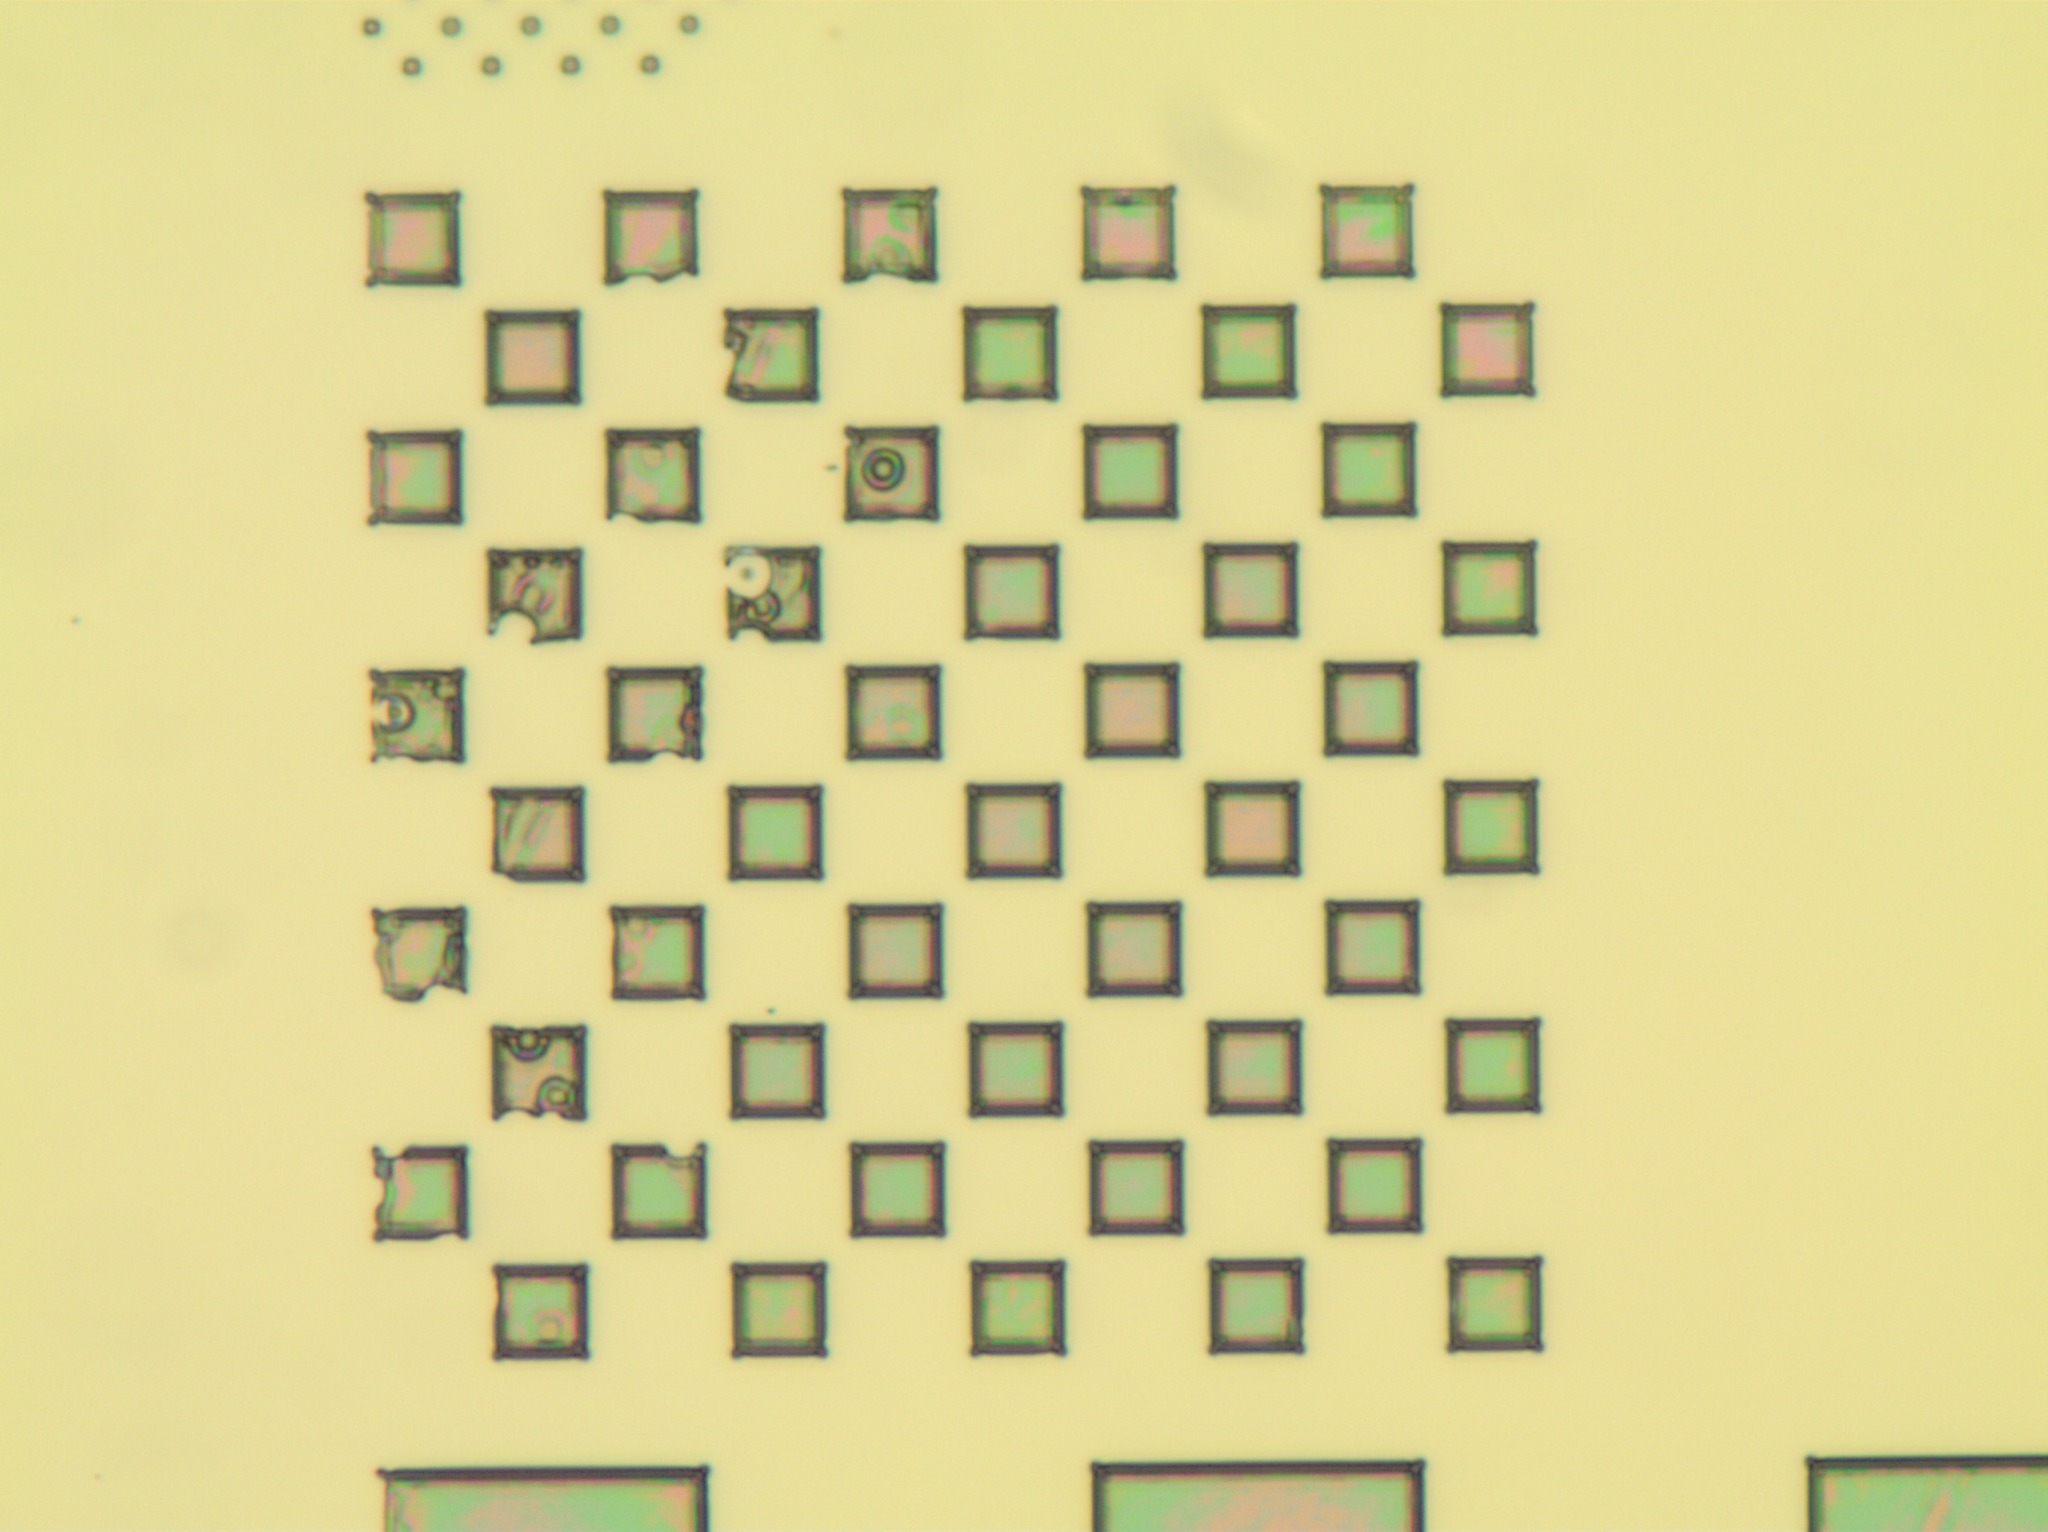
\includegraphics{data/b2i1.jpg}}
%  	\caption{Exposure time of 0.1 minutes}
%  	\label{fig:b2i1}
% \end{subfigure}
%\hfill
%     \begin{subfigure}[t]{0.32\linewidth}
% 	\resizebox{\linewidth}{!}{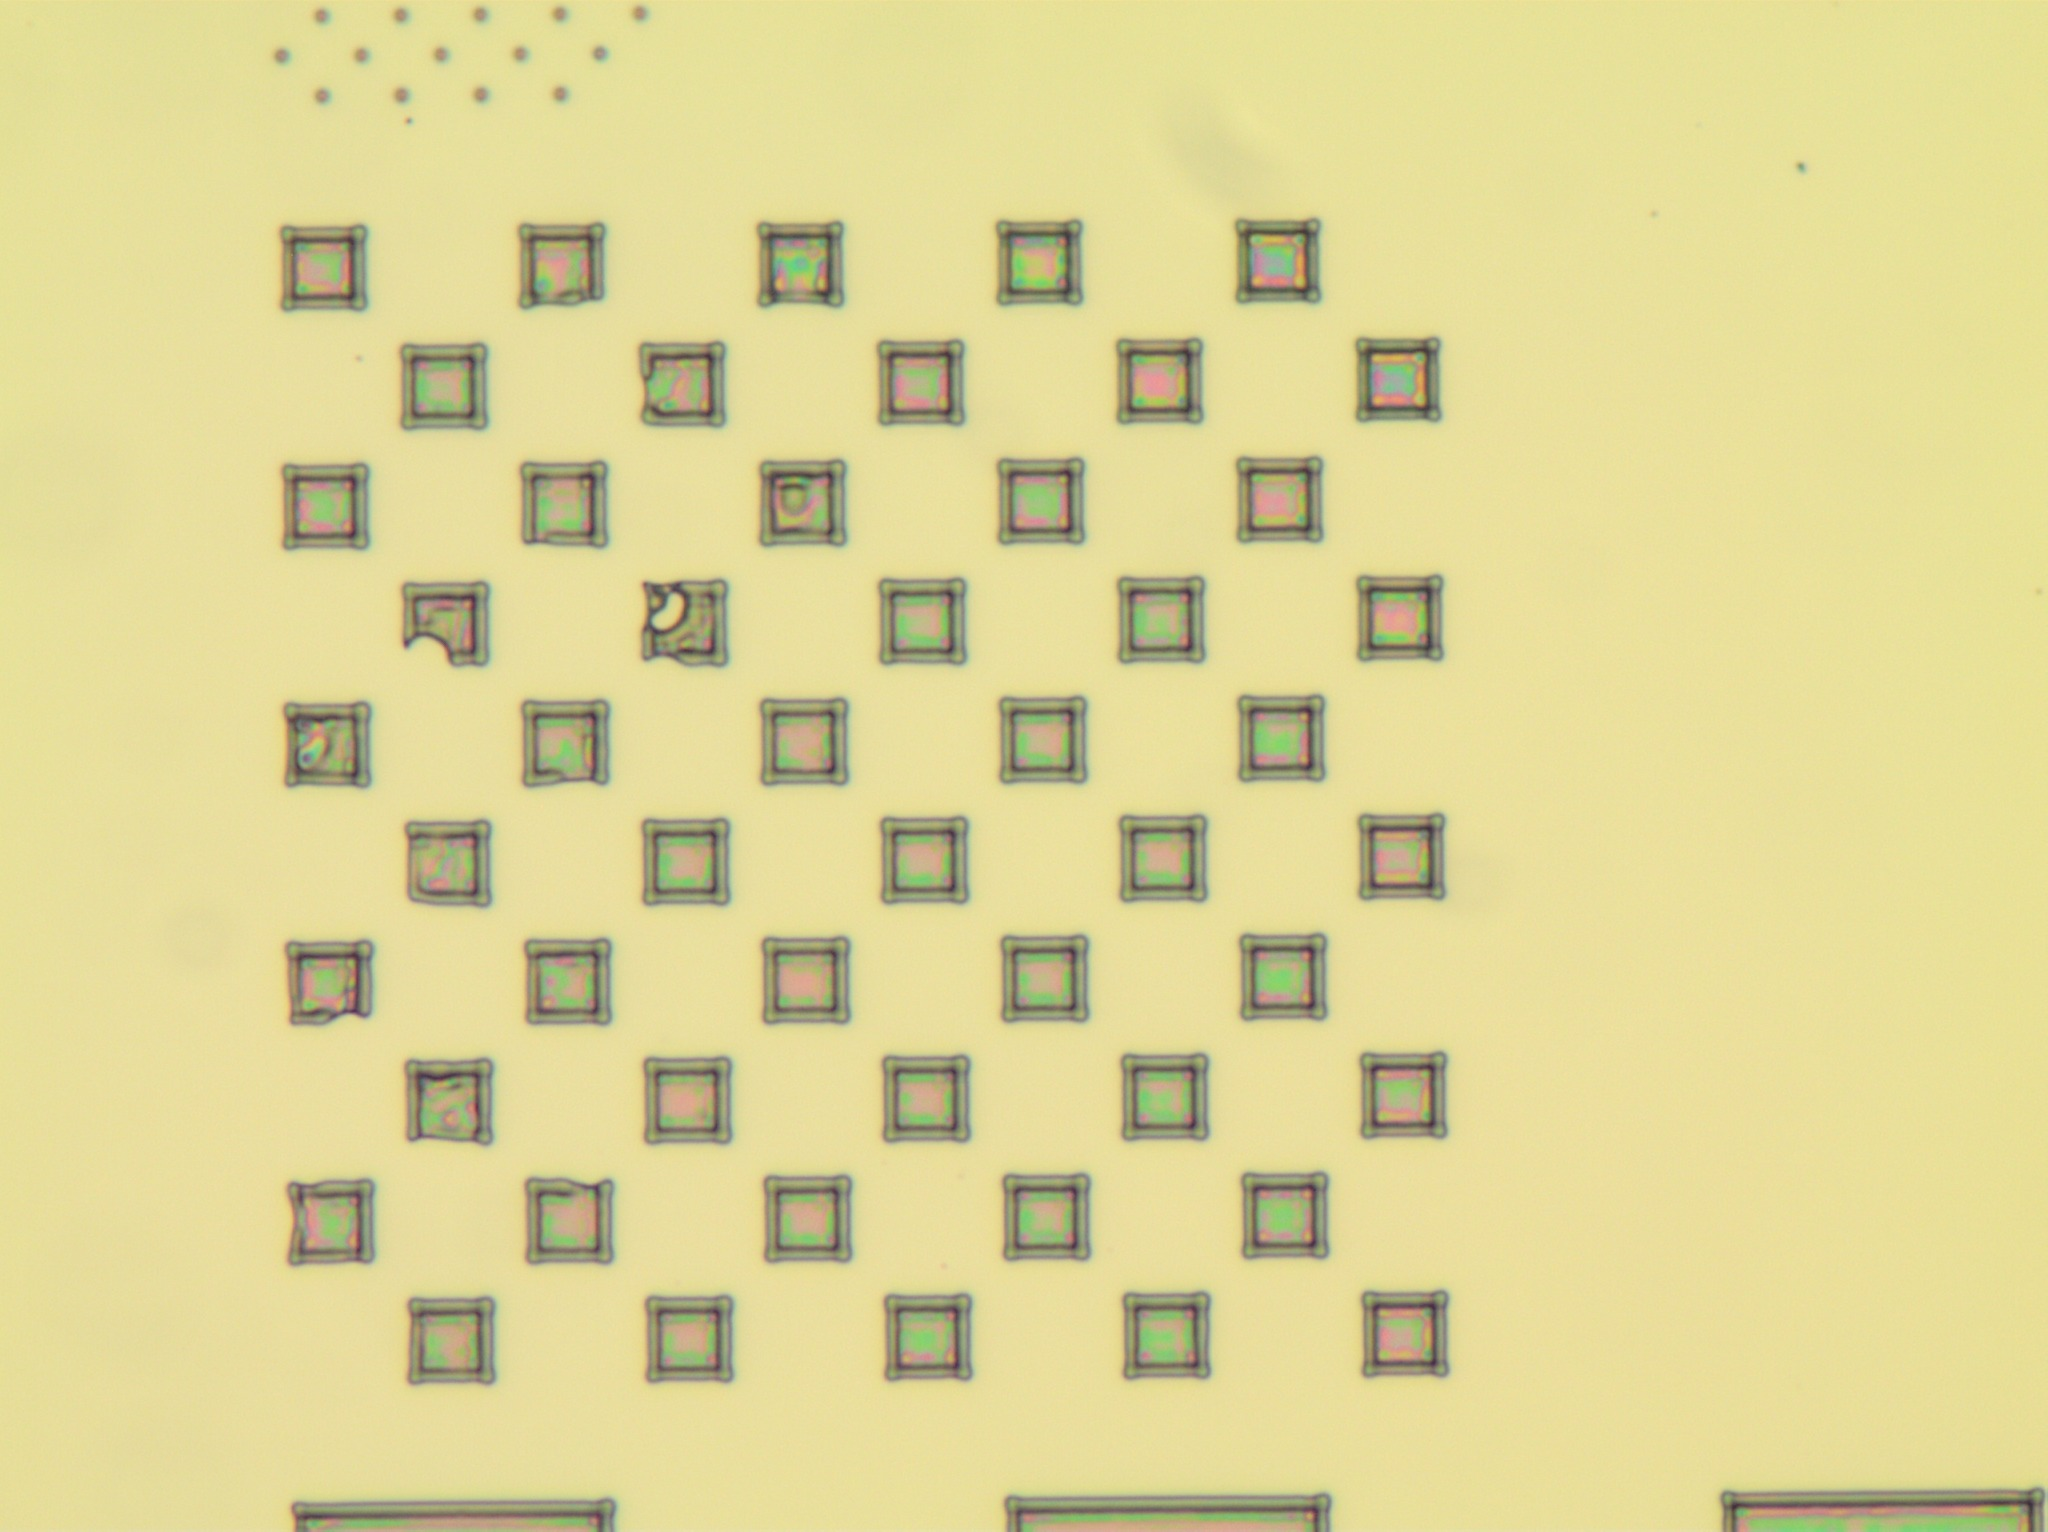
\includegraphics{data/b2h1.jpg}}
%  	\caption{Exposure time of 0.2 minutes}
%  	\label{fig:b2h1}
% \end{subfigure}
%\hfill
%     \begin{subfigure}[t]{0.32\linewidth}
% 	\resizebox{\linewidth}{!}{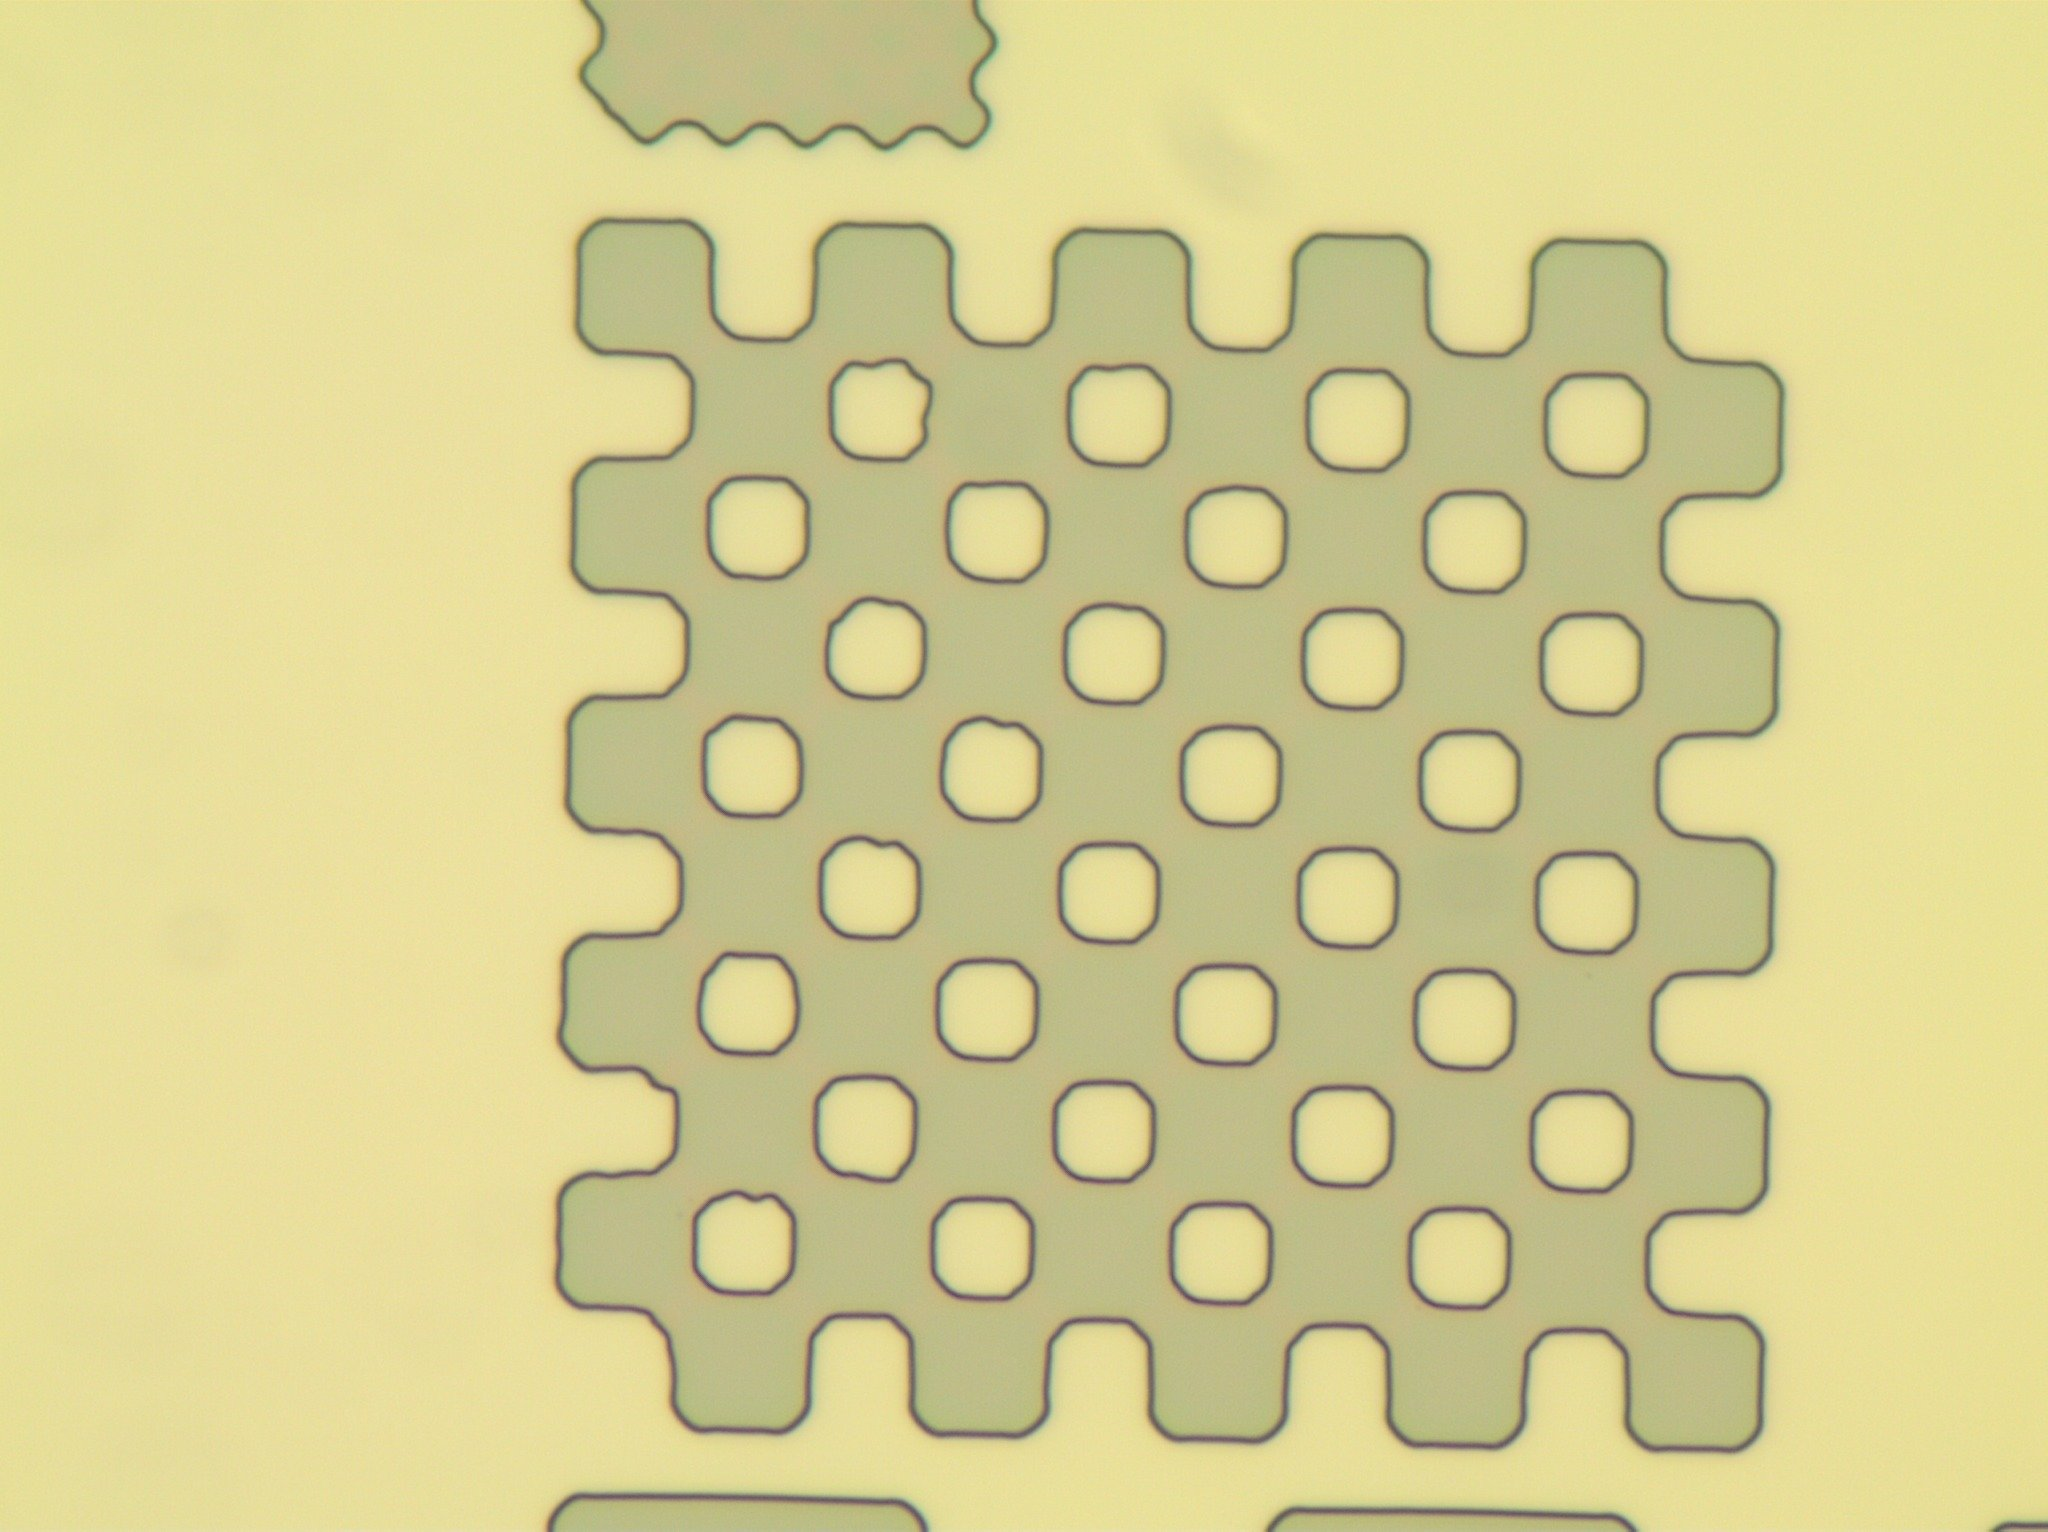
\includegraphics{data/b2d1.jpg}}
%  	\caption{Exposure time of 0.5 minutes}
%  	\label{fig:b2d1}
% \end{subfigure}
%\caption{Microscope images of the negative tone samples for several exposure times.}
%\end{figure*}


%
%  \begin{figure*}[!t]
%  	\centering
%  	\resizebox{0.33.\linewidth}{!}{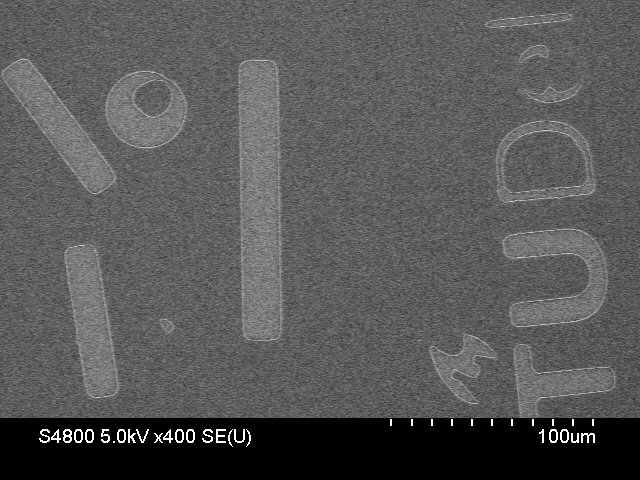
\includegraphics{data/sem/b2d41_q41.jpg}}
%  	\caption{test}
%  	\label{fig:b2d41_q41}
%  \end{figure*}
 %
 %\begin{figure*}[!t]
 %    \centering
 %    \begin{subfigure}[t]{0.24\linewidth}
 %	\resizebox{\linewidth}{!}{\includegraphics{data/sem/b3a1_q01.jpg}}
 %	\caption{SEM}
 %	\label{fig:b2d1_q1}
 %\end{subfigure}
 %\hfill
 %    \begin{subfigure}[t]{0.24\linewidth}
 %	\centering
 %	\resizebox{\linewidth}{!}{\includegraphics{data/sem/b3a2_q02.jpg}}
 %	\caption{SEM}
 %	\label{fig:b2d2_q2}
 %\end{subfigure}
 %\hfill
 %    \begin{subfigure}[t]{0.24\linewidth}
 %	\centering
 %	\resizebox{\linewidth}{!}{\includegraphics{data/sem/b3a3_q03.jpg}}
 %	\caption{SEM}
 %	\label{fig:b2d3_q3}
 %\end{subfigure}
 %    \begin{subfigure}[t]{0.24\linewidth}
 %	\centering
 %	\resizebox{\linewidth}{!}{\includegraphics{data/sem/b3a10_q10.jpg}}
 %	\caption{SEM}
 %	\label{fig:b2d10_q10}
 %\end{subfigure}
 %\end{figure*}

% \begin{figure*}[!t]
% \centering
%     \begin{subfigure}[t]{0.32\linewidth}
% 	\centering
% 	\resizebox{\linewidth}{!}{\includegraphics{data/sem/b3a4_q04.jpg}}
% 	\caption{Structure size of $\sim$32 $\mu$m.}
% 	\label{fig:b2d4_q4}
% \end{subfigure}
% \hfill
%     \begin{subfigure}[t]{0.32\linewidth}
% 	\centering
% 	\resizebox{\linewidth}{!}{\includegraphics{data/sem/b3a6_q06.jpg}}
% 	\caption{Structure size of $\sim$10 $\mu$m.}
% 	\label{fig:b2d6_q6}
% \end{subfigure}
% \hfill
%     \begin{subfigure}[t]{0.32\linewidth}
% 	\centering
% 	\resizebox{\linewidth}{!}{\includegraphics{data/sem/b3a8_q08.jpg}}
% 	\caption{Structure size of $\sim$3 $\mu$m.}
% 	\label{fig:b2d8_q8}
% \end{subfigure}
% \end{figure*}
